%% Writing a thesis in LaTeX - http://tug.org/pracjourn/2008-1/mori/mori.pdf
%\RequirePackage[l2tabu, orthodox]{nag} % tells you of any bad LaTeX usage
                                       % must be first thing in class (with the exception of comments)
%% There is one option you should define; oneside or twoside
%% Use twoside for your viva docs (examiners hate long docs they need to carry around)
%% and oneside for the final thing you submit to the library.  Note that margins will
%% change accordingly

\documentclass[twoside]{umCris}  % custom University of Malta project/dissertation/thesis
\newcommand{\e}[1]{\ensuremath{\times10^{#1}}}
\newcommand{\mnn}{\ensuremath{^{-1}}}
\newcommand{\R}{{\large\texttt{R}}}
\newcommand{\trm}{\texttt{transmem}}
\newcommand{\includeArticle}[1]{
  \clearpage
    {\floatstyle{boxed}
    \restylefloat{figure}
    \begin{figure}\centering
        \includegraphics[width=0.95\textwidth, page = {#1}, trim={1.2cm 1.3cm 1.2cm 1cm}, clip]{App/images/Desalination2020}
    \end{figure}}}
\newcommand{\includeManual}[1]{
  \clearpage
    {\floatstyle{boxed}
    \restylefloat{figure}
    \begin{figure}\centering
        \includegraphics[width=0.95\textwidth, page = {#1}, trim={1.6cm 1cm 1.6cm 1.5cm}, clip]{App/images/transmem_0.1.0.pdf}
    \end{figure}}}


%\usepackage[sort&compress]{natbib} % SORT Y CONPRESS FEATURE (?)

%% **************** (Your) Packages (Start) ******************
%\usepackage[spanish]{babel}\decimalpoint
%\usepackage[utf8]{inputenc} % Non ASCII characters
\usepackage{graphicx, float, xcolor}
\usepackage[version=4]{mhchem}
\usepackage[font=small, skip=3pt]{caption}
\usepackage{multirow}
\usepackage{dcolumn} \newcolumntype{d}[1]{D{.}{.}{#1}} %align numbers by decimal dot
\usepackage{textcomp}%\textregistered\textcopyright
\usepackage[switch, modulo]{lineno}
\usepackage{wrapfig}
\usepackage[percent]{overpic}
\usepackage{tikz}
\usetikzlibrary{shapes}
\usepackage{chemfig}
    \setchemfig{
        angle increment=15,
        atom sep=\bndlen,
        bond offset=1pt,
        double bond sep=3pt,
        cram width=\cramwid,
        compound sep=5.0em,
        scheme debug=false,
        bond join=true,
        chemfig style={line width=\lnwid},
        arrow style={line width=\lnwid},
    }

\newcommand{\bndlen}{2.0em}
\newcommand{\bndlenshort}{0.5}
\newcommand{\bndlenshorter}{0.75}
\newcommand{\bndlenlonger}{1.5}
\newcommand{\bndlenlong}{1.8}
\newcommand{\lnwid}{0.7pt}
\newcommand{\cramwid}{0.3em}
%\usepackage[dvipsnames]{xcolor} %\colorbox{lightgray}{word}

%Tablas chuscas: https://inf.ethz.ch/personal/markusp/teaching/guides/guide-tables.pdf
\renewcommand{\arraystretch}{1.2}
%\begin{tabular}{@{}lll@{}} 
%Párrafos lindos sin indentar:
\parskip = 8pt plus 6pt minus 4pt
\setlength{\parindent}{0em}
% \listfiles % uncomment this to know which packages you are using
              % the list of packages will be in the bottom of the .log file

%% Note that packges may already be loaded from the um (and memoir) classes.
%% Do not add your packages to the template, but rather add them here.

%% ***************** (Your) Packages (End) *******************


%% **************** (Your) Data (Start) ******************

\title{Membrana Polimérica de Inclusión\\Para Recobro y Concentración de Litio\\A partir de Agua de Mar}  % use \\ here otherwise you get a justified title
                                                    % note capitalization of the title (only common 
                                                    % words in lower case)
\tagline{Tesis de Maestría}                     % tag line
\author{Q. Cristhian Paredes Cardona}                           % your name
\authorID{51949049-9}                           % your University Identifier
\supervisor{\\\textbf{Dr. Eduardo Rodríguez de San Miguel Guerrero}}                             % your supervisor(s) name - no . in Dr
%\cosupervisor{Dr Who}                               % your cosupervisor(s) name - no . in Dr ** OPTIONAL ** 
                                                    % simply comment out the above line if absent
% JURADO
\president{Dr. Joaquín Palacios Alquisira}
\vocala{Dr.  Luis Felipe del Castillo Dávila}
\vocalb{Dra. María del Pilar Cañizares Macias}
\vocalc{Dra. Flora Emperatriz Mercader Trejo}
\secretary{Dr. Julio César Aguilar Cordero}  
\department{Programa de Maestría y Doctorado en Ciencias Químicas\\[1ex]Departamento de Química Analítica}      % your department (e.g. Artifical Intelligence)
\faculty{Facultad de Química}                      % your faculty (e.g. ICT)
\workplace{Laboratorio 109, Departamento de Química Analítica, División de Estudios de Posgrado, Edificio B, Facultad de Química, Ciudad Universitaria, UNAM.\\Ciudad de México, México}
\degree{Maestro en Ciencias}                      % the degree you are reading
                                                    % note the \ after the dot, so not to consider it a fullstop
\doctype{Tesis}                              % the type of document (fyp, dissertation, thesis)
\degreedate{Mayo, 2020}                        % when did you submit -- officially after your corrections !
%%\subjectcode{ICS5200}                               % the study unit-code (currently not used)

%% ***************** (Your) Data (End) *******************


%% ******** (Your) Document Settings (Start) *************

% You should have an images directory in every chapX subdir
% NOTE:  Trailing / for subdirs is required.
\graphicspath{{./images/}{./chap1/images/}}   % Paths where to look for images, if defined "images" must always be there as it holds the images in-use by the template.

\makeindex

%% ********* (Your) Document Settings (End) **************

% DOCTOR'S (JP) ORDERS: MAKE SURE TO READ MY TWO BLOG ENTRIES WITH
% CONTENT AND LaTeX TIPS FOR YOUR WRITE-UP.  THESE ARE BASED ON  
% EXAMINER'S FEEDBACK
%
% URLS:
% https://bitsilla.com/blog/2019/03/content-tips-for-your-dissertation-or-project-write-up/
% https://bitsilla.com/blog/2019/01/latex-tips-for-your-dissertation-or-project-write-up/

% end the preamble and start the document
\usepackage{hyphenat}
 \hyphenation{mate-máti-cas recu-perar enca-re-ci-mien-to vehí-culos manu-fac-tura volu-men pre-sen-cia pre-fe-ren-cial disuel-tos herra-mien-tas varian-za gene-ra-ción desa-rro-lla-dores varian-za con-si-de-rado proba-ble-mente ener-gé-tico volu-men ante-rior-es  acti-vi-da-des infle-xion di-lui-do estos sepa-ra-ción mine-ra-les varia-ble míni-mos desio-ni-za-da}
 


\begin{document}
% Include before \begin{document}:
% \usepackage{tikz}
% \usetikzlibrary{shapes}
% Load % Include before \begin{document}:
% \usepackage{tikz}
% \usetikzlibrary{shapes}
% Load % Include before \begin{document}:
% \usepackage{tikz}
% \usetikzlibrary{shapes}
% Load \input{shapesforcaptions.tex} after \begin{document}
\newcommand{\circleblck}{\raisebox{0.5pt}{\tikz{\node[draw,scale=0.4,circle,fill=black](){};}}}
\newcommand{\circlewht}{\raisebox{0.5pt}{\tikz{\node[draw,scale=0.4,circle,fill=none](){};}}}

\newcommand{\squareblck}{\raisebox{0.5pt}{\tikz{\node[draw,scale=0.4,regular polygon, regular polygon sides=4,fill=black](){};}}}
\newcommand{\squarewht}{\raisebox{0.5pt}{\tikz{\node[draw,scale=0.4,regular polygon, regular polygon sides=4,fill=none](){};}}}
\newcommand{\squarerttdblck}{\raisebox{0.5pt}{\tikz{\node[draw,scale=0.4,regular polygon, regular polygon sides=4,fill=black,rotate=45](){};}}}
\newcommand{\squarerttdwht}{\raisebox{0.5pt}{\tikz{\node[draw,scale=0.4,regular polygon, regular polygon sides=4,fill=none,rotate=45](){};}}}

\newcommand{\triangleupblck}{\raisebox{0.5pt}{\tikz{\node[draw,scale=0.3,regular polygon, regular polygon sides=3,fill=black](){};}}}
\newcommand{\triangleupwht}{\raisebox{0.5pt}{\tikz{\node[draw,scale=0.3,regular polygon, regular polygon sides=3,fill=none](){};}}}
\newcommand{\triangledownblck}{\raisebox{0.5pt}{\tikz{\node[draw,scale=0.3,regular polygon, regular polygon sides=3,fill=black,rotate=180](){};}}}
\newcommand{\triangledownwht}{\raisebox{0.5pt}{\tikz{\node[draw,scale=0.3,regular polygon, regular polygon sides=3,fill=none,rotate=180](){};}}}
\newcommand{\trianglerigthblck}{\raisebox{0.5pt}{\tikz{\node[draw,scale=0.3,regular polygon, regular polygon sides=3,fill=black,rotate=270](){};}}}

\newcommand{\starfvpointsblck}{\raisebox{0.0pt}{\tikz{\node[draw, scale = 0.85, star, star points=5, star point ratio=.35, fill=black, rotate = 180](){};}}}
\newcommand{\starfvpointswht}{\raisebox{0.0pt}{\tikz{\node[draw, scale = 0.85, star, star points=5, star point ratio=.35, fill=white, color = white, rotate = 180](){};}}}

% Inside \caption{} use \protect:
%\caption{This is an inverted green triangle in a figure caption (\protect\triangleupblck).}


% Fuego acustico after \begin{document}
\newcommand{\circleblck}{\raisebox{0.5pt}{\tikz{\node[draw,scale=0.4,circle,fill=black](){};}}}
\newcommand{\circlewht}{\raisebox{0.5pt}{\tikz{\node[draw,scale=0.4,circle,fill=none](){};}}}

\newcommand{\squareblck}{\raisebox{0.5pt}{\tikz{\node[draw,scale=0.4,regular polygon, regular polygon sides=4,fill=black](){};}}}
\newcommand{\squarewht}{\raisebox{0.5pt}{\tikz{\node[draw,scale=0.4,regular polygon, regular polygon sides=4,fill=none](){};}}}
\newcommand{\squarerttdblck}{\raisebox{0.5pt}{\tikz{\node[draw,scale=0.4,regular polygon, regular polygon sides=4,fill=black,rotate=45](){};}}}
\newcommand{\squarerttdwht}{\raisebox{0.5pt}{\tikz{\node[draw,scale=0.4,regular polygon, regular polygon sides=4,fill=none,rotate=45](){};}}}

\newcommand{\triangleupblck}{\raisebox{0.5pt}{\tikz{\node[draw,scale=0.3,regular polygon, regular polygon sides=3,fill=black](){};}}}
\newcommand{\triangleupwht}{\raisebox{0.5pt}{\tikz{\node[draw,scale=0.3,regular polygon, regular polygon sides=3,fill=none](){};}}}
\newcommand{\triangledownblck}{\raisebox{0.5pt}{\tikz{\node[draw,scale=0.3,regular polygon, regular polygon sides=3,fill=black,rotate=180](){};}}}
\newcommand{\triangledownwht}{\raisebox{0.5pt}{\tikz{\node[draw,scale=0.3,regular polygon, regular polygon sides=3,fill=none,rotate=180](){};}}}
\newcommand{\trianglerigthblck}{\raisebox{0.5pt}{\tikz{\node[draw,scale=0.3,regular polygon, regular polygon sides=3,fill=black,rotate=270](){};}}}

\newcommand{\starfvpointsblck}{\raisebox{0.0pt}{\tikz{\node[draw, scale = 0.85, star, star points=5, star point ratio=.35, fill=black, rotate = 180](){};}}}
\newcommand{\starfvpointswht}{\raisebox{0.0pt}{\tikz{\node[draw, scale = 0.85, star, star points=5, star point ratio=.35, fill=white, color = white, rotate = 180](){};}}}

% Inside \caption{} use \protect:
%\caption{This is an inverted green triangle in a figure caption (\protect\triangleupblck).}


% Fuego acustico after \begin{document}
\newcommand{\circleblck}{\raisebox{0.5pt}{\tikz{\node[draw,scale=0.4,circle,fill=black](){};}}}
\newcommand{\circlewht}{\raisebox{0.5pt}{\tikz{\node[draw,scale=0.4,circle,fill=none](){};}}}

\newcommand{\squareblck}{\raisebox{0.5pt}{\tikz{\node[draw,scale=0.4,regular polygon, regular polygon sides=4,fill=black](){};}}}
\newcommand{\squarewht}{\raisebox{0.5pt}{\tikz{\node[draw,scale=0.4,regular polygon, regular polygon sides=4,fill=none](){};}}}
\newcommand{\squarerttdblck}{\raisebox{0.5pt}{\tikz{\node[draw,scale=0.4,regular polygon, regular polygon sides=4,fill=black,rotate=45](){};}}}
\newcommand{\squarerttdwht}{\raisebox{0.5pt}{\tikz{\node[draw,scale=0.4,regular polygon, regular polygon sides=4,fill=none,rotate=45](){};}}}

\newcommand{\triangleupblck}{\raisebox{0.5pt}{\tikz{\node[draw,scale=0.3,regular polygon, regular polygon sides=3,fill=black](){};}}}
\newcommand{\triangleupwht}{\raisebox{0.5pt}{\tikz{\node[draw,scale=0.3,regular polygon, regular polygon sides=3,fill=none](){};}}}
\newcommand{\triangledownblck}{\raisebox{0.5pt}{\tikz{\node[draw,scale=0.3,regular polygon, regular polygon sides=3,fill=black,rotate=180](){};}}}
\newcommand{\triangledownwht}{\raisebox{0.5pt}{\tikz{\node[draw,scale=0.3,regular polygon, regular polygon sides=3,fill=none,rotate=180](){};}}}
\newcommand{\trianglerigthblck}{\raisebox{0.5pt}{\tikz{\node[draw,scale=0.3,regular polygon, regular polygon sides=3,fill=black,rotate=270](){};}}}

\newcommand{\starfvpointsblck}{\raisebox{0.0pt}{\tikz{\node[draw, scale = 0.85, star, star points=5, star point ratio=.35, fill=black, rotate = 180](){};}}}
\newcommand{\starfvpointswht}{\raisebox{0.0pt}{\tikz{\node[draw, scale = 0.85, star, star points=5, star point ratio=.35, fill=white, color = white, rotate = 180](){};}}}

% Inside \caption{} use \protect:
%\caption{This is an inverted green triangle in a figure caption (\protect\triangleupblck).}


% Fuego acustico
\interfootnotelinepenalty=10000
\renewcommand{\tablename}{Tabla}
\renewcommand{\figurename}{Figura}
\renewcommand{\indexname}{Índice}
\newcommand{\ChapBib}[1]{\bibliographystyle{um-plainnat}{\footnotesize\bibliography{#1}}}
\newsubfloat{table}


\frontmatter 
    \maketitle
         %Delete hypenation: :O
        \pretolerance=10000
        \tolerance=2000 
        \emergencystretch=10pt
    \begin{copyrightenv}\end{copyrightenv}
    \begin{juries}\end{juries}
%    %\begin{originality}\end{originality}   
    \begin{dedication}
{\large{A Vickita y a Branditon,}}\\[2mm]
que son mis flechas del anhelo hacia la otra orilla...
\end{dedication}

        % include a dedication.tex file
    \begin{acknowledgements}
Agradezco a la espléndida Universidad Nacional Autónoma de México que me acogió con calidez y me hizo sentir siempre como parte de su hermosa comunidad. Agradezco a mi tutor, el Dr. Eduardo Rodríguez de San Miguel, por ser el arquitecto del proyecto de investigación y por compartirme conocimientos que atesoraré toda la vida. Agradezco a los respetados miembros de mi Jurado Evaluador por sus oportunas observaciones y correcciones que fueron fundamentales para mejorar la calidad de este manuscrito. También agradezco al Consejo Nacional de Ciencia y Tecnología, por administrar y compartirme parte de los recursos de los contribuyentes del hermoso pueblo Mexicano, quienes de manera generosa y desinteresada financiaron mi estancia es su lindo país lleno de arte, historia, magia y color, bajo el número de CVU 918468. Llevaré siempre a México y a su ciudadanía incrustados en mi corazón. 

Del personal académico de la UNAM agradezco a la Dra. Josefina de Gyves por los consejos y el apoyo que me otorgó durante la maestría. Aprecio los servicios técnicos de QFB. Guadalupe Espejel y Qca. Nadia Munguía. Valoro la compañía y el interés de mis atentos amigos compañeros de laboratorio, y la de mi amigo Corzo, quien tuvo la fabulosa idea de considerar a la UNAM como casa de estudios para adelantar mis estudios de posgrado.

Agradezco a mi amada Alma Mater, la Universidad Nacional de Colombia, y a las buenas personas que me crucé en mi paso por esa Institución. En especial agradezco a los Profesores Jesús Agreda y Eliana Castillo, por creer en mí y por su influencia enorme en mi forma de ver el mundo que me rodea.

Debo agradecer a mis padres Albita Cardona y Víctor Paredes, quienes con su ejemplo, su apoyo y su amor, me han motivado para seguir trabajando en ser cada vez una mejor persona. También les debo a ellos la recolección de las muestras de agua de mar que fueron usadas en la etapa final de este trabajo. A mis hermanos Vickita y Branditon, que siempre estuvieron presentes en mis felicidades y mis penurias. Me considero muy afortunado de tenerlos en mi vida. 

Finalmente quiero hacer una mención muy especial a Alexandra Elbakyan por su incansable esfuerzo en remover las barreras del acceso al conocimiento. %, y finalmente, al Maestro de Capilla Juan Sebastian Bach, por su obra sublime que siempre me logró reconfortar en los momentos difíciles y que, a mi modo de ver, siempre será el regalo más hermoso que pudo alguien haber hecho a la humanidad.
\end{acknowledgements}   % include an acknowledgements.tex file
    %% For tips on how to write a great abstract, have a look at
%%	-	https://www.cdc.gov/stdconference/2018/How-to-Write-an-Abstract_v4.pdf (presentation, start here)
%%	-	https://users.ece.cmu.edu/~koopman/essays/abstract.html
%%	-	https://search.proquest.com/docview/1417403858
%%  - 	https://www.sciencedirect.com/science/article/pii/S037837821830402X

\begin{resumen}%\addcontentsline{toc}{chapter}{Resumen}
\selectlanguage{spanish}
Este trabajo de tesis presenta una metodología para extraer ion litio que se encuentra a baja concentración en medios acuosos, usando una membrana polimérica de inclusión que incorpora los extractactes comerciales LIX-54-100 y Cyanex~923, en un soporte polimérico de triacetato de celulosa. Se logró la extracción de ion litio empleando, como matriz de extracción, disoluciones ideales, mezclas sintéticas donde el ion litio está presente en conjunto con otros cationes, una matriz de agua de mar sintética simplificada, y muestras de agua de mar natural. El sistema presenta buena selectividad por el el ion litio frente los cationes potasio y sodio. Es posible concentrar el ion litio usando la metodología propuesta, y la membrana es medianamente estable durante los primeros diez ciclos de transporte. La optimización del sistema se hizo por medio de diseños experimentales factoriales fraccionados de dos niveles y siguiendo el algoritmo de optimización simplex de paso variable.

Los perfiles de transporte fueron ajustados a una nueva ecuación empírica que se propone en este trabajo. El modelo presenta un excelente ajuste con los datos experimentales, y sus parámetros ajustables se pueden relacionar con la velocidad y con la eficiencia del proceso de transporte. Esto permitió que dichos parámetros pudieran ser usados exitosamente como variables respuesta en los diseños experimentales desarrollados.

En el desarrollo del proyecto se escribió un paquete para el programa de computación científica y representaciones gráficas \R. El propósito del paquete \verb|transmem| es facilitar el tratamiento sistemático y reproducible de los datos generados en experimentos de transporte a través de membranas, con el fin de obtener parámetros de desempeño del sistema y de producir representaciones gráficas de alta calidad. El paquete está disponible en el repositorio oficial de \R, y actualmente se encuentra en proceso de adaptación a una interfaz gráfica interactiva (tipo aplicación web), que permite el aprovechamiento de sus funcionalidades por parte de usuarios que no se encuentran familiarizados con el lenguaje de programación \R.
%Los resultados más relevantes del presente trabajo fueron recopilados en un artículo aceptado para su publicación en la revista \textit{Desalination}.\footnote{ISSN: 0011-9164}

\end{resumen}
%\begin{abstract}\addcontentsline{toc}{chapter}{Abstract}
%\textbf{This is the abstract.}
%\end{abstract}\if@openright\cleardoublepage\else\clearpage\fi
    \tableofcontents*\if@openright\cleardoublepage\else\clearpage\fi
    \listoffigures*\if@openright\cleardoublepage\else\clearpage\fi
    \listoftables*\if@openright\cleardoublepage\else\clearpage\fi
    %% will only print what is used ... useful.
%% also acronyms are clickable, which is awesome

\chapter*{Lista de Abreviaturas}\addcontentsline{toc}{chapter}{Lista de abreviaturas}
\markboth{Lista de Abreviaturas}{Lista de Abreviaturas}
\enlargethispage{2\baselineskip}               
\vspace{-1.5cm}\begin{acronym}\itemsep-2.5pt\parsep-2.5pt %% if you remove these spacing params this list becomes huge!
\acro{BLM}{Membrana Liquida de Bulto}
\acro{CTA}{Triacetato de celulosa}% (\textit{Cellulose triacetate})}
\acro{CRAN}{\textit{Comprehensive R Archive Network}}
\acro{DCM}{Diclorometano}
\acro{EV}{Vehículo Eléctrico}% (\textit{Electric Vehicles})}
\acrodefplural{EV}[EVs]{Vehículos Eléctricos}
\acro{FAAS}{Espectrometría de Absorción Atómica por Llama}
\acro{FAES}{Espectrometría de Emisión Atómica por Llama}
\acro{FPS}{Fotogramas por Segundo}
\acro{GIU}{Interfaz Gráfica de Usuario}
\acro{LCE}{Carbonato de Litio Equivalente}% (\textit{Lithium Carbonate Equivalent})}
\acro{LIB}{Batería de Ion de Litio}% (\textit{Lithium Ion Battery)}}
\acrodefplural{LIB}[LIBs]{Baterías de Ion de Litio}
\acro{NIPALS}{Mínimos Cuadrados Parciales Iterativos No Lineales}
\acro{NLS}{Regresión no lineal por mínimos cuadrados}
\acro{NPOE}{1-(2-nitrofenoxi)octano}
\acro{PCA}{Análisis de Componentes Principales}
\acro{PET}{Poli(tereftalato de etileno)}% (\textit{Poly(ethylene Terephthalate)})}
\acro{PIM}{Membrana Polimérica de Inclusión}% (\textit{Polymer Inclusion Membrane})}
\acrodefplural{PIM}[PIMs]{Membranas Poliméricas de Inclusión}
\acro{PVC}{Poli(cloruro de vinilo)}
\acro{PWM}{Modulador de Ancho de Pulso}% (\textit{Pulse Width Modulator})}
\acro{RGB}{Rojo-Verde-Azul}% (\textit{Red-Green-Blue})}
\acro{RPM}{Revoluciones por Minuto}
\acro{SLM}{Membrana Liquida Soportada}
\acrodefplural{SLM}[SLMs]{Membranas Liquidas Soportadas}
\acro{SSX}{Extracción Sinérgica con Disolventes}
\acrodefplural{SSX}{Extracciones Sinérgicas con Disolventes}
\acro{TBEP}{Tris(2-butoxietil)fosfato}
\acro{TEHP}{Tris(2-etilhexil)fosfato}
\acro{USD}{Dólares Estadounidenses}% (\textit{United States Dollar)}}
\end{acronym}
%LCE is the industry standard terminology for, and is equivalent to, Li2CO3. 1 ppm Li metal is equivalent to 5.323


\chapter*{Lista de Compuestos Orgánicos}%Estructuras de extractantes, plastificantes y demás
\addcontentsline{toc}{chapter}{Lista de compuestos orgánicos}
% https://www.researchgate.net/publication/325102342_A_Review_on_the_Separation_of_Lithium_Ion_from_Leach_Liquors_of_Primary_and_Secondary_Resources_by_Solvent_Extraction_with_Commercial_Extractants

{\footnotesize
\begin{tabular}{p{4cm}p{3.4cm}p{3.4cm}p{3.3cm}}
    \textbf{CTA}\newline Triacetato de celulosa \newline\vspace{6ex}
    {\chemfig{-[@{upleft, .5}:20,1]O-[:-20, 1.1]<[:35, 1.07](-[:-120,0.8]-[:-30,.8]OR)-[:-15,,,,line width=2.4pt]O>[:60, 1.1](-[@{upright,0.7}:-20,1]O-[:20])-[:-160,.95](-[:70,.8]OR)-[:165,.8](-[:-155,.7]RO)-[:-123,1.35]}}
    \polymerdelim[delimiters ={[]}, height = 35pt, depth = 20pt, indice = n]{upleft}{upright}\vspace{0.7ex}
    \newline donde R es acetato.
     &
    \textbf{LIX-54-100}\newline Mezcla de $\beta$-dicetonas \vspace{2ex}\newline
      \chemfig{O=[:180]
        (-[:120](-[:60](=[:0]O)(-[:120,,,1]R_1)))
        ((-[:-120,,,]R_2))}\newline\vspace{0.7ex}\newline donde R$_1$ y R$_2$ son grupos fenil o heptil
    &
    \textbf{D2EHPA}\newline Ácido di-2-etilhexil\newline fosfórico \vspace{2ex}\newline
        \chemfig{P(=[:90]O)(-[:-45,1.3]OH)(-[:-75,1.2]O-[:-35,1,,1]C_8H_{17})(-[:-120,1.32]O-[:-75,1,,1]C_8H_{17})}\newline
    &
    \textbf{Cyanex 923}\newline Mezcla de óxidos de\newline trialquilfosfinas\vspace{2ex}\newline
    \chemfig{P(=[:90]O)(-[:-45,1.3]R_3)(-[:-75,1.3]R_2)(-[:-120,1.3]R_1)}\newline  \vspace{0.7ex} \newline donde R$_1$, R$_2$, y R$_3$ son cadenas alquílicas de entre 6 y 8 átomos de carbono\newline
    \\
    \textbf{TEHP}\newline Tris(2-etilhexil)fosfato  \vspace{2ex}\newline
\chemfig{P(=[:90]O)(-[:-45,1.3]O-[:-5,0.9,,1]C_8H_{17})(-[:-75,1.1]O-[:-35,1,,1]C_8H_{17})(-[:-120,1.32]O-[:-65,1,,1]C_8H_{17})}\newline
%\chemfig{P(=[:90]O)(-[:-45,1]C_8H_{17})(-[:-75,1.25]C_8H_{17})(-[:-120,1.32]H_{17}C_8)}
    &
    \textbf{TBP}\newline Tri-n-butil fosfato \vspace{2ex}\newline
\chemfig{P(=[:90]O)(-[:-45,1.3]O-[:-5,0.9,,1]C_4H_{9})(-[:-75,1.1]O-[:-35,1,,1]C_4H_{9})(-[:-120,1.32]O-[:-65,1,,1]C_4H_{9})}\newline
%\chemfig{P(=[:90]O)(-[:-45,1]C_4H_9)(-[:-75,1.25]C_4H_9)(-[:-120,1.32]H_9C_4)}
    &
    \textbf{NPOE}\newline 1-(2-nitrofenoxi)octano  \vspace{2ex}\newline
    \chemfig{O=[:-45]N^{+}(-[:45]O^{-})(-[:-90]([:-90]**6(-----(-[:30]O-[:-30]C_8H_{17})-)))}
    &
    \textbf{TBEP}\newline Tris(2-butoxietil)fosfato  \vspace{0.2ex}\newline
        \chemfig{P(=[:90]O)(-[:-45,1.3]O-[:-20]-[:-70]-[:-15]O-[:-70,,,1]C_4H_9)(-[:-75,1.2]O-[:-40]-[:-95]-[:-40]O-[:-95,,,1]C_4H_9)(-[:-120,1.32]O-[:-55]-[:-110]-[:-55]O-[:-110,1.1,,1]C_4H_9)}\newline
\end{tabular}}

\chapter*{Nomenclatura}
\addcontentsline{toc}{chapter}{Nomenclatura}
\vspace{-1cm}
\begin{tabular}{p{1.8cm} l}
    $E$         & Eficiencia en un proceso de transporte (\%)\\
    $t$         & Tiempo (generalmente en horas)\\
    $\Phi_{ali}$& Fracción remanente en la disolución de alimentación\\
    $\Phi_{rec}$& Fracción transportada a la disolución de recuperación\\
    $P$         & Coeficiente de permeabilidad (m~s\mnn)\\
    $V$         & Volumen de disolución (m$^3$ o cm$^3$)\\
    $a$         & Área expuesta de membrana (m$^2$ o cm$^2$)\\
    $Sf_{\ce{Li+}/\ce{M^n+}}$ & Factor de separación entre litio y otro catión metálico\\
    $k$         & Número de variables de un diseño experimental\\
    $n$         & Número de niveles consideradas por variable en un diseño experimental\\
    $n$         & Dimensionalidad de un espacio experimental\\
    %$A_i$       & Primer parámetro ajustable de la ecuación de Rodríguez de San Miguel et al. (2014)\\
    %$d_i$       & Segundo parámetro ajustable de la ecuación de Rodríguez de San Miguel et al. (2014)\\
    %$y_{0,i}$   & Tercero parámetro ajustable de la ecuación de Rodríguez de San Miguel et al. (2014)\\
    $\alpha_i$  & Primer parámetro ajustable de la ecuación propuesta en el Capítulo \ref{sec:NLS}\\
    $\beta_i$   & Segundo parámetro ajustable de la ecuación propuesta en el Capítulo \ref{sec:NLS}\\
    $\kappa$    & Parámetro de excentricidad de la ecuación propuesta en el Capítulo \ref{sec:NLS}\\
    $\lambda$   & Longitud de onda (nm) \\
    $Abs_{\lambda}$ & Señal de absorbancia atómica a la longitud de onda $\lambda$\\
    $Em_{\lambda}$ & Señal de emisión atómica a la longitud de onda $\lambda$\\
    $\Theta$    & Rapidez de giro de las propelas de agitación (RPM)\\
    $\Upsilon$  & Variable respuesta en un diseño experimental\\
    X\textit{i} & Variable considerada en un diseño experimental\\
    
\end{tabular}
\if@openright\cleardoublepage\else\clearpage\fi

\pagestyle{umpage}
\mainmatter 
\linenumbers
    \chapter{Introducción}

\section{Descripción del problema}\label{sec:descrip} % why is this a non trivial problem
La civilización moderna hace uso de vastas cantidades de energía para sostener distintas actividades que considera primordiales para su desarrollo. Los homínidos empezaron a dominar el fuego hace aproximadamente dos millones de años, y esto representó un punto de inflexión importante en el camino para convertirse en lo que somos nosotros ahora \citep{Gowlett2016}. Desde entonces, la combustión ha representado la fuente energética por excelencia para impulsar diversos procesos. Los recursos fósiles son el combustible más común, pero su uso presenta varias desventajas que conciernen principalmente al impacto ambiental negativo que generan y al hecho de que su disponibilidad es limitada. Por otro lado, las fuentes energéticas renovables son más limpias desde un punto de vista ambiental y en algunos casos pueden considerarse de disponibilidad ilimitada para todos los efectos prácticos. El principal problema que reside en su aprovechamiento es que su disponibilidad no es constante en el tiempo por lo que debe almacenarse eficientemente. Una forma práctica de almacenar energía es en forma de energía eléctrica. Los dispositivos de almacenamiento de energía eléctrica tienen un papel protagónico en la revolución ambiental y energética que se experimenta en el mundo actualmente. En particular, las baterías de ion de litio (LIB) han probado ser una excelente alternativa para almacenar energía eléctrica \citep{Chen2020}, y su uso se ha venido expandiendo en los últimos años.

Algunos autores consideran que la gran ganancia del mercado por parte de las LIBs puede repercutir en escasez y desabastecimiento de litio cuando la demanda supere a la oferta, en el futuro, si no se toman medidas para evitarlo \citep{SVERDRUP2016, VIKSTROM2013, Benson2017, Chagnes2015}. Actualmente, este elemento es extraído a escala industrial a partir de minerales y salmueras ubicados en algunas regiones del mundo. Igual que los combustibles fósiles, los recursos de los que el litio puede ser extraído de una forma económicamente viable usando la tecnología disponible hoy en día, son limitados. Varias posibles fuentes naturales de litio no son explotadas actualmente, principalmente porque el litio se encuentra demasiado diluido, o porque la presencia de especies interferentes que dificultan su recobro es muy alta. El litio es considerado por muchos como un elemento crítico, es decir, un elemento que presenta riesgos en su cadena de suministro \citep{Zubi2018}. Un gran número de grupos de investigación en todo el mundo trabaja muy activamente en el desarrollo y la adaptación de técnicas de separación novedosas para la extracción de litio desde distintas fuentes. 

El agua de los mares constituye la reserva de litio conocida más grande del planeta. El ion litio se encuentra muy diluido en esta matriz (cerca de 200~$mg~m^{-3}$), pero debido al gran volumen del agua de mar, esta podría actuar como una fuente casi ilimitada de este recurso \citep{Yang2018}. La concentración molar de distintos elementos interferentes presentes en el agua de mar es de hasta tres y cuatro órdenes de magnitud mayor a la del ion litio, y esto propone un reto adicional a su extracción desde esta matriz \citep{LI2019117317}. El desarrollo de una metodología apropiada para la extracción selectiva de ion litio a partir de agua de mar podría asegurar su suministro para muchas décadas por venir. Sin embargo, esta matriz puede ser la fuente líquida a partir de la cual la extracción de ion litio es la más difícil de lograr debido a su muy baja concentración y a la muy alta concentración de las especies interferentes.

La propuesta en el presente trabajo radica en el uso de una membrana polimérica de inclusión (PIM\acused{PIM}) para el recobro de ion litio disponible en el agua de mar. Las \ac{PIM}s han sido ampliamente usadas para la extracción selectiva de un gran número de iones metálicos y moléculas orgánicas pequeñas \citep{Nghiem2006}. Algunos de los reportes involucran el recobro de cationes metálicos a partir de agua de mar en donde se encuentran a bajas concentraciones \citep{Pont2008, Scindia2005}. Al inicio del presente proyecto, en agosto del 2018, no existían reportes de recobro o transporte de ion litio usando una PIM \citep{Cai2019}. Actualmente, hasta donde sabemos, esta técnica no ha sido aplicada a la extracción de ion litio a partir de una muestra real.

\section{Objetivos}
El objetivo general del presente trabajo es \textbf{proponer las condiciones adecuadas para extraer y concentrar selectivamente el ion litio presente a bajas concentraciones en medios acuosos, haciendo uso de una membrana polimérica de inclusión, y aplicar la metodología desarrollada a la recuperación de ion litio a partir de una muestra real de agua de mar}.

Los objetivos específicos que se consideran apropiados para alcanzar el objetivo general son:
\begin{itemize}
    \item Proponer los extractantes más adecuados para la \ac{PIM} mediante experimentos de extracción líquido-sólido, considerando la amplia información disponible en la literatura concerniente al recobro de ion litio a partir de fuentes acuosas.
    \item Optimizar las condiciones del sistema (composición de la membrana y de las disoluciones de alimentación y recuperación) para extraer selectivamente ion litio usando celdas de permeación.
    \item Adecuar las técnicas de medición apropiadas para determinar las magnitudes de interés que permiten monitorear los procesos de transporte.
    \item Determinar los parámetros de desempeño del sistema optimizado:
    \begin{itemize}
        \item Coeficiente de permeabilidad del ion litio en la PIM
        \item Selectividad del sistema frente a otros cationes metálicos
        \item Capacidad de reuso de la membrana
    \end{itemize}
    \item Probar la capacidad del sistema para concentrar ion litio
    \item Adaptar el método desarrollado para extraer y concentrar selectivamente ion litio presente en agua de mar.
    \item Programar un paquete de \verb|R| que permita automatizar tanto como sea posible el tratamiento de datos, para la producción de resultados numéricos y gráficos de una manera sencilla, consistente, y reproducible.
\end{itemize}

\section{Hipótesis}
Pueden encontrarse condiciones que permitan extraer y concentrar selectivamente ion litio presente en agua de mar usando membranas poliméricas de inclusión de triacetato de celulosa. Dicha membrana debe contener en su formulación, extractantes como los que han sido previamente reportados para el recobro de ion litio en extracciones sinérgicas con disolventes o usando membranas liquidas soportadas. Los diseños de experimentos y algoritmos de optimización pueden ayudar en el proceso minimizando el número de experimentos requeridos para el fin propuesto.


\section{Estructura del documento}
Esta tesis se encuentra dividida en siete capítulos, de los cuales en el primero se ha descrito el problema que atañe al presente trabajo y el enfoque desde el cual se ha decidido abordar. Tras leer este capítulo se espera que el lector cuente con la información suficiente para decidir si el contenido del presente documento es o no de su interés, con el propósito ideal de motivarlo a seguir con las demás partes del escrito o bien, para no hacerle perder más de su valioso tiempo.

En el segundo capítulo se pone en contexto el trabajo realizado, iniciando con una descripción del litio como un elemento estratégico, transversal a distintos sectores económicos, y de gran importancia para diversas tecnologías que ganan cada vez más protagonismo en la sociedad. Los aspectos geográficos y económicos de los recursos mundiales de litio son analizados brevemente. Se da un panorama general de las técnicas aplicadas a escala industrial para su recobro y se mencionan las técnicas que han sido recientemente desarrolladas por grupos de investigación esparcidos en todo el mundo para este fin. En este capítulo se introduce el concepto de membranas poliméricas de inclusión que, como se mencionó en el presente capítulo, fueron las escogidas para abordar el problema planteado. Finalmente, se hace un breve recuento sobre algunos conceptos fundamentales de diseño de experimentos, un conjunto de metodologías que constituyeron una de las piedras angulares para el éxito del presente proyecto. 

El tercer capítulo propone una ecuación empírica para modelar los perfiles de transporte. Este modelo presenta una alternativa similar al que se planteó en nuestro grupo de investigación hace unos años \citep{RODRIGUEZDESANMIGUEL2014}. Las ecuaciones empíricas son útiles en la optimización de sistemas de transporte haciendo uso de los diseños de experimentos, gracias a que sus parámetros ajustables pueden servir para calificar los resultados de un experimento particular.

El desarrollo experimental seguido durante el proyecto de maestría se ilustra en el cuarto capítulo. Se intentó incluir toda la información necesaria para repetir los experimentos realizados en aras de replicar los resultados obtenidos si así se desea. Los detalles de composición de las membranas y las disoluciones empleadas se decidieron a medida que avanzó la optimización del sistema por lo que estos se muestran en el capítulo de resultados y discusión de resultados. El tercer capítulo se complementa con los Anexos \ref{sec:quantification}, \ref{App:tracker}, y \ref{Sec:microfuck}, que describen protocolos experimentales que no resultan imprescindibles para entender los resultados, pero que sí fueron fundamentales para la obtención de los mismos.

El quinto capítulo habla del paquete \verb|transmem|, que permite obtener parámetros de desempeño de los sistemas y producir representaciones gráficas de alta calidad. Este capítulo se complementa con el Anexo \ref{sec:transmemManual} que corresponde al manual oficial del paquete. Dicho manual describe todas las funciones del paquete y su uso apropiado, mediante ejemplos prácticos que usan bases de datos producidas en el desarrollo de esta tesis y que fueron incluidas en el paquete de \R. 

El sexto capítulo contiene los resultados y la discusión de los mismos. Este capítulo compone el corazón del trabajo de tesis presentado. Se ha buscado evidenciar la lógica bajo la cual fueron tomadas las distintas decisiones que desembocaron en el producto final. Por facilidad, para hacer alusión a algunos de los distintos sistemas ensayados, a cada membrana se le ha asignado un único identificador compuesto por una letra y un número separados por un punto. La letra indica la serie de experimentos a la que pertenece la membrana y el número indica el orden de elaboración o de uso dentro de la misma serie. 

Las conclusiones obtenidas a partir de los resultados presentados están en el séptimo capítulo. Se hace alusión a los objetivos presentados al comienzo del documento, y se discute si dichos objetivos han sido alcanzados. Se incluyen algunas perspectivas que podrían direccionar algún trabajo futuro que desee complementar el aquí presentado. 

Los anexos contienen (en orden) un artículo aceptado por la revista \textit{Desalination} de la editorial neerlandés Elsevier, los detalles de la cuantificación instrumental de cationes en disolución, la metodología para la determinación de la velocidad de giro en las propelas de las celdas de permeación, la metodología de microtitulación gravimétrica ácido-base, y el manual del usuario para el paquete \verb|transmem|.
\clearpage
\ChapBib{chap1/introduction}

    \chapter{Antecedentes}%\selectlanguage{spanish}

% BAGOTSKY book has good information on the lithiuom ion batteries, talks about intercalation and mentions oxidation states changes in cathode metals during charge or discharge

% https://sci-hub.tw/10.1016/j.resconrec.2016.07.002

%https://www.sciencenews.org/article/search-new-geologic-sources-lithium-could-power-clean-future

\section{El litio como un elemento estratégico}
El litio es un elemento clave para sectores económicos de gran importancia, ya que, sus propiedades hacen de él y de algunos de sus compuestos, muy adecuados para diferentes aplicaciones. En dispositivos de almacenamiento de energía eléctrica son útiles su extremo potencial estándar de reducción (-3.045~V, el menor para los elementos de la tabla periódica) y su baja masa atómica, que le provee una excelente relación carga/masa \citep{Bagotsky2006}. Tiene la capacidad calorífica específica más alta de los elementos sólidos (3.489~J~mol\mnn\ a 20$^o$C), y un muy alto coeficiente de expansión térmica, por lo que provee resistencia a cerámicos y vidrios frente a cambios bruscos de temperatura \citep{Hart1973}. El litio también es utilizado ampliamente en la elaboración de grasas y lubricantes especiales (en forma de sales líticas de ésteres de ácidos grasos), en producción de aluminio aeroespacial (para lo que se usa litio metálico de elevada pureza), en la elaboración de polvos fundentes, y en la deshumidificación de aire.

\begin{figure}[htbp]
    \subbottom{\begin{picture}(500,210)
               \put(5, 0){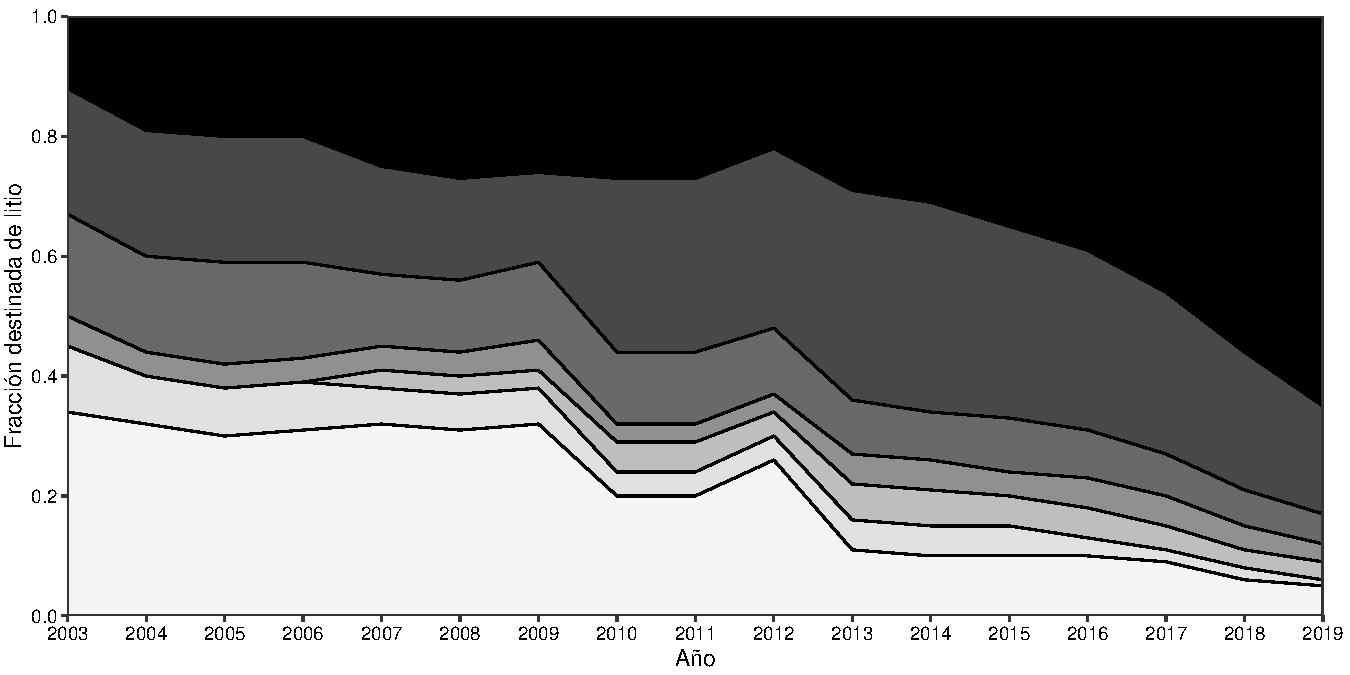
\includegraphics[width=0.986\textwidth,trim={0 0.85cm 0 0}, clip]{chap2/images/usesRel.pdf}}
               \put(2, 202){\large a)}
               \end{picture}}\\%
    \subbottom{\begin{picture}(500,230)
               \put(0, 0){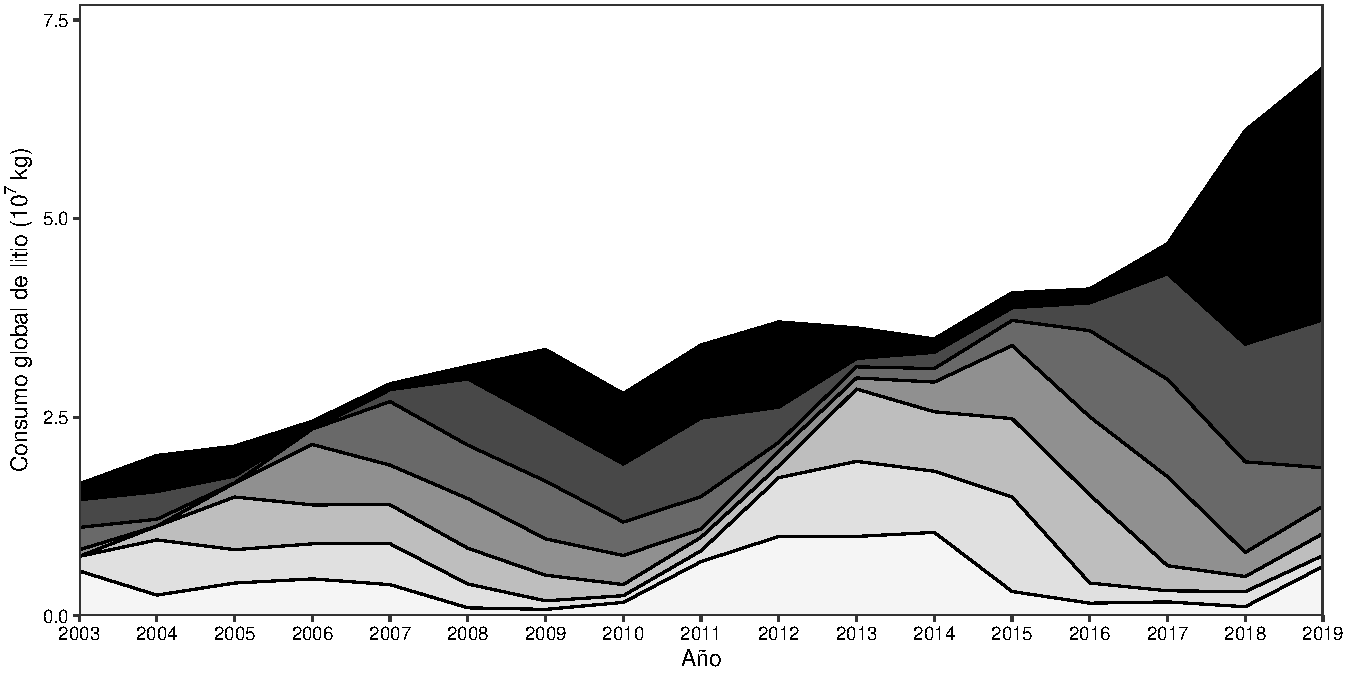
\includegraphics[width = \textwidth]{chap2/images/usesAbs.pdf}}
               \put(0, 223){\large b)}
               \end{picture}}
    \caption[Series de tiempo mercados finales de consumo de litio desde el año 2003.]{Mercados finales de consumo de litio desde el año 2003. (a) en proporción y (b) en cantidades absolutas. Las zonas del gris más oscuro al más claro corresponden a fabricación de baterías, mejoramiento de cerámicos y vidrios, fabricación de lubricantes, síntesis de polímeros, elaboración de polvos fundentes, tratamiento de aire, y otros usos (aleaciones con aluminio, uso farmacéutico, entre otros) respectivamente.  Elaborado con datos recolectados de \citet{    SQM2003, SQM2004, SQM2005, SQM2006, SQM2007, SQM2008, SQM2009, USGS2011, USGS2012, USGS2013, USGS2014, USGS2015, USGS2016, USGS2017, USGS2018, USGS2019}.}
    \label{fig:uses}
\end{figure}

La Figura \ref{fig:uses} contiene la serie de tiempo de la evolución del mercado final del litio producido en el mundo desde el año 2003. El mercado de baterías ha monopolizado más del 60\% del consumo global de litio, que solía estar distribuido más o menos con uniformidad entre diversas industrias. En la figura con escala absoluta (Figura \ref{fig:uses}(b)), puede observarse que en los últimos años la demanda de este sector aumenta casi constantemente. Esto responde al uso cada vez más dispositivos portátiles, que por lo general funcionan con energía almacenada en baterías de ion de litio \acused{LIB}(LIBs) y, principalmente, al mercado de los vehículos eléctricos \acused{EV}(EVs) que cada vez gana más protagonismo en medio de la tendencia global hacia la utilización de energías y tecnologías más limpias desde un punto de vista ambiental. Adicionalmente, en algunos escenarios se especula que las baterías con litio serán la opción predilecta para almacenar energía eléctrica proveniente de fuentes renovables cuando la quema de combustibles fósiles se haga obsoleta \citep{SVERDRUP2016}.

La relevancia de este elemento ha sido reconocida por organismos gubernamentales de distintos países. La Dirección General de Desarrollo Minero de la \citet{SecEc2018} habla de la importancia de este elemento, y menciona algunos de los potenciales yacimientos que podrían posicionar al país como una potencia mundial de este recurso. El Servicio Geológico de Estados Unidos (USGS) considera que el litio es un elemento crítico que podría hacer contribuciones importantes hacia la tan anhelada autonomía energética de ese país \citep{Bradley2017}. El Servicio Geológico Británico considera al litio en su \textit{lista de riesgo} de suministro de elementos y lo ubica al mismo nivel de importancia que los metales preciosos del grupo del platino \citep{STERBA2019416}. La Unión Europea no considera al litio como un elemento crítico, pero admite que su importancia crece constantemente \citep{European2018}.

El suministro mundial de litio puede ser suficiente para varias décadas por venir, pero su futuro encarecimiento y escasez es inevitable si la flota automotriz es reemplazada en su totalidad por vehículos de propulsión eléctrica \citep{SVERDRUP2016}. Una gran parte de los análisis prospectivos que abordan la dinámica de la demanda y la oferta de metales críticos para las próximas décadas, centran su atención al caso del litio incluso a expensas de que algunos otros metales, considerados como más críticos, están siendo ignorados en gran medida \citep{Watari2020}. Si la oferta mundial de litio llega a ser incapaz de satisfacer las necesidades del creciente sector transporte, se ralentizaría la migración masiva de este sector hacia el uso de energías más limpias \citep{VIKSTROM2013}. Algunos autores concluyen que en un futuro cercano el litio no es un cuello de botella para el suministro de las materias primas necesarias para la fabricación de \acp{LIB}, pero esto podría modificarse drásticamente obedeciendo cambios políticos o económicos que incentiven un crecimiento inesperado del sector de transporte eléctrico \citep{Olivetti2017}. En efecto, varios factores aceleran hoy por hoy el crecimiento de este sector. Un ejemplo radical lo presenta el Reino Unido de Gran Bretaña e Irlanda del Norte, cuyo gobierno ha impuesto un veto a la venta de vehículos de combustión e híbridos para el año 2035, y un veto a su circulación para el año 2050 \citep{BBC2020}.

Las \acp{LIB} son actualmente la mejor tecnología para el almacenamiento de energía eléctrica \citep{Zubi2018}. Su desarrollo entre 1970 y 1985 representó un aporte muy importante, por lo que los científicos John Goodenough, Stanley Whittingham, y Akira Yoshino fueron galardonados con el Premio Nobel de Química en el 2019 por los aportes realizados a su invención \citep{Royal2019}. Hoy en día, medio siglo después de los primeros avances en la materia, la investigación de materiales para la producción de baterías cada vez más robustas y eficientes continúa con ahínco. Por ejemplo, recientemente \citet{Harlow2019} reportaron una nueva \ac{LIB} de muy alto desempeño que podría funcionar en un auto eléctrico durante 1.6\e{6}~km, un orden de magnitud por encima de la longevidad promedio de los automóviles actuales.% Este desarrollo (patrocinado por Tesla Inc., el gigante de los autos eléctricos) ayuda a resolver uno de los mayores inconvenientes relacionados con el sector de la transportación impulsada por energía eléctrica. %\citep{Ford2012}.

% READ THIS!!!
% https://www.nobelprize.org/uploads/2019/10/advanced-chemistryprize2019-2.pdf
\clearpage
\subsection{Contexto geoeconómico}
Como en la mayoría de los elementos de la tabla periódica, la distribución del litio no es uniforme alrededor del mundo. Los mapas de las reservas y los recursos de litio por país se muestran en las Figuras \ref{fig:reservas} y \ref{fig:recursos}, respectivamente. Las reservas hacen alusión a cantidades probadas de un elemento, extraíbles de una manera económicamente viable. Los recursos hacen alusión a la estimación total de un elemento en un determinado territorio. La diferencia entre reservas y recursos viene dictaminada principalmente por la demanda de un elemento, ya que esta afecta el precio al cual se adquieren sus productos \citep{VIKSTROM2013}. 

Los mayores productores de litio actualmente son Australia y Chile. El litio de Australia es extraído de minerales que muchas veces son comercializados en forma de concentrados que requieren procesos cortos de beneficiación. Estos concentrados son usados directamente en la manufactura de cerámicos y vidrios \citep{Bradley2017}. El litio de Chile se encuentra en forma de minerales disueltos en lagos salados (i.e.\ salares).  Bolivia, Argentina y Chile son los países con los recursos de litio más grandes del mundo. Estos países definen el llamado {triángulo del litio} por la vasta cantidad de litio que tienen en sus salares. Mientras la extracción del litio de Bolivia no es viable económicamente hoy por hoy, Argentina es el cuarto productor de litio más importante \citep{USGS2020}. China tiene reservas importantes de litio y es el tercer productor más importante de este elemento. Sin embargo, el gigante asiático depende fuertemente de las importaciones debido a que por su alto nivel de industrialización consume cerca de la mitad del litio producido mundialmente cada año \citep{Olivetti2017}. 

Los recursos de litio más importantes del mundo se encuentran en los océanos, con un volumen total estimado de 1.37\e{9}~km$^3$ y una concentración promedio de ion litio de alrededor de 0.18~mg~kg\mnn\ \citep{KRESS20191, Evans2013, HOSHINO201311}. La cantidad de litio presente en este medio puede ser de alrededor de 250 millones de toneladas. Este valor es mucho mayor que las reservas combinadas de todos los países ricos en litio \citep{Yang2018}. En la actualidad, la extracción de ion litio a partir de agua de mar no es viable económicamente debido a su baja concentración y a la presencia de altos niveles de cationes que interfieren en su proceso de recobro. El costo de extracción de ion litio a partir de agua de mar es el más elevado y se encuentra en el extremo opuesto de una lista encabezada por el Salar de Atacama, en Chile, de donde el kilogramo de carbonato de litio equivalente\acused{LCE} (LCE)\footnote{El carbonato de litio equivalente es la terminología estándar usada en la industria del litio. 1~$kg$ de litio es equivalente a 5.323~$kg$ LCE.} se extrae a menos de 2 dólares estadounidenses (USD)\acused{USD} \citep{KUSHNIR2012}. A pesar de la no viabilidad económica de la extracción del ion litio presente en agua de mar, vale la pena anudar esfuerzos en el desarrollo de nuevas metodologías que permitan su recobro a partir de esta matriz porque hacia allá se puede volcar el mercado de extracción de ion litio cuando sus fuentes continentales, más rentables y menos complicadas, empiecen a escasear.

El precio de los compuestos principales de litio ha aumentado casi constantemente en los últimos años \citep{MARTIN2017}. En el 2019, en medio de la guerra comercial entre China y Estados Unidos, China redujo los generosos subsidios que estaba otorgando a compradores y fabricantes de \acp{EV} y esto produjo una sobreoferta de litio que repercutió en una disminución de su precio en casi un 25\% \citep{Kalantzakos2019}. Sin embargo, la popularidad de los \acp{EV} sigue en aumento, y la balanza de la oferta-demanda podría inclinarse nuevamente a favor de los países productores de litio en cualquier momento \citep{LIU2019}.

%https://sci-hub.tw/10.1016/j.watres.2019.01.050

% https://sci-hub.tw/10.1016/j.apenergy.2013.04.005

\begin{figure}[H]
    \centering
    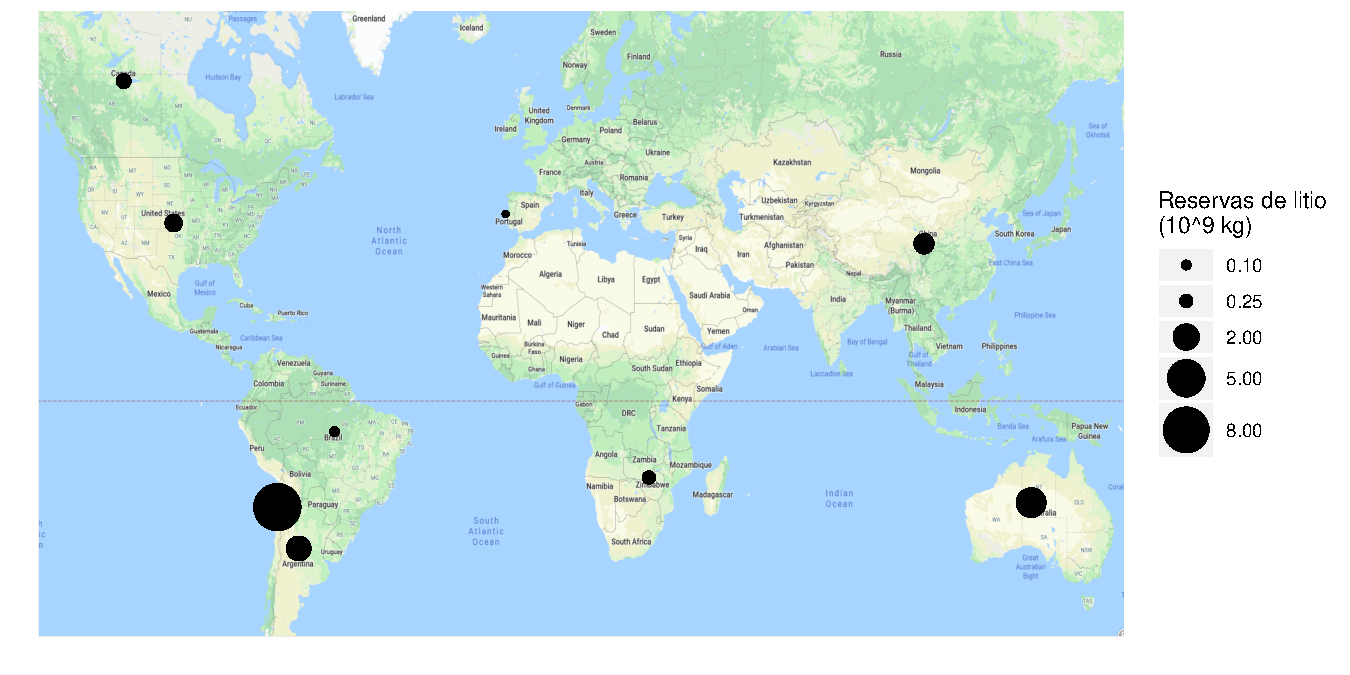
\includegraphics[width = \textwidth, trim = {1cm 1.2cm 0.4cm 0.5cm}, clip]{chap2/images/reserves.pdf}
    \caption[Reservas de litio por país.]{Reservas de litio por país. El diámetro de los círculos es proporcional a la cantidad de litio en millones de toneladas \citep{USGS2020}.}
    \label{fig:reservas}
\end{figure}
\begin{figure}[H]
    \centering
    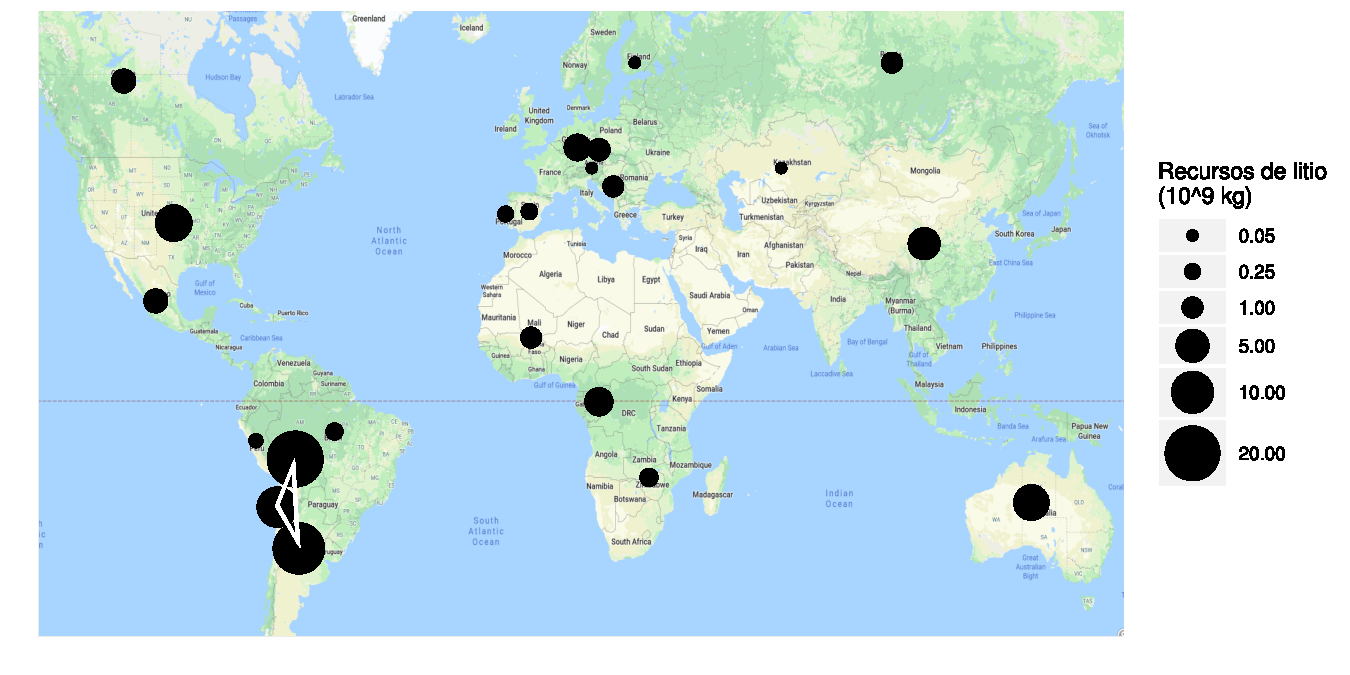
\includegraphics[width = \textwidth, trim = {1cm 1.2cm 0.4cm 0.5cm}, clip]{chap2/images/resources.pdf}
    \caption[Recursos de litio por país.]{Recursos de litio por país. El diámetro de los círculos es proporcional a la cantidad de litio en millones de toneladas \citep{USGS2020}. El {triangulo del litio} en Suramérica se señala con blanco.}
    \label{fig:recursos}
\end{figure}

\subsection{El litio de México}\index{Litio!Bacadéhuachi-Sonora}
%https://www.gob.mx/cms/uploads/attachment/file/419275/Perfil_Litio_2018__T_.pdf
%https://www.bacanoralithium.com/pdfs/Ni-43-101-Mineral-Resource-Estimate-For-The-Sonora-Lithium-Project-Mexico-May-2015.pdf
%https://www.bacanoralithium.com/pdfs/Bacanora-FS-Technical-Report-25-01-2018.pdf
México no figura entre los grandes productores de litio. Como puede observarse en la Figura \ref{fig:reservas}, el Servicio Geológico de Estados Unidos no contabiliza reservas en este país. % y la Figura \ref{fig:recursos} muestra que los recursos que le atribuyeron a México no llegan a las dos millones de toneladas. 
No hay proyectos de extracción de litio en fase de explotación comercial en territorio mexicano y las importaciones de este elemento involucran un negocio multimillonario que se encuentra exento de pagos arancelarios \citep{SecEc2018}. A pesar de esto, en un futuro cercano México podría sentarse en la mesa de las potencias del litio.

Se encuentran en etapa de exploración cerca de 11 proyectos de extracción de ion litio, de los cuales el más importante se encuentra en Bacadéhuachi, en el estado de Sonora, al norte del país. A esta locación se le atribuye ser actualmente el proyecto de explotación de litio más grande del mundo, con una exorbitante cantidad de más de 240 millones de toneladas de mineral con una concentración promedio de litio de 0.35\% en masa \citep{Bacanora2018}. Esta cifra ha sido muy mal utilizada por la prensa común, que irresponsablemente habla de {240 millones de toneladas de litio}.\footnote{Esto es equivalente a la cantidad total de litio presente en la vastedad de los océanos, el mayor reservorio de litio de nuestro planeta.} Esto puede conducir a la errónea conclusión de que México es, como ellos anuncian, la nueva Arabia Saudita del litio. La estimación real en el yacimiento es de cerca de un millón de toneladas extraíbles a un excelente costo total de producción de aproximadamente 4 \ac{USD}~kg$_{LCE}^{-1}$. Estas cifras son bastante prometedoras, y ubican al país como el cuarto o quinto con las mayores reservas de litio en el mundo. El yacimiento consta principalmente de arcilla de hectorita (ver Sección \ref{sec:arcillas}). Ya se encuentra en operación una planta piloto de refinamiento y purificación para la obtención de carbonato de litio de grado para baterías ($\geqslant$99.5\%). Se espera que la mina entre en operación en el 2022 \citep{Bacanora2018}.

% Tesla y Bocanora firmaron convenio para asegurar el suministro de litio al gigante de los EVs

%La zona del yacimiento de litio de Bacadéhuachi-Sonora es actualmente azotada por violencia de los carteles de narcotráfico y se le considera una región inestable. Resulta inevitable rememorar  los yacimientos de oro en el norte del País y el contexto de la fiebre del oro de California en la época de la injusta guerra México-Estados Unidos que cambió tan drásticamente el mapa de Norteamérica. Los tiempos han cambiado desde entonces. Casualmente, el litio ha sido denominado por muchos como oro/petroleo blanco \citep{Crooks2018} y el hecho de que el yacimiento se encuentre \textit{tan lejos de Dios y tan cerca de los Estados Unidos} (a menos de 300 km de la frontera México-Estados Unidos) puede tener poco que ver pues atravesar el océano atlántico no fue inconveniente para los Estados Unidos en el conflicto bélico con (su ex-aliado) Irak en la Segunda Guerra del Golfo para ocupar su territorio y disponer de sus recursos bajo un pretexto que nunca pudo ser demostrado. Sin embargo, una posible invasión suena muy inverosímil y los amados del neoliberalismo tienen herramientas más sutiles para despojar de sus recursos a los países que despectivamente han denominado \textit{tercermundistas}. El Gobierno de México debe pensar al respecto con calma y aparte de recordar siempre su historia para no tener que repetirla, puede aprender de algunos de los muchos errores de su \textit{Aliado del Pacífico},\footnote{La Alianza del Pacífico es un acuerdo de cooperación multilateral establecida en el 2011 por Chile, Colombia, México y Perú. El propósito es prosperar juntos y crear un bloque latinoamericano competitivo frente al mundo \citep{Prado2016}.} el Gobierno Colombiano, y evitar un detrimento irremediable de su Patrimonio Nacional.\footnote{En el año 2000, el Gobierno de Colombia vendió (regaló) su participación en la mina de carbón térmico bituminoso de alta calidad más importante de Latinoamérica, El Cerrejón. El evento coincidió con un alza pronunciada en el valor comercial de este recurso. Mientras en la zona de la mina se presencia pobreza extrema y un medio ambiente sumamente deteriorado, cada 4 horas salen locomotoras con más de $10^7$ kg de carbón que es vendido al mejor postor por parte empresas extranjeras que supieron, en el momento correcto, manipular y comprar a políticos endebles y corruptos que abundan en ese país sudamericano.}


%\subsection{Propiedades químicas}
\subsection{Principales fuentes de ion litio}\index{ion litio!fuentes}
Las principales fuentes de ion litio, sus compuestos más comercializados y el uso más común de los mismos se muestran en la Figura \ref{fig:esquemaSpiers}. Como se mencionó anteriormente, las reservas son fuentes extraíbles con procesos económicamente viables y los recursos incluyen todas las fuentes del elemento a pesar de la inviabilidad práctica de su extracción. A pesar de que el ion litio se encuentra presente en minerales, salmueras, arcillas y (principalmente) en agua de mar, la extracción a gran escala solo se hace actualmente partir de minerales (rocas), y salmueras. Con el éxito de las minas como las de Sonora en México, las arcillas pueden pasar a formar parte importante de las fuentes comerciales de este elemento. Ya se encuentran en operación plantas piloto para la producción de carbonato de litio a partir de arcillas y producen litio a precios muy competitivos \citep{Bacanora2018}.

Los procesos extractivos industriales pueden compartir características generales para fuentes de la misma naturaleza, pero las metodologías aplicables a un determinado yacimiento dependen en gran medida de las particularidades que presentan los recursos de dicho yacimiento. De esta manera, un proceso hidrometalúrgico diseñado para extraer ion litio de un salar en China puede no funcionar apropiadamente si se aplica sin modificaciones importantes a la extracción de ion litio de un salar en Bolivia.

{\floatstyle{boxed}
\restylefloat{figure}
\begin{figure}[H]
    \centering
    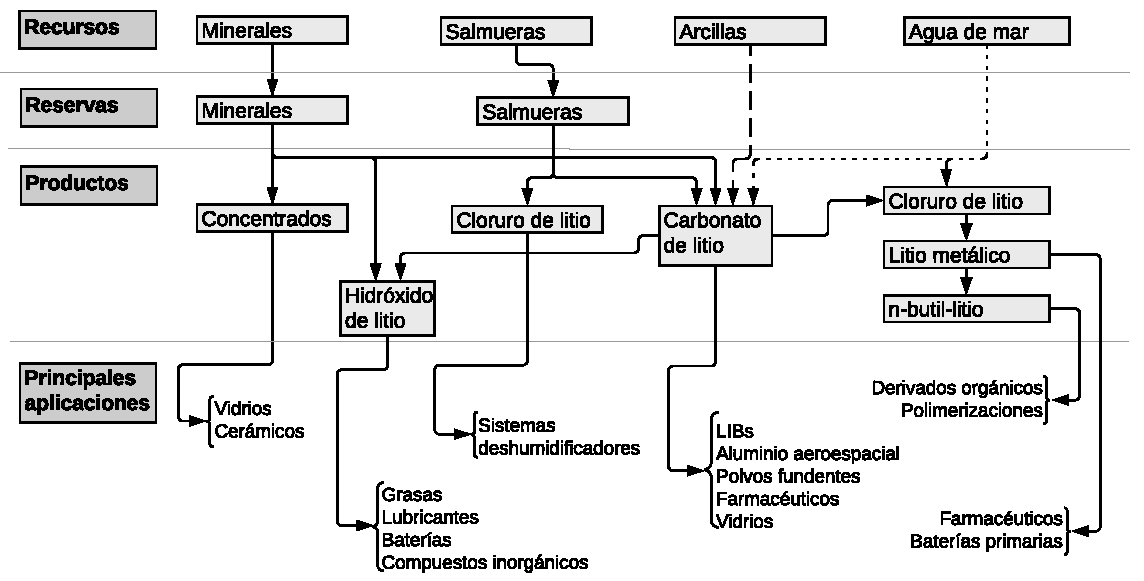
\includegraphics[width=\textwidth]{chap2/images/lithiumsoourcetoeum.pdf}
    \caption[Principales rutas del litio desde la fuente hasta su uso final.]{Principales rutas del litio desde la fuente hasta su uso final. Adaptado principalmente de \citet{SPEIRS2014}. La línea discontinua que desprende de arcillas es considerando el éxito de de proyectos como el de Bacadéhuachi-México y las líneas punteadas que desprenden de agua de mar son considerando la posible aplicación del presente proyecto.}
    \label{fig:esquemaSpiers}
\end{figure}
}

\subsubsection{Minerales en roca}\label{sec:pegma}
Los minerales de litio más relevantes se muestran en la Tabla \ref{tab:minerals} \citep{Anthony1995}. Estos minerales se presentan por lo general en forma de pegmatitas.\footnote{Rocas ígneas filolianas con intrusiones cristalinas} Las pegmatitas constituyen actualmente la mayor fuente de litio. Las minas más grandes de pegmatitas con litio están localizadas en Australia. La extracción del litio presente en esta matriz requiere inicialmente la destrucción del mineral por métodos mecánicos o químicos que demandan mucha energía y con frecuencia aumentan el costo de la extracción \citep{CHRISTMANN2015}.

\begin{table}[ht]
    \centering\footnotesize
    \begin{tabular}{@{}llrp{7cm}@{}}\toprule
        \textbf{Mineral} & \textbf{Fórmula empírica} & \textbf{Li (\%)} & \textbf{Detalles} \\\midrule
        Espomudena & \ce{LiAl(SiO3)2}      & 3.73 & Principal fuente mineral de litio.\\
        Lepidolita & \ce{KLi2AlSi4O10F(OH)}& 3.58 & Mineral de litio más abundante. Segunda fuente mineral más importante.\\
        Petalita   & \ce{LiAlSi4O10}       & 2.09 & Puede convertirse en Espomudena de alta calidad para su uso directo en cerámicos.\\
        Ambligonita& \ce{Li_{0.75}Na_{0.25}Al(PO4)F_{0.75}(OH)_{0.25}} & 3.44& Algunos yacimientos presentan hasta 10\% en masa de ion litio pero no es una fuente comercial importante por su baja abundancia.\\\bottomrule
    \end{tabular}
    \caption{Principales minerales (en roca) de litio.}
    \label{tab:minerals}
\end{table}

El mineral más importante de esta familia es la espomudena, cuyos concentrados pueden ser utilizados directamente como aditivo en vidrios y cerámicos, el segundo mercado final más importante del litio. Los concentrados son el resultado del beneficio de los minerales. Este proceso por lo general se realiza por medios mecánicos como flotación con líquidos densos y separación magnética \citep{TADESSE2019}. 

Para obtener compuestos de litio, el concentrado de mineral debe ser {tostado} a altas temperaturas en presencia de algún aditivo para formar compuestos lixiviables. Posteriormente el litio se concentra con resinas de intercambio iónico. Si se usa como aditivo, por ejemplo, ácido sulfúrico, se forman sales de sulfato que son lixiviables con agua caliente. Al elevar el pH del lixiviado acuoso, se eliminan por precipitación una parte importante de los cationes interferentes. La carbonatación de la disolución produce carbonato de litio, el compuesto más comercial de este elemento \citep{TRAN2015}.

\subsubsection{Salmueras}
Las salmueras de los salares componen actualmente los recursos más abundantes de litio. Los lagos salados con mayor cantidad de ion litio se encuentran en el triángulo del litio (ver Figura \ref{fig:recursos}), formado por Bolivia, Argentina y Chile. La concentración de ion litio en las salmueras de importancia comercial se encuentra entre 200 y 4000~mg~kg\mnn. La extracción del litio presente en estas matrices presenta la ventaja de que el elemento ya se encuentra en disolución y ya no son necesarias algunas de las etapas que consumen más energía cuando el litio se extrae a partir de minerales sólidos.

La obtención de compuestos de litio requiere inicialmente la eliminación de una porción importante del disolvente (agua), para concentrar el ion litio en el medio. Usualmente esto se hace por evaporación solar o por ósmosis inversa \citep{Swain2017}. El protocolo empleado en cada salmuera es diferente porque depende de las características del yacimiento. Si la salmuera contiene boro, este por lo general se retira con extracción por disolventes, porque el ácido bórico es un subproducto con valor comercial y porque el boro daña los sistemas de obtención de litio metálico a partir del cloruro de litio \citep{TRAN2015}. Los iones calcio y magnesio deben ser retirados por preci\-pi\-tación y posteriormente puede carbonatarse la disolución para precipitar carbonato de litio que posteriormente es purificado por recristalización o por filtración.

\subsubsection{Minerales en arcilla}\label{sec:arcillas}
Las  arcillas no son actualmente una fuente importante de litio, pero la situación promete cambiar próximamente con el avance de megaproyectos mineros ubicados principalmente en México y Estados Unidos. Las arcillas de litio más representativas se muestran en la Tabla \ref{tab:clays}. La más importante de este grupo es la hectorita. El proceso de extracción de litio a partir de estas matrices es similar al aplicado para obtener compuestos de litio a partir de rocas pegmatiticas.

\begin{table}[H]
    \centering\footnotesize
    \begin{tabular}{@{}llr@{}}\toprule
        \textbf{Mineral} & \textbf{Fórmula empírica} & \textbf{Li (\%)}\\\midrule
        Hectorita & \ce{Na_{0.3}(Mg,Li)_3Si_4O_{10}(OH)_2}  & 0.54 \\
        Jadarita & \ce{(Na,Ca)_{0,3(}Al,Mg)_2Si_4O_{10}(OH)_2.n(H_2O)}& -\\
        Polilitionita   & \ce{KLi_2AlSi_4O_10(F_{0.75}(OH)_{0.25})_2}       & -\\\bottomrule
    \end{tabular}
    \caption{Principales minerales (en arcillas) de litio.}
    \label{tab:clays}
\end{table}

El proceso de beneficio de las arcillas involucra un proceso de molienda fina y clasificación por tamaño de partícula usando un hidrociclón. Los aditivos añadidos en el tueste del concentrado son principalmente sulfato de sodio, sulfato de calcio (yeso) y carbonato de calcio (calcita). Se produce sulfato de litio que puede tratarse como se describió en la Sección \ref{sec:pegma} \citep{Bacanora2018}. Como subproducto de valor comercial se suele obtener sulfato de potasio.

\subsubsection{Agua de mar}
El ion litio se encuentra disuelto en el agua de mar a una concentración promedio de 0.18~mg~kg\mnn\ \citep{Evans2013}. Su concentración es diminuta, pero es el decimocuarto elemento más abundante en esta matriz. Como se ha mencionado en secciones anteriores, los océanos contienen el recurso de ion litio más grande conocido del planeta, y constituyen una fuente casi inagotable de este elemento \citep{Yang2018}; sin embargo, su extracción a escala industrial es inviable económicamente a causa de su baja concentración. Distintas metodologías son estudiadas actualmente para extraer ion litio a partir de esta matriz, pero se encuentran en etapa de investigación y desarrollo, por lo que se han incluido en la Sección \ref{sec:estadodelarte}.

\subsubsection{Reciclaje}

Actualmente, las cantidades de ion litio obtenidas por reciclaje no son importantes y puede que este panorama no cambie en un futuro próximo \citep{Olivetti2017}. El ion litio utilizado en cerámicos y vidrios no se puede recuperar \citep{CHRISTMANN2015}, y la minería urbana de \acp{LIB} por lo general se enfoca en la recuperación de cobalto o manganeso que tienen un mayor valor comercial. 

Algunas estimaciones establecen que para el 2050 el 25\% de la producción mundial de litio podría provenir de fuentes recicladas involucrando principalmente \ac{LIB}s. Este aumento del porcentaje sería en respuesta a la introducción al mercado masivo de baterías de ion litio de gran tamaño para \ac{EV}s, con el consecuente gran volumen de residuos que pueden representar dichas baterías hacia el final de su tiempo de vida útil (cerca de una década) \citep{STERBA2019416, Evans2013}. Predicciones sobre el crecimiento de la flota de vehículos eléctricos estiman que tan solo en los Estados Unidos podrían producirse hasta cuatro millones de toneladas de residuos de \ac{LIB}s en las próximas dos décadas \citep{RICHA2014}. 

Las \ac{LIB}s tienen entre 100 y 345~g de litio por cada kilowatt hora de capacidad. Esto representa cerca de 4~kg de litio en la batería de cada \ac{EV}. La dificultad principal que presenta el reciclaje del litio de estas fuentes recae en que la química de los cátodos empleados es muy variada (Tabla~\ref{tab:catodos}), y la minería urbana de este recurso se puede hacer menos eficiente dado que cada material requiere condiciones distintas de tiempo y composición, para la lixiviación eficiente de ion litio \citep{VENKATRAMAN2004}.% Políticas estrictas deberán establecerse para regular la recolección y clasificación de las baterías que han terminado su ciclo de vida.
\begin{table}[H]
    \centering\footnotesize
    \begin{tabular}{@{}p{3cm}lcp{5cm}@{}}\toprule
        \textbf{Nombre} &\textbf{Fórmula} &  \textbf{Energía específica}&\textbf{Detalles}\\
        &&(W~h~kg\mnn)\\\midrule
        Óxido de litio y cobalto (LCO) & \ce{LiCoO2} & 110-200 & Primer cátodo de uso industrial en \ac{LIB}s. Presenta desventajas de seguridad y ambientales, por riesgo de explosión y por el uso de cobalto, respectivamente.\\
        Óxido de litio, niquel, manganeso y cobalto & \ce{Li(Ni_{0.33}Mn_{0.33}Co_{0.33})O2} & 95-130 & Amplio uso en vehículos eléctricos.\\
        Espinela de litio y manganeso & \ce{LiMn2O4} & 110-120 & Bajo costo de producción. Amplio uso en vehículos híbridos eléctricos.\\
        Fosfato de litio y hierro & \ce{LiFePO4} & 95-140 & Es de los cátodos más seguros, con los menores costos de producción y con un bajo impacto negativo al medio ambiente\\\bottomrule
    \end{tabular}
    \caption[Principales materiales de los cátodos de LIBs.]{Principales materiales de los cátodos de \ac{LIB}s \citep{Chagnes2015}}
    \label{tab:catodos}
\end{table}

\subsection{Problemas socio-ambientales asociados}
El litio permite el funcionamiento de diversas tecnologías que prometen ayudar a disminuir el impacto ambiental negativo que acarrean muchas de las actividades humanas. A pesar de esto, su extracción y utilización no está libre de consecuencias para algunos de los ecosistemas y las poblaciones que rodean los yacimientos importantes.

El ejemplo más notorio lo presenta la extracción del ion litio presente en el Salar de Atacama en Chile, parte del triángulo del litio. La evaporación de grandes cantidades de agua de los salares para aumentar la concentración de ion litio resulta catastrófica para la fauna del lugar, porque el Desierto de Atacama es un lugar extremadamente seco y el acceso a las fuentes hídricas se encuentra injustamente restringido a su aprovechamiento comercial. Los reservorios subterráneos de estos salares son alimentados por fuentes acuáticas que también alimentan lagos que son muy importantes para las regiones circundantes. La minería de litio en esta región compite con los pobladores por el uso del agua y en los últimos  censos nacionales se ha evidenciado una caída importante en su población \citep{Romero2012, LIU202012}.

Por otro lado, el Salar de Uyuni, en Bolivia, es el segundo reservorio más grande conocido de ion litio (después de los océanos) con una excepcional estimación de 20 millones de toneladas de ion litio. Una dificultad importante que presenta la extracción de ion litio de este salar es que el ecosistema es muy delicado y el proyecto representaría una amenaza importante a la biodiversidad de la zona \citep{Hancock2018}. La protección de las especies endémicas de la región y de los pueblos indígenas que habitan la zona son un factor importante que afortunadamente han ralentizado el inicio de la explotación de este recurso.

Cuando la extracción de ion litio se hace a partir de rocas y arcillas, los procesos de calcinación y tueste tienen un gran impacto negativo al ambiente porque demandan altas cantidades de energía, liberan grandes volúmenes de emisiones atmosféricas, e involucran el uso de grandes cantidades de ácido \citep{Hancock2018}.

Los problemas sociales y ambientales de la extracción de ion litio a partir de agua de mar pueden ser significativamente menores que los asociados a los procesos de recobro a partir de salmueras y minerales rocosos o arcillosos. La cuasi-omnipresencia de los océanos permitiría ubicar los puntos de extracción en lugares donde el ecosistema sea robusto y no haya afectación a poblaciones humanas.

Respecto a los productos finales de litio, la fabricación de una batería con 1~kWh de capacidad requiere la inversión de cerca de 380~kWh de energía y el proceso puede liberar hasta 80~kg de \ce{CO2} \citep{Chagnes2015}. Al final de su ciclo de vida, estas baterías son consideradas residuos peligrosos que representan un peligro para el medio ambiente y para la salud de los humanos debido a sus altos contenidos de cobre, cobalto y níquel \citep{Kang2013}. El impacto negativo de estos residuos se mitigaría considerablemente con la implementación de políticas estrictas referentes al reciclaje de estos recursos.



\section{Estado del arte en el recobro de ion litio}\label{sec:estadodelarte}
Un gran número de metodologías se han propuesto para la separación selectiva de ion litio. En muchos casos los métodos han sido exitosamente aplicados a muestras reales, incluyendo agua de mar. En esta sección se resumen aspectos relevantes de estas técnicas. Las \acp{PIM} son tratadas independientemente en la Sección \ref{sec:pimint}.

La Tabla \ref{tab:ArtLitreports} resume algunos de los métodos recientes para la extracción de ion litio a partir de distintas matrices. De las técnicas incluidas, adsorción, intercambio iónico y electrólisis selectiva no comparten muchas características con el método propuesto en el presente trabajo. Por otro lado, la extracción con disolventes y con membranas líquidas soportadas contienen conceptos fácilmente adaptables a las \acp{PIM}. Este segundo grupo es analizado con más detalle en los siguientes apartados.

\clearpage
%\newgeometry{left=1cm, bottom=0.4cm, top=0.16cm}
\begin{landscape}%\thispagestyle{plain}
\centering
\begin{table}[H]
    \centering\footnotesize
    \begin{tabular}{@{}p{0.07cm}llcp{12cm}l@{}}\toprule
        &\textbf{Material o Reactivo} &\textbf{Matriz}&\textbf{Eficiencia}&\textbf{Detalles}&\textbf{Referencia} \\&&&\textbf{(\%)}\\\midrule
        \multicolumn{3}{@{}l}{\textit{Extracción con disolventes}}\\
        &LIX-54/Cyanex 923&Sintética&98&\textbf{Rel. mol.}: 2:1 (LIX-54:Cyanex 923). \textbf{Dil}: ShellSol D70 (Parafinas y naftenos C11-C14).\newline Efecto sinérgico entre los extractantes. & \citet{Pranolo2015}\\
        &LIX-54/TOPO & Sintética &- & \textbf{Dil}: Queroseno.\newline Efecto sinérgico entre los extractantes.  &\citet{Kunugita1989}\\
        &TTA/TOPO & Agua de mar & 65& \textbf{Dil}: Queroseno.\newline Efecto sinérgico entre los extractantes. El magnesio fue precipitado con \ce{NH4OH}. & \citet{Harvianto2016}\\
        &\ce{[N4444][EHEHP]}&Sintética&95& \textbf{Dil}: Dicloroetano.&\citet{Shi2020}\\
        &TBP&Sintética&65& \textbf{Dil}: Succinato de dietilo. \textbf{Cox}:\ce{FeCl3}. &\citet{Zhou2020}\\
        
        \multicolumn{3}{@{}l}{\textit{Membranas líquidas Soportadas}}\\
        &LIX-54/TOPO& Sintética&90&\textbf{Rel. mol.}: 3:1 (LIX-54:TOPO). \textbf{Dil}: Queroseno. \textbf{Rec}: \ce{H2SO4} (1~mol~L\mnn)&\citet{Ma2000}\\
        &D2EHPA/TBP & Sintética&82&\textbf{Dil}: Queroseno. \textbf{Rec}: \ce{HCl}  &\citet{sharma2016}\\
        &\ce{[C4mim][NTf2]}/TPB& Sintética &70 & \textbf{Pol}:  poli(1,1-difluoroetileno). \textbf{Rec}: \ce{Na2CO3 + NaHCO3} (2~mol~L\mnn)&\cite{ZANTE2019}\\
        
        \multicolumn{3}{@{}l}{\textit{Adsorción e intercambio iónico}}\\
        &\ce{H_{1.6}Mn_{1.6}O4}&Agua de mar &85&\textbf{Cap}: 40~mg~g\mnn&\citet{Chitrakar2001}\\
        &\ce{H_{1.33}[Ti_{x}Mn_{1-x}]_{1.67}O4}&Agua de mar&-&\textbf{Cap}: 22~mg~g\mnn &\citet{RYU2019}\\
      %  &HMO/Celulosa& & &\citet{Tang2020}\\
        
        \multicolumn{3}{@{}l}{\textit{Métodos electroquímicos}}\\
        &\ce{[PP13][NTf2]}&Agua de mar & -&Electrólisis de membrana líquida soportada con líquido iónico como extractante.&\citet{Hoshino2014}\\
        &LISICON& Agua de mar & - & Electrólisis de membrana selectiva a litio (LISICON)\newline Obtención directa de litio metálico. La celda funciona con energía solar. &\citet{Yang2018}\\
        &CEM/BLM/CEM& Sintética & 49 &\textbf{Rec}: HCl (0.03~mol~L\mnn)\newline Electrólisis de membrana líquida (TBP) intercalada entre dos CEMs &\citet{ZHAO2020}\\
        
        
        
        \multicolumn{3}{@{}l}{\textit{Membranas poliméricas de inclusión}}\\
        &TTA/TOPO & Sintética & &\textbf{Rel. mol.}:  2:1 (TTA:TOPO). \textbf{Rec}: HCl (0.1~mol~L\mnn)\newline La membrana pierde el 64\% de su eficiencia tras el cuarto ciclo de reuso.   &\citet{Cai2019}\\
        &\textbf{LIX-54/Cyanex 923} & \textbf{Agua de mar} &  &\textbf{Rel. mol.}: 2.15:1 (LIX-54:Cyanex 923)  \textbf{Rec}: HCl (0.1~mol~kg\mnn) \newline La membrana pierde menos del 40\% de su eficiencia tras el décimo ciclo de reuso.&\textbf{Este trabajo}\\\bottomrule   
        
       \multicolumn{6}{@{}p{23.5cm}@{}}{\scriptsize 
        \textbf{LIX-54}: 1-fenildecanona-1,3-diona. \textbf{Cyanex 923}: Mezcla de óxidos de trialquil fosfinas. \textbf{TOPO}: Óxido de trioctilfosfina. \textbf{TTA}: Teonil trifluoroacetona.          \textbf{\ce{[N_{4444}][EHEHP]}}: 2-etilhexilhidrogeno-2-etilhexilfosfonato de tetrabutilamonio.
        \textbf{TBP}: Tributilfosfato. \textbf{D2EHPA}: Ácido Di-(2-etillhexil)fosfórico.       \textbf{\ce{[C4mim][NTf2]}}: bis(trifluorometilsulfonilimida) de 1-butil-3-metilimidazolio. \textbf{\ce{[PP13][NTf2]}}:  bis(trifluorometilsulfonilimida) de N-metil-N-propilpiperidinio. %\textbf{HMO}: Óxido metálico con hidrógeno.  
        \textbf{LISICON}: Membrana superiónica conductiva de litio. \textbf{CEM}: Membrana de intercambio catiónico.\newline \textbf{BLM}: Membrana líquida \textit{de bulto}.
        \newline\textbf{Rel. mol.}: Relación molar de extractantes.
        \textbf{Dil}: Diluente de los extractantes. 
        \textbf{Cox}: Agente de coextracción.
        \textbf{Pol}: Polímero soporte. 
        \textbf{Rec}: Fase receptora o de recuperación. 
        \textbf{Cap}: Capacidad específica de adsorción de litio}
    \end{tabular}
    \caption{Métodos del estado del arte en extracción de litio.}
    \label{tab:ArtLitreports}
\end{table}
\end{landscape}

\subsection{Extracción con disolventes}\label{sec:extr.disolv}\index{Extracción!con disolventes}
La extracción con disolventes (o extracción líquido-líquido) se fundamenta en el reparto preferencial de un soluto entre dos fases líquidas inmiscibles que se encuentran en contacto. El reparto preferencial de dicho soluto en una fase o la otra depende en parte de la solubilidad que este presenta en cada uno de los medios. Con regularidad se emplean disolventes orgánicos para extraer cationes metálicos que se encuentran en medio acuoso. La solubilidad de estos solutos es bastante baja en el medio orgánico debido a la naturaleza de los cationes y de los disolventes orgánicos. Debido a esto, usualmente se incorporan en la fase orgánica extractantes orgánicos que forman compuestos estables neutros con los cationes y favorecen su reparto. Esto se conoce como extracción facilitada. En un segundo paso, el proceso es revertido usando una nueva disolución acuosa a partir de la cual, en pasos posteriores, pueden obtenerse compuestos de alta pureza del elemento en cuestión \citep{NARBUTT2020}. La primera disolución acuosa que contiene originalmente la especie de interés es denominada fase donadora o de alimentación, mientras la segunda se llama fase receptora o de recuperación. Las etapas de la separación se conocen como extracción y recuperación, respectivamente. Las condiciones de la extracción pueden ser finamente ajustadas a tal punto que incluso se hace posible la separación isotópica de distintos elementos. \citet{LIU2018c} reportaron el uso de éteres corona para la separación isotópica de \ce{^6Li}. Este isótopo es de gran importancia para la producción de tritio (\ce{^3H}) que se emplea en algunos reactores nucleares.

Los extractantes \index{Extractantes} que facilitan la extracción pueden dividirse en tres grupos principales, acorde al mecanismo de interacción con la especie que se extrae:
\begin{itemize}
    \item Extractantes ácidos (intercambiadores catiónicos)
    \item Extractantes alcalinos (intercambiadores aniónicos)
    \item Extractantes neutros (agentes solvatantes)
\end{itemize}

Los extractantes alcalinos son útiles en la extracción de especies con carga negativa. El ion litio no forma compuestos aniónicos bajo las condiciones del presente estudio, por lo que estos extractantes no son de interés en este trabajo.

En los extractantes ácidos (representados como \ce{HL}), la especie de interés (\ce{M^n+}) desplaza protones ácidos que son donados al medio acuoso para formar un complejo neutro (\ce{ML_n}), que por lo general es soluble en la fase orgánica:
\begin{equation}
    \ce{M^{n+} + n\overline{HL} <=> \overline{ML_n} + nH^+}
\end{equation}
donde la barra horizontal superior denota que la especie se encuentra en la fase no acuosa. 

Los agentes quelantes (\ce{B}), involucran la complejación de especies neutras (\ce{MX_n}) para formar un complejo también neutro (\ce{MX_nB_b}) que es altamente soluble en la fase orgánica:
\begin{equation}
    \ce{M^{n+} + nX^{-} + b\overline{B} <=> \overline{MX_nB_b}}
\end{equation}
En varios casos, los extractantes ácidos pueden reaccionar con el catión de interés como intercambiador catiónico y como agente solvatante, de manera simultánea \citep{Swain2016}:
\begin{equation}
    \ce{M^{n+} + (n + m)\overline{HL} <=> \overline{ML_n(HL)_m} + nH^+}
\end{equation}

La extracción de ion litio utilizando únicamente extractantes neutros es difícil, por lo que usualmente se requiere la adición de un anión anfifilico\footnote{Afín a ambas fases: acuosa y orgánica.} que permita la posterior solvatación del par iónico formado, por parte de la molécula extractante. \citet{Zhou2020} reportaron la utilidad del cloruro de hierro(III), que en medio acuoso con cloruros forma el complejo tetracloroferrato(III), para facilitar la solvatación de ion litio, usando un extractante orgánico neutro (TBP).

Un enfoque común para la extracción de cationes metálicos consiste en la combinación de un extractante ácido con uno neutro. La combinación de estos extractantes puede dar lugar a procesos que son más eficientes que la suma de las eficiencias de los procesos realizados con dichos extractantes de manera individual.  Esto se conoce como efecto sinérgico y ha sido ampliamente aplicado a la extracción de ion litio \citep{Pranolo2015, Kunugita1989, Harvianto2016}. La dificultad que presentan los extractantes ácidos para extraer por sí mismos al ion litio recae en que su número de coordinación es de cuatro \citep{Kinugasa1994}, y el extractante no satisface las necesidades de coordinación del ion litio. Los espacios remanentes son ocupados con moléculas de agua, formando una esfera de hidratación que hace el complejo incompatible con la fase orgánica altamente hidrofóbica. Estos espacios disponibles en el compuesto neutro formado por la base conjugada del extractante ácido y el ion litio, pueden ser ocupados por un agente quelante lipofílico que permita la incorporación del compuesto final a la fase orgánica \citep{NARBUTT2020}.

En algunos casos, la extracción con disolventes es aplicada para la extracción de los cationes calcio y magnesio que impiden la precipitación de compuestos de litio de alta pureza \citep{Shi2020b}. Este enfoque es ventajoso desde un punto de vista práctico, dado que los cationes divalentes son solvatados con mayor fuerza que los cationes monovalentes y, por lo tanto, su proceso de extracción es más rápido y sencillo.

\subsection{Membranas líquidas soportadas}\index{Extracción!con membranas líquidas soportadas}
Una membrana es una barrera física semipermeable que separa dos medios. Las membranas líquidas pueden ser soportadas (membrana líquida soportada (SLM)\acused{SLM}) o no soportadas (como las membranas líquidas de bulto (BLM) \acused{BLM}). Las \ac{SLM}s consisten en un soporte polimérico poroso impregnado con un disolvente orgánico que incorpora las moléculas extractantes. El uso de estas membranas representa una evolución de la extracción por disolventes y resuelve bastantes problemas relacionados con dicha metodología. Las etapas de extracción y de recuperación se llevan a cabo simultáneamente en un proceso que involucra cantidades de disolventes y de extractantes mucho menores a los usados en la extracción con disolventes. Esto representa ventajas operacionales y ambientales muy grandes. Su versatilidad las hace muy atractivas para distintas aplicaciones. Numerosas separaciones de iones metálicos han sido logradas usando este tipo de membranas \citep{deGyves1999}.

La separación de iones metálicos por medio de \ac{SLM}s puede lograrse con la adaptación de sistemas de extractantes y disolventes previamente reportados en la extracción con disolventes para el ion de interés. \citet{Ma2000} usaron en una \ac{SLM} los mismos extractantes diluidos en el mismo disolvente del sistema de extracción por disolventes reportado por \citet{Kunugita1989}. Los efectos sinérgicos entre extractantes ácidos y neutros reportados en la extracción de ion litio por disolventes, también son posibles (y muchas veces, necesarios) en la extracción usando \ac{SLM}s.

El principal inconveniente que presentan las \ac{SLM}s reside en la poca estabilidad que presentan a causa de fenómenos como emulsión de la fase orgánica en las fases acuosas, o volatilización del disolvente que diluye los extractantes. Estos inconvenientes pueden ser subsanados con el uso de líquidos iónicos como extractantes \citep{ZANTE2019}, o modificando la estrategia de la separación, usando otro tipo de membranas más estables, como las membranas poliméricas de inclusión.

La mayoría de los parámetros de desempeño relacionados con las \ac{SLM}s son comunes con los de las \acp{PIM} y por lo tanto, son tratados en la siguiente sección.
%\subsection{Métodos electroquímicos}
%\citep{Yang2018} LESS: 7828220525
%\citep{ZHAO2019}

%\subsection{Adsorción selectiva}
%Recovery of lithium in seawater using a titanium intercalated lithium manganese oxide composite
%Author links open overlay panelTaegongRyu
%10.1016/j.hydromet.2018.12.012


%\subsection{Adsorción selectiva e intercambio iónico}
%Recurrentemente se han estudiado materiales sólidos con alta selectividad hacia el litio para la separación selectiva de este elemento a partir de salmueras y de agua de mar \cite{ARROYO2019}. Los materiales más utilizados son óxidos metálicos (principalmente de manganeso) que capturan selectivamente iones litio en su estructura cristalina o resinas de intercambio catiónico en las que el litio reemplaza posiciones ocupadas por iones hidronio. En muchos casos los adsorbentes y las resinas empleadas se encuentran disponibles comercialmente.

%El protocolo involucra el contacto íntimo entre la disolución con litio (disolución de alimentación) y el adsorbente o la resina de intercambio iónico. Cuando el material sólido se ha cargado con litio al máximo de su capacidad se lava y se repite el proceso de contacto íntimo usando esta vez una disolución de recuperación generalmente compuesta de ácido clorhídrico diluido. En la segunda etapa, el litio es retirado del material sólido con lo que éste es regenerado y puede usarse nuevamente. Si se reutiliza la disolución de recuperación o si el volumen empleado es menor al de la disolución de alimentación puede concentrarse el litio y esto facilita la posterior obtención de compuestos sólidos.

%Algunas variaciones involucran los materiales sólidos para retirar del medio a todos los cationes exceptuando al litio que queda en disolución. \citet{Nishihama2011} reportaron el uso secuencial de resinas de intercambio iónico para eliminar los cationes alcalinos y alcalinotérreos que podrían interferir en la precipitación de litio a partir de un concentrado de agua de mar. Luego de eliminar los interferentes el litio pudo ser precipitado usando carbonato de amonio para obtener carbonato de litio con una pureza mayor a 99.9\%.

%\subsection{No se como llamar lo de acá D:0\}}
%Innovative lithium recovery technique from seawater by using world-first dialysis with a lithium ionic superconductor
%https://doi.org/10.1016/j.desal.2014.12.018





\section{Membranas poliméricas de inclusión}\label{sec:pimint}\index{PIM}
Las membranas poliméricas de inclusión (PIM) son un tipo de membranas líquidas que incorporan extractantes en la red polimérica de un termoplástico no poroso. Las \ac{PIM}s tienen las ventajas que presentan las \ac{SLM}s (unificación de los pasos de extracción y recuperación, bajo consumo de extractantes y de disolventes), y superan el principal inconveniente de este tipo de membranas relacionado con su pobre estabilidad \citep{Nghiem2006}. A diferencia de las SLM, en una PIM los extractantes no se encuentran disueltos en un disolvente que está impregnado en los canales de una membrana porosa, sino que se encuentran absorbidos en la red polimérica por fuerzas capilares y de unión no covalente. Dado que los extractantes no se encuentran en contacto tan directo con las disoluciones acuosas, son más resistentes frente a la lixiviación. 

Las \ac{PIM}s se encuentran en aplicaciones que van más allá de la separación selectiva de especies en disolución. Han sido utilizadas en distintas técnicas analíticas de cuantificación de especies (por métodos electroquímicos y espectrofotométricos), y de pretratamiento de muestras (preconcentración de especies y muestreo pasivo) \citep{ALMEIDA2017}. La separación selectiva de especies en disolución utilizando PIMs puede ser con fines extractivos, o para disminuir la peligrosidad de residuos mineros, industriales, y nucleares \citep{Kolev2019}.

El polímero base generalmente es de triacetato de celulosa (CTA) \acused{CTA} o de poli(cloruro de vinilo) (PVC) \acused{PVC}. El polímero se encarga de dar forma a la membrana y de proveerle resistencia mecánica. En la mayoría de los casos, se hace necesaria la adición de un plastificante que provee flexibilidad al polímero por medio de la disminución en las interacciones entre las cadenas poliméricas. Sin embargo, a veces la adición de un plastificante no es necesaria, pues las moléculas del extractante pueden cumplir también esa función. 

%\subsection{Extractantes}
%Los extractantes son la parte más importante en la \ac{PIM}. Las interacciones de estas moléculas con las especies en disolución dependen fuertemente de la naturaleza de la especie en cuestión por lo que éstos son los encargados de proveer la selectividad del proceso. Los extractantes 
    
%En la extracción de litio usando \ac{SLM}s o \ac{SSX} es común la combinación de un extractante ácido con un agente quelante. La combinación de extractantes de esta naturaleza presenta efectos sinérgicos que permiten la separación de litio que es muy difícil o imposible usando los mismos extractantes individualmente.

\subsection{Parámetros de desempeño}\label{sec:performanceparameters}
Una PIM puede caracterizarse por medio de la mayoría de las técnicas ampliamente esparcidas en la ciencia de materiales (e.g.\ microscopías electrónicas, análisis térmicos, métodos electroquímicos, y espectrofotométricos). Cuando el propósito de la \ac{PIM} es transportar un elemento con el fin de lograr su recobro, es particularmente importante conocer la eficiencia con la que se lleva a cabo el proceso y el coeficiente de permeabilidad que está directamente relacionado con el flujo de la especie en cuestión a través de la membrana. Se espera que dicho recobro sea selectivo y la magnitud que permite juzgar la selectividad de un sistema es el factor de separación. Adicionalmente, desde un punto de vista práctico, una membrana robusta que pueda usarse varias veces es más viable que una membrana que solo funciona una vez. Los cambios en las propiedades de transporte de una membrana en el tiempo como consecuencia de alteraciones estructurales fisicoquímicas se conoce como su envejecimiento físico \citep{Koros}.

La eficiencia ($E$) en el proceso de transporte estudiado se relaciona con la concentración de ion litio que ha sido alcanzada en la fase de recuperación a un determinado tiempo $t$, respecto a la concentración inicialmente presente en la fase de alimentación. Usualmente se reporta en términos de porcentaje. Los datos del transporte pueden presentarse como fracción remanente en la disolución de alimentación ($\Phi_{ali}$), y fracción transportada a la disolución de recuperación ($\Phi_{rec}$), en función del tiempo. En este caso, la eficiencia se hace equivalente a la fracción transportada a la disolución de recuperación, en porcentaje.
\begin{equation}\label{eq:efi}
    E(t)=\frac{[\ce{Li^+}]_{rec}(t)}{[\ce{Li^+}]_{ali}^0}\times100\% = \Phi_{rec}(t)\times100\%
\end{equation}

El coeficiente de permeabilidad ($P$) \index{Coeficiente de permeabilidad} se define como el flujo transportado a través de una membrana por unidad de fuerza motriz (gradiente de potencial químico en nuestro caso), por unidad de grosor de la membrana \citep{Koros}. En membranas líquidas se asume que las reacciones de formación/disociación de aductos en las interfases de la membrana son más rápidas que el proceso de difusión de la especie a través de la membrana. En ese caso, la ley de difusión de Fick en estado estacionario puede escribirse \citep{Ma2000}:
\begin{equation}\label{eq:fick}
    P=-\frac{d[\ce{Li^+}]_{ali}(t)}{dt}\times\frac{V}{a}\times\frac{1}{[\ce{Li^+}]_{ali}(t)}
\end{equation}
Donde $V$ es el volumen inicial de la disolución de alimentación y $a$ es el área expuesta de la membrana. La Ecuación diferencial \ref{eq:fick} puede resolverse por separación de términos e integración considerando que $[\ce{Li^+}]_{ali}(t=0)=[\ce{Li^+}]_{ali}^0$:
\begin{equation}\label{eq:coefPerm}
    \ln{\Bigg(\frac{[\ce{Li^+}]_{ali}(t)}{[\ce{Li^+}]_{ali}^0}\Bigg)}=\ln(\Phi_{ali}(t))=-\frac{P~a}{V}t
\end{equation}
En ese orden de ideas, el logaritmo natural de la fracción remanente de ion litio en la fase de alimentación debería ser una relación lineal negativa con el tiempo. A partir de la pendiente de dicha relación puede obtenerse el coeficiente de permeabilidad.

El factor de separación \index{Factor de separación} de ion litio frente a otro catión \ce{M^n+} ($Sf_{\ce{Li+}/\ce{M^n+}}$), se define como la relación de sus concentraciones en la disolución de recuperación respecto al valor inicial de esta relación en la fase de alimentación \citep{Chen2018}. Otras definiciones usan en el denominador la relación de las concentraciones en la disolución de alimentación al mismo tiempo $t$ \citep{Koros, sharma2016}. Estas definiciones son más apropiadas para sistemas de separación en sistemas continuos, y por lo tanto pueden conducir a conclusiones erróneas en sistemas como el trabajado en el presente proyecto. El factor de separación debe ser igual a uno al comienzo del experimento, indicando que no ha ocurrido separación de especies. Factores de separación más grandes implican mejor selectividad por la especie de interés. Un factor de separación menor a uno indica que la especie que no es de interés es transportada con preferencia a través de la membrana, es decir, que el sistema no es selectivo frente a dicha especie.
\begin{equation}
    Sf_{\ce{Li^+}/\ce{M^n+}}(t)=\frac{[\ce{Li^+}]_{rec}(t)/[\ce{M^n+}]_{rec}(t)}{[\ce{Li^+}]_{ali}^0/[\ce{M^n+}]_{ali}^0}
\end{equation}

Cuando el envejecimiento físico de la membrana es consecuencia de su utilización, éste puede determinarse de manera inversa como la estabilidad que presentan sus propiedades de transporte tras un número determinado de ciclos de uso.  La estabilidad de las PIMs es una de sus principales ventajas frente a otros sistemas de separación, y es quizás el parámetro clave que puede impulsar su aplicación en el mundo real. 

Finalmente, una manera práctica de evaluar el desempeño de un sistema frente a una sustancia es a través de su perfil de transporte, \index{Perfiles de transporte} que muestra gráficamente las fracciones o concentraciones de una o más especies, en las fases de alimentación y de recuperación, en función del tiempo. Los perfiles de transporte dan cuenta de la eficiencia de la extracción y la velocidad a la que ocurre el proceso. Si se incluye más de una especie en el perfil de transporte, esta herramienta también otorga información de la selectividad con la que se lleva a cabo el proceso.


\subsection{Mecanismo de extracción de ion litio con el sistema propuesto}
Para que una especie logre ser transportada a través de una \ac{PIM}, primero debe formarse el complejo de la especie de interés con los extractantes de la membrana en la interfase de la membrana con la disolución de alimentación, y dicho complejo debe difundir hasta la interfase de la membrana con la disolución de recuperación. Finalmente, el compuesto formado debe disociarse para liberar la especie en cuestión hacia la disolución de recuperación. Las reacciones que presenta el ion litio con los extractantes escogidos se tratan en este apartado.

Los procesos de transporte que involucran el transporte activo de sustancias facilitado por extractantes a través de PIMs, pueden utilizar como fuerza motriz el contratransporte de un catión, o de un anión, que se encuentra a altas concentraciones en la disolución de recuperación. También puede aprovecharse el cotransporte de un anión, o de un catión, que se encuentra a altas concentraciones en la disolución de alimentación \citep{Nghiem2006}. En el caso del transporte de ion litio, el proceso es impulsado por el contratransporte de iones hidronio que son tomados de la disolución de recuperación, y son liberados en la disolución de alimentación cada vez que se toma un ion litio de este medio.

Como se mencionó en la Sección \ref{sec:extr.disolv}, el número de coordinación del ion litio es de cuatro, y en medio acuoso la especie que predomina es el ion tetrahidratado \citep{Kinugasa1994}. Las aguas de hidratación del ion dificultan su paso a través de la membrana de \ac{CTA}, que es de naturaleza hidrofóbica \citep{Nghiem2006}. Las reacciones de formación y disociación de aductos que tienen lugar en las interfaces de la \ac{PIM} con las disoluciones de alimentación y de recuperación son prácticamente las mismas que se presentan en los sistemas análogos de extracción sinérgica con disolventes (SSX)\acused{SSX}, reportado por \citet{Pranolo2015}, y con \ac{SLM}, reportado por \citet{Ma2000}. Debe considerarse que a diferencia de las extracciones con disolventes, la cantidad de extractante disponible para reaccionar en una PIM puede ser limitada respecto a la cantidad de iones objetivo que deben ser transportados. Esto puede justificar que la selectividad de estos sistemas no necesariamente tiene que ser igual a la observada en los sistemas análogos de extracción por disolventes \citep{Nghiem2006}. 

Las reacciones que pueden estar ocurriendo en la interfase membrana/disolución-de-alimentación incluirían, en una primera etapa, la formación de un complejo del tautómero enólico del LIX-54-100 con el ion litio:

\begin{equation}\label{eq:li1}
    \scriptsize\schemestart
    \chemleft\{\chemfig{O=[:180]
        (-[:120](-[:60](=[:0]O)(-[:120,,,1]R_1)))
        (-[:-120]R_2)}\chemright.
     \arrow{<->} 
    \chemleft. \chemfig{O=[:180]
        (-[:120](=[:60]((-[:0]O-[:-30]H))(-[:120,,,1]R_1)))
        (-[:-120]R_2)}\chemright\}
    \,+\,
    \chemleft[\chemfig{\color{black}{Li^+}
    (-[:45,1.4,,,<-]OH_2)
    (-[:135,1.4,,,<-]H_2O)
    (-[:-45,1.4,,,<-]OH_2)
    (-[:-135,1.4,,,<-]H_2O)}\chemright]
    \arrow{<=>[-\ce{2H2O}][+\ce{2H2O}]}
    \chemleft[\chemfig{\color{black}{Li}
    (-[:45,1.2,,,<-]OH_2)
    (-[:135,1.2,,,]O
        -[:180](-[:120,,,1]R_1)(=[:-120]))
    (-[:-45,1.2,,,<-]OH_2)
    (-[:-135,1.2,,,<-]O
        =[:180](-[:120])(-[:-120]R_2))}\chemright] 
    \arrow{0}[,0]
    \,+\, \ce{H+}
    \schemestop
    %\bigskip
\end{equation}\\[0.01ex]
donde \ce{R_1} y \ce{R_2} pueden ser sustituyentes fenil y heptil.

En una segunda etapa, las dos moléculas de aguas de hidratación remanentes en la esfera de solvatación del ion litio son desplazadas de este lugar por el extractante solvatante Cyanex~923, con lo que el aducto resultante es altamente hidrofóbico y puede ser transportado a través de la membrana.

\begin{equation}\label{eq:li2}
    \scriptsize\schemestart
    \chemleft[ \chemfig{O(-[:45,,,,->])(=[:180]
        (-[:120](=[:60]((-[:0]O-[:-45,1.1]Li(-[:-45,1.2,,,<-]OH_2)(-[:45,1.2,,,<-]OH_2)))
        (-[:120,,,1]R_1)))
        (-[:-120]R_2))}\chemright]
    \,+\,
    \chemfig{P(=[:90]O)(-[:-45,1.3]R_3')(-[:-75,1.3]R_2')(-[:-115,1.3]R_1')}
    \arrow{<=>[-\ce{2H2O}][+\ce{2H2O}]}
    \chemleft[ \chemfig{O(-[:45,,,,->])(=[:180]
        (-[:120](=[:60]((-[:0]O-[:-45,1.1]Li(-[:30,1.3,,,<-]O(=[:-90, 1.3]P
            (-[:-45,1.3]R_3')(-[:-75,1.3]R_2')(-[:-115,1.3]R_1')))-[:-30,1,,,<-]))
        (-[:120,,,1]R_1)))
        (-[:-120]R_2))}\chemright]
    \schemestop
    \bigskip
\end{equation}
donde \ce{R_1}', \ce{R_2}', y \ce{R_3}' son cadenas alquílicas con seis u ocho átomos de carbono.

Las Reacciones \ref{eq:li1} y \ref{eq:li2} ocurren en la dirección planteada en la interfase con la disolución de alimentación, y en la dirección contraria en la interfase con la disolución de recuperación. El resultado neto es el transporte de ion litio hacia la disolución de recuperación con el  consecuente transporte de iones hidronio hacia la disolución de alimentación.



%\section{Técnicas de cuantificación empleadas}
%\subsection{Espectrometría de Absorción Atómica por Llama}
%\subsection{Espectrometría de Emisión Atómica por Llama}
%\subsection{Curva de calibración por patron externo}
%\subsection{Curva de calibración multivariada}
%\subsection{Adición estándar de un solo punto}

\section{Diseño de experimentos y optimización}\label{sec:DoE}\index{Diseño de experimentos}
En las ciencias exactas es común el estudio de sistemas en los que se busca relacionar un fenómeno con sus posibles causas. En algunos casos dicho conocimiento permite controlar o predecir propiedades de interés del sistema (i.e.\ variables respuesta), tomando como base las condiciones que se cree que gobiernan al fenómeno en cuestión (i.e.\ variables explicatorias). Las variables explicatorias pueden estar compuestas por factores difíciles o imposibles de controlar (e.g.\ condiciones metereo\-lógicas), o bien, por parámetros que pueden ser ajustados al criterio del experimentador.

Tradicionalmente, esta clase de estudios se han hecho por un enfoque de una variable a la vez en la que se mantienen constantes la mayor cantidad posible de factores, a excepción de una variable que es modificada para buscar su relación con la variable respuesta de interés. Cuando se ha establecido esa relación, se escoge un valor conveniente que es fijado para la variable explicatoria recién estudiada, y el proceso se repite consecutivamente con otra variable hasta que todas han sido estudiadas. Esta metodología ha permitido aportes muy significativos en distintos campos y aún hoy por hoy es la opción predilecta por muchas personas que trabajan en campos muy importantes de la ciencia. Sin embargo, el enfoque de una variable a la vez presenta algunas limitaciones como el requerir un gran número de corridas experimentales y no evaluar las posibles interacciones entre variables explicatorias. Una consecuencia común de estas falencias metodológicas recae en que las condiciones encontradas como {óptimas} dependen en gran medida del orden en que son estudiadas las variables. En muchos casos esto implica que no se determine el punto óptimo real de un sistema.

Los diseños de experimentos y los algoritmos de optimización comprenden un conjunto de herramientas estadísticas y matemáticas que facilitan la planeación eficiente y el análisis objetivo de conjuntos experimentales. El propósito de estas herramientas es obtener la mayor cantidad posible de información de un sistema, o de llegar a su configuración más apropiada para un fin determinado (i.e.\ el punto óptimo), en un reducido número de experimentos \citep{Box2005}. 

Los conceptos de esta rama de la ciencia pueden ser aplicados para encontrar las mejores condiciones para el transporte de ion litio usando PIMs, considerando por ejemplo, el efecto de la formulación de la membrana en la eficiencia y la selectividad de los sistemas propuestos. En el desarro\-llo de esta tesis se han utilizado en particular los diseños experimentales fraccionados de dos niveles y el algoritmo de optimización simplex modificado. Las características más importantes de estos conceptos se exponen en las siguientes subsecciones.

\subsection{Diseño factorial fraccionado}\label{sec:FrF2introd}\index{Diseño de experimentos!factorial fraccionado}
En los diseños experimentales factoriales se estudia un número de variables $k$ en un número de niveles $n$ considerando todas las combinaciones posibles. El número de experimentos que deben realizarse es de $n^k$. Este valor crece considerablemente cuando se incluyen más niveles o variables. Aunque puede obtenerse información muy detallada del sistema, llevar a cabo un número tan grande de experimentos no es conveniente en la mayoría de los casos desde un punto de vista práctico. En el caso más simple y más famoso, los diseños experimentales factoriales son reducidos a solo $n=2$ niveles, pero el número de experimentos que deben realizarse en el estudio de $k$ variables sigue creciendo de manera exponencial a medida que se desea considerar más factores. La realización de $2^k$ experimentos permite, en principio, conocer el efecto de todas las variables en el sistema, incluyendo todas las interacciones que pueden presentar estas entre sí.

Con regularidad, la evaluación de las interacciones de alto grado (i.e.\ entre muchas variables) puede resultar de poca relevancia práctica, dado que la mayoría de las veces el efecto de dicha interacción no puede distinguirse del mero error aleatorio del proceso. En otras palabras, no es estadísticamente significativo. Esta consideración permite la realización de un número de experimentos mucho menor a expensas de la imposibilidad de determinar interacciones que se consideran poco importantes. Este es el principio de los diseños factoriales fraccionados en los que solo una fracción de la matriz de diseño es evaluada. La fracción debe escogerse cuidadosamente, de manera tal que la porción que se descarta no impida la evaluación de los efectos que se desea evaluar. Convenientemente, los algoritmos que permiten la elección de la {mejor fracción} se encuentran implementados en muchos programas y paquetes estadísticos \citep{FrF2}, por lo que esta decisión no es un problema para el experimentador en estos tiempos modernos.

Por ejemplo, en un diseño experimental factorial en el que se desea estudiar siete variables a dos niveles, el número de experimentos que debe correrse es de $2^7=128$. Sí se acepta que la interacción entre más de cuatro variables no es relevante, el mismo número de variables puede ser evaluado en $2^{7-1}=64$ experimentos. La reducción en el tiempo que debe invertirse es drástica. De manera análoga, si se ignoran las interacciones entre tres y en el caso más extremo, las interacciones entre parejas de variables, el número de experimentos a realizarse decrece a $2^{7-3}=16$ y $2^{7-4}=8$, respectivamente. 

Debe considerarse que los efectos de las interacciones entre variables no {desaparecen} cuando se decide que no es importante su determinación. Estos efectos se solapan con aquellos de inter\-accio\-nes de menor grado y con efectos de variables individuales. Cuando esto ocurre se dice que los efectos están {confundidos}. El hecho de que algunos efectos de variables puedan estar confundidos con interacciones que resulten relevantes es la principal desventaja de esta clase de diseños. Sin embargo, es importante recalcar que no todo lo que es significativo desde un punto de vista estadístico resulta importante desde un punto de vista práctico y la pericia del investigador siempre es un papel importante que va de la mano de los procedimientos estadísticos que tengan lugar. En todo caso, los métodos estadísticos no pueden considerarse totalmente confiables y su poder solo aumenta con el número de datos que pueden analizarse. Obtener más datos implica realizar más experimentos por lo que el experimentador debe considerar la cantidad de tiempo y recursos que está dispuesto a invertir para obtener respuestas a sus preguntas.

El propósito principal de los diseños experimentales factoriales fraccionados es el de otorgar un panorama general del efecto de las variables consideradas con el fin de determinar las que resultan importantes en el fenómeno que se estudia (i.e.\ cribado de variables), o de establecer una ruta que debe tomarse para efectuar experimentos posteriores. 

Las variables estadísticamente significativas pueden encontrarse por medio de un análisis de varianza sobre los efectos de las variables, pero en muchos casos el número de grados de libertad de los residuales es de cero debido al pequeño número de experimentos que se evalúan. El diagrama de efectos estandarizados de Pareto permite determinar de manera sencilla que variables son importantes, pero se requiere un estimador independiente de la variabilidad del método y dicho estimador no siempre está disponible. 

\citet{Daniel1959} propuso el uso de diagramas de probabilidad normal de los efectos estandarizados y probabilidad normal de los efectos estandarizados absolutos para determinar las variables estadísticamente significativas de una manera independiente del estimador de la variabilidad del método. Los {diagramas de Daniel} presentan una herramienta valiosa para el análisis de diseños experimentales factoriales fraccionados \citep{Box2005}. La principal desventaja que presenta la metodología propuesta es que otorga resultados más concisos en diseños de experimentos grandes (i.e.\ varios puntos experimentales) y por lo general no se obtiene un panorama claro en diseños experimentales fraccionados de solo ocho experimentos \citep{FrF2}. Adicionalmente, el uso de diagramas de Daniel supone que la mayoría de las variables no tienen un efecto importante en la respuesta. Si el supuesto de {escasez de efectos} no se cumple (i.e.\ si muchas va\-ria\-bles tienen efectos estadísticamente significativos), los diagramas de Daniel pueden no otorgar una visión clara del estudio realizado. \index{Diagramas de Daniel} 

\citet{Lenth1989} propuso un método numérico para determinar las variables estadísticamente significativas en diseños factoriales fraccionados. El método propuesto también es independiente del estimador de la variabilidad del proceso bajo estudio, pero a diferencia de los diagramas de Daniel, su interpretación no es susceptible a subjetividades dado que pueden obtenerse valores de probabilidad que pueden compararse con la significancia escogida. La significancia que se escoge en la determinación de variables importantes es por lo general algo {generosa} (0.10. en lugar del valor más tradicional de 0.05), dado que es menos perjudicial considerar una variable adicional que resulta ser poco importante (error tipo I), respecto a no considerar una variable cuyo efecto es estadísticamente significativo (error tipo II) \citep{FrF2}.

Cuando se han eliminado las variables con efectos poco importantes el modelo se dice que se ha reducido. Los resultados del {modelo reducido} pueden analizarse por medio de un método lineal que puede indicar la dirección en la que la respuesta del sistema es mejor.


\subsubsection{Propuesta de estimación de variables importantes}\label{app:ParedesMethod}
Una posibilidad adicional para determinar que variables son importantes se plantea en el presente trabajo e involucra el estudio de los resultados del diseño a través de regresiones lineales, contemplando inicialmente modelos lo más simples posibles (una sola variable explicatoria a la vez). Estos modelos son sometidos a un análisis de varianza de los parámetros de regresión involucrados para determinar que variables son estadísticamente significativas. El proceso debe iterarse con modelos que son complementados paulatinamente con más variables, añadiendo una a la vez y probando todas las combinaciones posibles.

Cuando se consideran menos variables explicatorias de las que se utilizaron para elaborar la matriz de diseño, los residuales de la regresión quedan con suficientes grados de libertad para un análisis de varianza sobre los parámetros de la regresión (i.e.\ las variables consideradas). Las variables que resulten estadísticamente significativas en alguna de las corridas deben ser consideradas para su posterior estudio de la misma manera como se hace con las que se identifican como importantes utilizando los otros métodos.

La propuesta que se hace también es independiente del estimador de la variabilidad propia del sistema, y si bien su procedimiento puede parecer tedioso, su implementación en algún programa estadístico (como el aclamado \R), puede lograr su automatización de manera que la obtención de resultados no represente una vasta inversión de tiempo.


\subsection{Algoritmo símplex modificado}\index{Diseño de experimentos!algoritmo símplex}
El algoritmo de optimización símplex, propuesto en un comienzo por \citet{Spendley1962} y posteriormente modificado por \citet{Nelder1965}, plantea la abstracción del fenómeno bajo estudio como un espacio $n$-dimensional en el que cada dimensión está conformada por una variable. Un determinado punto en dicho espacio $n$-dimensional tiene $n$ coordenadas que en el mundo real representan los valores que toman las $n$ variables explicatorias que se consideran. El algoritmo hace uso de un objeto geométrico (símplex) que está definido para espacios de cualquier dimensionalidad y que se caracteriza por ser el politopo\footnote{Generalización $n$-dimensional de un objeto con \textit{caras} planas. En dos dimensiones los politopos de denominan polígonos y en tres dimensiones, poliedros.} más simple posible en dicho espacio. En espacios bidimensionales el politopo más simple (símplex) es un triángulo, y en espacios tridimensionales, un tetraedro. 

Los simplexes se caracterizan por tener un número de vértices igual a la dimensionalidad del espacio más uno. Cada vértice del simplex representa un experimento que se lleva a cabo bajo las condiciones que dictaminan sus {coordenadas} para cada variable. Las respuestas de los experimentos definidos por cada vértice caen en la superficie de respuesta del fenómeno bajo estudio y en principio, algunos valores caerán más cerca de un máximo local (o mínimo local), que representa el punto óptimo del proceso que se desea optimizar. La estrategia del algoritmo supone que es posible acercarse al punto óptimo por medio de movimientos que se alejan del punto más malo. 

Desde un punto de vista práctico, se propone un conjunto de experimentos que definen los vértices del símplex inicial. Por las características del simplex, en el estudio de $k$ variables, tienen que hacerse $k+1$ experimentos diferentes. Las coordenadas de los vértices del símplex inicial deben escogerse de manera tal que el objeto tenga un hipervolumen\footnote{Porción de espacio ocupado por un objeto en un espacio $n$-dimensional. Es la generalización del volumen para politopos de espacios con más de tres dimensiones.} no nulo. Cuando se han realizado los experimentos y se ha obtenido una respuesta para cada uno de ellos, se descarta uno de los vértices en función de uno nuevo que debe evaluarse. Este proceso debe repetirse iterativamente hasta que se alcanza una respuesta satisfactoria o hasta que el algoritmo determina que se ha llegado a un máximo local.

El vértice que debe ser descartado y el nuevo que debe ser evaluado se escoge con base en reglas sencillas que involucran operaciones aritméticas básicas que se traducen en {movimientos del simplex}. El algoritmo original de 1962 contempla únicamente la {reflexión}, cuyo efecto es la generación de un nuevo símplex que resulta de la imagen especular del símplex original al descartar el punto más indeseable. Las modificaciones de 1965 incluyeron tres posibles movimientos adicionales: {expansión}, {contracción del lado del vértice descartado} y {contracción del lado del vértice reflejado}. Los posibles movimientos de un símplex en un espacio bidimensional se ilustran en la Figura \ref{fig:Simplexmov}.

\begin{figure}[htbp]
    \centering
    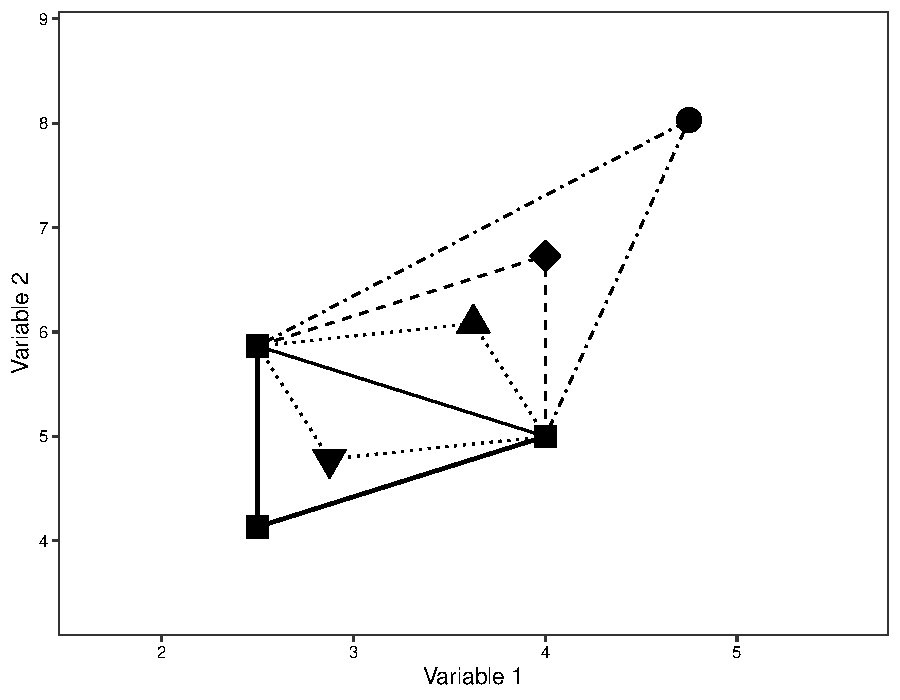
\includegraphics[width=0.6\textwidth]{chap2/images/simplexmov.pdf}
    \caption[Posibles movimientos de un símplex en un espacio bidimensional.]{Posibles movimientos de un símplex en un espacio bidimensional. Símplex original (\protect\squareblck), reflexión (\protect\squarerttdblck), expansión (\protect\circleblck), contracción del lado de la reflexión (\protect\triangleupblck) y contracción del lado del peor vértice (\protect\triangledownblck).}
    \label{fig:Simplexmov}
\end{figure}

Una de las ventajas más remarcables del algoritmo de optimización símplex es que el número de experimentos a realizar no crece de manera abrupta cuando se decide incluir más variables en el estudio. Por ejemplo, si en un diseño factorial a dos niveles se decide evaluar cuatro variables en lugar de tres, el número de experimentos de la matriz de diseño cambia de 8 a 16. Para la evaluación del simplex inicial, el número de experimentos cambia de cuatro a cinco. Esto hace menos importante el cribado de variables importantes que se recomienda antes del desarrollo de un diseño experimental más complejo.% (e.g.\ Matriz de Doehlert \citep{FERREIRA2004}).

El detalle de las reglas que gobiernan los algoritmos de optimización símplex y símplex modificado se describen con claridad en los capítulos tercero y cuarto del libro de \citet{simplexbook}. Ambos algoritmos han sido implementados en un paquete del lenguaje de programación \verb|R|. El paquete \verb|labsimplex| se encuentra disponible en de CRAN, y provee de herramientas para diseñar el símplex inicial, generar los vértices nuevos, visualizar gráficamente los movimientos del símplex y la evolución en la respuesta, entre otras cosas \citep{labsimplex}.


\section{Resumen}
En este capítulo se ha continuado con la exposición del litio como un elemento estratégico que es fundamental para la evolución de varias tecnologías que se proyectan a invadir el mundo, o que ya son ubicuas desde hace varios años. Se mencionaron aspectos relevantes de sus aplicaciones y de su contexto geopolítico. Se habló de las metodologías industriales que permiten su separación a partir de distintas fuentes naturales, y se hizo un resumen de algunas técnicas que se encuentran actualmente en desarrollo y que podrían ofrecer una alternativa para los procesos de extracción aplicados actualmente.

Las técnicas de separación cuyos conceptos son extrapolables a las \ac{PIM}s han sido descritas, y se han introducido los aspectos más importantes de la técnica aplicada en el presente trabajo. Se habló de las generalidades de las \ac{PIM}s y de los parámetros de transporte más importantes que caracterizan un sistema.

Finalmente se ha hablado de diseño de experimentos como la rama de la ciencia que está disponible para servir a todas las demás, haciendo más eficiente el trabajo en el laboratorio, y más robustas las conclusiones que pueden obtenerse a partir de los resultados disponibles.

\clearpage
\ChapBib{chap2/background}
    \chapter{Modelado Empírico de Perfiles de Transporte}\label{sec:NLS}
\section{Introducción}
Como se mencionó en la Sección \ref{sec:performanceparameters}, los perfiles de transporte otorgan una visión amplia del desempeño de un sistema de membranas para transportar una determinada especie. Los perfiles pueden analizarse rápidamente de manera gráfica, pero la principal desventaja de esta estrategia reside en que dos sistemas similares darán lugar a perfiles de transporte también similares, en cuyo caso, el análisis meramente gráfico no permitirá elucidar de manera objetiva las diferencias sutiles en el desempeño, a las que pueda haber lugar. Una alternativa sistemática de analizar los perfiles de transporte es a través de su modelamiento con ecuaciones empíricas. En este caso, se desea que los modelos escogidos describan apropiadamente los datos experimentales, y que los parámetros de las ecuaciones estén relacionados de alguna manera con los indicadores de desempeño del sistema. \index{Perfiles de transporte!Modelado de}


\citet{RODRIGUEZDESANMIGUEL2014} reportaron una ecuación que permite modelar los cambios de concentración de iones cromo en las disoluciones de alimentación y recuperación, en un proceso de transporte facilitado usando una PIM. Se encontró que los parámetros ajustables son de utilidad para optimizar los sistemas cuando son usados como variables respuesta en un diseño experimental (ver Sección \ref{sec:DoE}). Los parámetros se obtienen usando regresión no lineal por mínimos cuadrados (NLS)\acused{NLS}. En el reporte, las fracciones de ión cromo son ajustadas en función del tiempo $t$, con la siguiente ecuación:
\begin{equation}
    \Phi_i = A_ie^{-t/d_i} + y_{0,i}
\end{equation}
donde $\Phi_i$ son las fracciones de cromo en las disolucies de alimentación ($i = ali$) y recuperación ($i = rec$). $A_i$, $d_i$, y $y_{0,i}$ son los parámetros ajustables. $A_i$ se relaciona con el intercepto en el eje de las ordenadas del perfil de transporte, $d_i$ está relacionado con que tan marcado es el cambio en las fracciones en función del tiempo, y $y_{0,i}$ se relaciona con el valor límite que se alcanza en cada fase a largos tiempos de transporte.

Los parámetros ajustables en un mismo sistema difieren dependiendo de si se modela la fracción en la disolución de alimentación o en la de recuperación y esto impide que puedan ser promediados entre si. Para usar los parámetros los autores sugirieron dos funciones que denominaron $G_{feed}$ y $G_{strip}$. Estas funciones combinan los parámetros de regresión para cada disolución de una manera similar a como lo haría una función de deseabilidad.
\begin{equation}
    G_{feed}=\frac{1}{y_{0,ali}d_{ali}};\qquad G_{strip}=\frac{y_{0,rec}}{d_{rec}}
\end{equation}
La maximización de $G_{feed}$ y $G_{strip}$ por medio de un diseño experimental, permitió la obtención de las mejores condiciones para el proceso de transporte bajo estudio \citep{RODRIGUEZDESANMIGUEL2014}. Una propuesta similar de modelado empírico de procesos de transporte se utilizó en el presente trabajo, y su descripción se hace en la siguiente sección.

\section{Nueva propuesta}
%JCCA: ¿Por qué no buscar modelar la cinética de tranasporte, en lugar de utilizar un modelo empírico como este? Revisa, por ejemplo, Biophysical Chemistry, 35 (1990) 85-95 Kinetic model for membrane transport 1. Effects of membrane volume and partitioning kinetics.
%CAPC Holy damn shit! fuck! Admitamos inferioridad intelectual y tratemos de vender nuestra mierda mediocre :c
Modelar la cinética del proceso de transporte considerando la dinámica de todos los pasos involucrados permite estudiar de manera rigurosa el comportamiento del sistema, sin necesidad de recurrir a modelos empíricos y en algunos casos, haciendo un mínimo número de asunciones muy razonables. Estos modelos tienen la belleza de reflejar adecuadamente la realidad de los fenómenos bajo estudio \citep{MAKINO199085}. Sin embargo, el precio a pagar por cualidades tan apetecibles es con frecuencia una elevada complejidad matemática en el modelo, lo cual puede dificultar el avance de una investigación en la que se buscan las mejores condiciones para el transporte selectivo de una especie a través de una membrana. Acá es donde entran a jugar los modelos empíricos que por lo general son mucho más simples y requieren una cantidad mucho menor de información del sistema bajo estudio. Estos modelos empíricos son muy prácticos y pueden usarse en procesos de optimización, gracias a que la obtención de sus parámetros es con regularidad muy fácil y rápida. 

En el desarrollo del presente trabajo se observó que las fracciones de las especies en función del tiempo se comportan de manera similar a las cinéticas enzimáticas tipo Michaelis-Menten \citep{Johnson2011}, o a las isotermas de adsorción tipo Langmuir \citep{Atkins}. Esto sugiere que los perfiles de transporte pueden ser modelados con ecuaciones similares a las utilizadas en los fenómenos mencionados. Las ecuaciones a las que se ajustaron los perfiles de transporte para las disoluciones de alimentación y de recuperación, como fracción transportada en función del tiempo ($\Phi_{ali}(t)$ y $\Phi_{rec}(t)$, respectivamente) se muestran a continuación.

\begin{equation}\label{eq:NLSCRIS}
    \Phi_{ali}=1-\frac{\alpha_{ali} t^\kappa}{\beta_{ali}^{-1}+t^\kappa};\qquad\Phi_{rec}=\frac{\alpha_{rec} t^\kappa}{\beta_{rec}^{-1}+t^\kappa}
\end{equation}

donde $\alpha_i$ y $\beta_i$ se relacionan con los valores máximos transportados y la rapidez a la que ocurre dicho proceso, respectivamente. Valores altos de $\alpha$ y de $\beta$ implican procesos de transporte más eficientes y más veloces, respectivamente. $\kappa$ es igual a uno en la mayoría de los casos y es usado para mejorar el ajuste de las ecuaciones propuestas dado que algunos sistemas pueden mostrar algo de excentricidad que debe ser corregida en la ecuación empírica. Este parámetro $\kappa$ no es hallado por \ac{NLS} sino que debe definirse para cada conjunto de experimentos. Para que los valores de $\alpha$ y $\beta$ de dos sistemas puedan ser comparados entre sí, debe usarse el mismo valor de $\kappa$ en la regresión no lineal.


Para ilustrar la variación en los perfiles de transporte con los parámetros de la Ecuación \ref{eq:NLSCRIS} se simularon procesos de transporte variando dichos parámetros y los resultados se muestran en la Figura~\ref{fig:Modelssim}.

\begin{figure}[htbp]
    \centering
    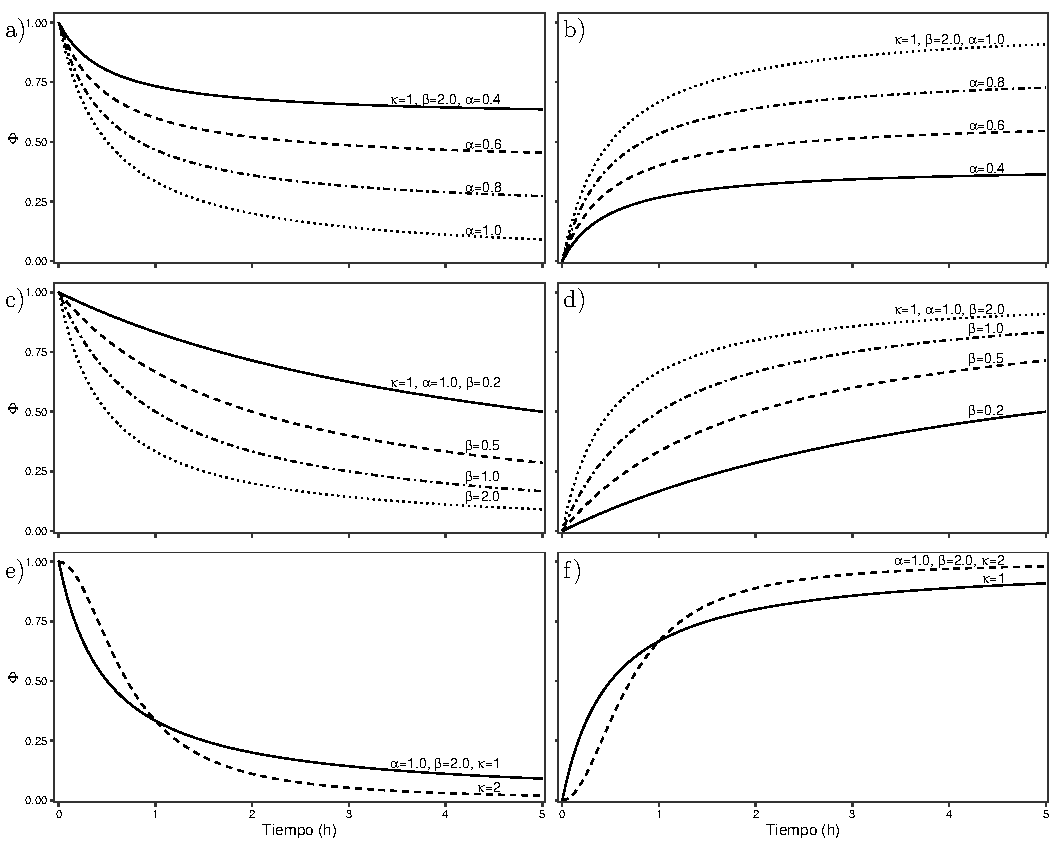
\includegraphics[width = \textwidth]{chap2/images/thesis-models.pdf}
    \caption[Perfiles de transporte simulados con la ecuación propuesta.]{Perfiles de transporte simulados con la ecuación propuesta usando distintos valores de $\alpha$, $\beta$ y $\kappa$ para las disoluciones de alimentación (a., c. y e.) y recuperación (b., d. y f.).}
    \label{fig:Modelssim}
\end{figure}

Puede observarse que para valores de $\beta$ y $\kappa$ constantes (Figuras \ref{fig:Modelssim}(a) y (b)), valores más altos del parámetro $\alpha$ se traducen en valores más pequeños y más grandes para la fracción remanente en la disolución de alimentación y la transportada hacia la disolución de recuperación, respectivamente, para tiempos en los que el sistema ha alcanzado un estado estacionario. 

Cuando los parámetros $\alpha$ y $\kappa$ se mantienen constantes (Figuras \ref{fig:Modelssim}(c) y (d)), los perfiles de transporte que tienden más rápido hacia el estado estacionario presentan valores de $\beta$ más grandes. Para el caso más frecuente en el que $\kappa=1$, el parámetro $\beta$ representa el tiempo al cual la fracción transportada es la mitad de la que será transportada  cuando el sistema alcance el estado estacionario.

Las Figuras \ref{fig:Modelssim}(e) y (f) muestran el cambio en los perfiles de transporte cuando los parámetros $\alpha$ y $\beta$ son constantes, y cambia el parámetro $\kappa$. El comportamiento de las curvas varía principalmente en los primeros momentos del experimento. A pesar de que los parámetros $\alpha$ y $\beta$ son iguales en ambos gráficos, un valor más grande de $\kappa$ produce curvas que llegan más rápido a su valor límite pero que parecen tener un pequeño tiempo de inducción en el que el proceso de transporte se ralentiza. Esto ha sido denominado excentricidad y se ha incluido en la Ecuación \ref{eq:NLSCRIS} para permitir que el modelo abarque un mayor número de sistemas, con un ajuste satisfactorio. Dicho parámetro debe definirse y no debe ser modificado para modelar perfiles de transporte experimentales que hayan sido obtenidos bajo condiciones relativamente similares.


Las ecuaciones que se proponen tienen algunas ventajas respecto a las propuestas en nuestro grupo de investigación hace unos años \citep{RODRIGUEZDESANMIGUEL2014}:
\begin{itemize}
    \item Si el sistema es bien comportado (i.e.\ no hay acumulación significativa de especies en la membrana) los valores de $\alpha$ y $\beta$ son prácticamente iguales para los datos de las disoluciones de alimentación y de recuperación.
    \item Los parámetros $\alpha$ y $\beta$ de cada disolución al ser equivalentes, pueden ser combinados entre sí usando promedios ponderados considerando su respectiva incertidumbre proveniente de la falta de ajuste del modelo \citep{borenstein2011}. Los parámetros obtenidos de esta manera pueden considerarse más robustos y su error asociado es menor.
    \item El número de parámetros que deben ser encontrados por \ac{NLS} es menor. Si el desempeño de dos modelos empíricos es prácticamente el mismo (esto puede ser juzgado por medio de las sumas de los residuales al cuadrado), usualmente se prefiere el más simple.
    \item No hay una combinación posible de parámetros en la que para un tiempo $t=0$, la fracción remanente en la disolución de alimentación sea diferente de uno o la fracción transportada hacia la fase de recuperación sea diferente de cero. Esto es consistente con lo que ocurre en el proceso de extracción.
\end{itemize}   



En el paquete de R \verb|transmem| (ver Capítulo \ref{sec:transmem66i}) se ha incorporado una función para obtener de manera sencilla los parámetros de regresión del modelo propuesto en este trabajo, y también del modelo propuesto por \citet{RODRIGUEZDESANMIGUEL2014}. La función se llama \verb|transTrend()| y su uso se explica en la Sección Anexa \ref{sec:transmemManual}.


\ChapBib{chap2b/chap2b}
    \chapter{Desarrollo Experimental}
\vspace{-1\baselineskip}El esquema de la Figura \ref{fig:expresumen} ilustra grosso modo el desarrollo experimental del trabajo de investigación. Este capítulo presenta los protocolos principales que se siguieron en los experimentos realizados. Algunas metodologías adicionales se incluyeron en las secciones anexas.\enlargethispage{3\baselineskip}
{\floatstyle{boxed}
\restylefloat{figure}
\begin{figure}[H]
    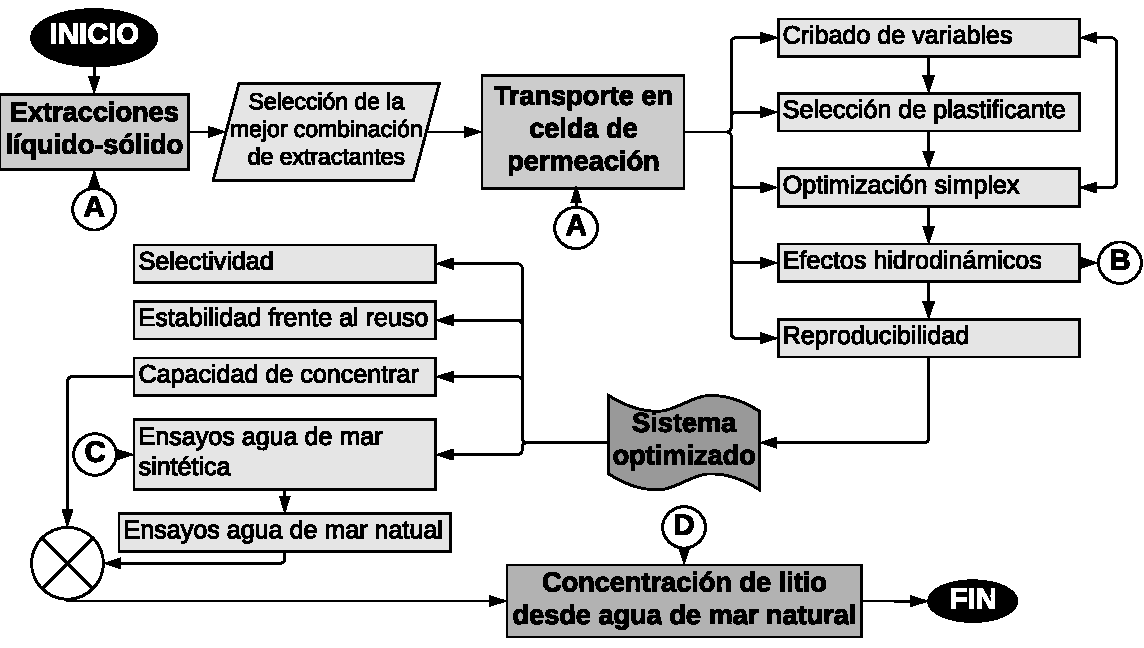
\includegraphics[width=\textwidth]{chap3/summary.pdf}
    \caption[Resumen esquematizado del desarrollo experimental.]{Resumen esquematizado del desarrollo experimental. (A): Determinación de cationes metálicos, (B): Medición de velocidad de giro de las propelas, (C): Precipitación de calcio y magnesio, (D): Microtitulación ácido-base.}
    \label{fig:expresumen}
\end{figure}}

\clearpage\section{Reactivos y disoluciones}
Todas las disoluciones acuosas fueron preparadas usando agua desionizada y reactivos grado analítico. Los proveedores de los extractantes y plastificantes utilizados para la preparación de las membranas se muestran en la Tabla \ref{tab:extractants}. El \ac{CTA} (Aldrich) empleado como polímero base tiene, según el proveedor, un contenido de grupos acetilo de 43.6\% en masa y una masa molecular (promedio en masa) entre 72000 y 74000~g~mol\mnn. 

\begin{table}[H]
    \centering\footnotesize
    \begin{tabular}{@{}p{0.05cm}p{3.5cm}p{5cm}@{}}\toprule
        &\textbf{Nombre}&\textbf{Proveedor}\\\midrule
        \multicolumn{2}{@{}l}{\textit{Extractantes}}\\[-0.6ex]
         & LIX-54-100 (246.0)& Cognis Corporation\\
         & D2EHPA (322.4)& Sigma Aldrich\\
         & TEHP (434.6)& Sigma Aldrich\\
         & Cyanex~923 (348.0) & Cytec Canada Inc.\\
         & TBP (266.3)  & Sigma Aldrich\\
        \multicolumn{2}{@{}l}{\textit{Plastificantes}}\\[-0.6ex]
         & NPOE & Sigma Aldrich\\
         & T2EHP & Sigma Aldrich\\
         & TBEP  & Fluka\\\bottomrule
    \end{tabular}
    \caption[Extractantes y plastificantes empleados.]{Extractantes y plastificantes empleados. En paréntesis se indica la masa molecular de cada extractante en g~mol\mnn.}
    \label{tab:extractants}
\end{table}


Los reactivos diclorometano (\acs{DCM}) \acused{DCM} (J.T. Baker), cloruro de sodio (Químicos Monterey), cloruro de potasio (Merck), cloruro de calcio dihidratado (Merck), sulfato de magnesio heptahidratado (Merck), ácido clorhídrico (Sigma-Aldrich), hidróxido de amonio (Sigma-Aldrich), fosfato monohidrógeno de amonio (Merk) e hidróxido de sodio (Mallinckrodt) se usaron tal y como fueron recibidos. Disoluciones de cloruro de litio y cloruro de magnesio fueron preparadas di\-sol\-vien\-do sus respectivos carbonatos (Aldrich) en un ligero exceso de ácido clorhídrico.

Todas las disoluciones y sus subsecuentes diluciones fueron preparadas gravimétricamente en una balanza analítica OHAUS Adventurer AX224. Esta práctica concede una gran versatilidad para hacer las disoluciones y permite el manejo de cantidades de disolución muy pequeñas, sin sacrificar precisión en la toma de la alícuota. Adicionalmente, preparar las disoluciones en masa permite un uso más eficiente del material de laboratorio y del tiempo del experimentador.

Cuando se indica que un reactivo se usó {seco}, se hace alusión a que la posible humedad presente en dicho reactivo fue retirada usando un horno de convección forzada a una temperatura de 80$^o$C durante una hora y el reactivo se dejó enfriar en un desecador donde permaneció hasta el momento de su uso.

La cuantificación de cationes metálicos se hizó por espectrometría de absorción atómica por llama (\acs{FAAS})\acused{FAAS} y espectrometría de emisión atómica por llama (\acs{FAES})\acused{FAES}, en un espectrómetro de absorción atómica Perkin-Elmer 3100, usando las configuraciones recomendadas por el fabricante \citep{perkin}. Los detalles del sistema analítico se describen en el Anexo \ref{sec:quantification}.

El protocolo de lavado del material de laboratorio implicó tres etapas principales:
\begin{enumerate}
    \item Lixiviación de especies metálicas por inmersión en ácido nítrico al 10\% en volumen durante al menos 12 horas.
    \item Enjuague vigoroso con agua desionizada al menos tres veces.
    \item Secado en horno de convección forzada a una temperatura entre 60 y 80$^o$C y enfriamiento a temperatura ambiente.
\end{enumerate}


\subsection{Agua de mar sintética}\index{Agua de mar!sintética}
El agua de mar sintética fue preparada acorde a una receta simplificada de agua de mar que se usa en la determinación de constantes termodinámicas en agua de mar \citep{Sun2019}. La composición se muestra en la Tabla \ref{tab:seasintetic} \citep{Dickson1994}. En esta receta se consideran únicamente las especies cuya concentración es relativamente alta. Se incluyen los aniones cloruro y sulfato mientras los aniones bromuro y fluoruro son reemplazados por cloruro y los demás aniones son ignorados. El catión estroncio es reemplazado por calcio, el cual es considerado en conjunto con sodio, potasio y magnesio. El ion litio no se incluye en la receta simplificada pero se añadió a la concentración promedio reportada para agua de mar: 0.18~mg~kg\mnn\ (2.6\e{-5}~mol~kg\mnn) \citep{Evans2013}. 

La fuerza iónica de la disolución sintética es la misma que la fuerza iónica promedio reportada para el agua de mar real (0.697~mol~kg\mnn).

\begin{table}[H]
    \centering\footnotesize
    \begin{tabular}{@{}p{0.05cm}lld{2.3}c@{}}\toprule
        &\multirow{2}{*}{\textbf{Especie}} & \multicolumn{2}{c}{\textbf{Concentración}}&\textbf{Rel. molar}\\
        &&mol~kg\mnn&\multicolumn{1}{c}{g~kg\mnn}&\multicolumn{1}{c}{\ce{M^n+}:\ce{Li^+}}\\\midrule
        \multicolumn{2}{l}{\textit{Aniones}}\\[-0.6ex]
        &\ce{Cl^-}  &0.549 &19.472&-\\
        &\ce{SO4^2-}&0.028 &2.720 &-\\
        \multicolumn{2}{l}{\textit{Cationes}}\\
        &\ce{Na^+}  &0.469 &10.785&18000\\
        &\ce{Mg^2+} &0.052 &1.284 &2030\\
        &\ce{Ca^2+} &0.010 &0.415 &400\\
        &\ce{K^+}   &0.010 &0.399 &390\\
        &\ce{Li^+}  &2.6\e{-5}&\multicolumn{1}{c}{1.8\e{-4}}&1\\\bottomrule
    \end{tabular}
    \caption{Composición del agua de mar sintética simplificada.}
    \label{tab:seasintetic}
\end{table}

\subsection{Muestras de agua de mar natural}\index{Agua de mar!natural}
Dos muestras de agua de mar natural fueron recolectadas manualmente en cercanías a las playas de Santa Marta-Colombia y de St. George Island-Estados Unidos (Figura \ref{fig:SWNmap}). En cada punto se recolectó cerca de un litro de agua de mar en botellas de poli(tereftalato de etileno) (PET)\acused{PET}, y las muestras fueron mantenidas bajo refrigeración hasta su uso. Previo a su uso, las muestras se filtraron por gravedad para remover arena y otros sólidos. Los puntos de recolección de las muestras fueron escogidos por la disponibilidad de las personas que se encargaron de hacer el muestreo.

\begin{figure}[htbp]
    \centering
    \subbottom{\begin{picture}(500,300)
               \put(0, 0){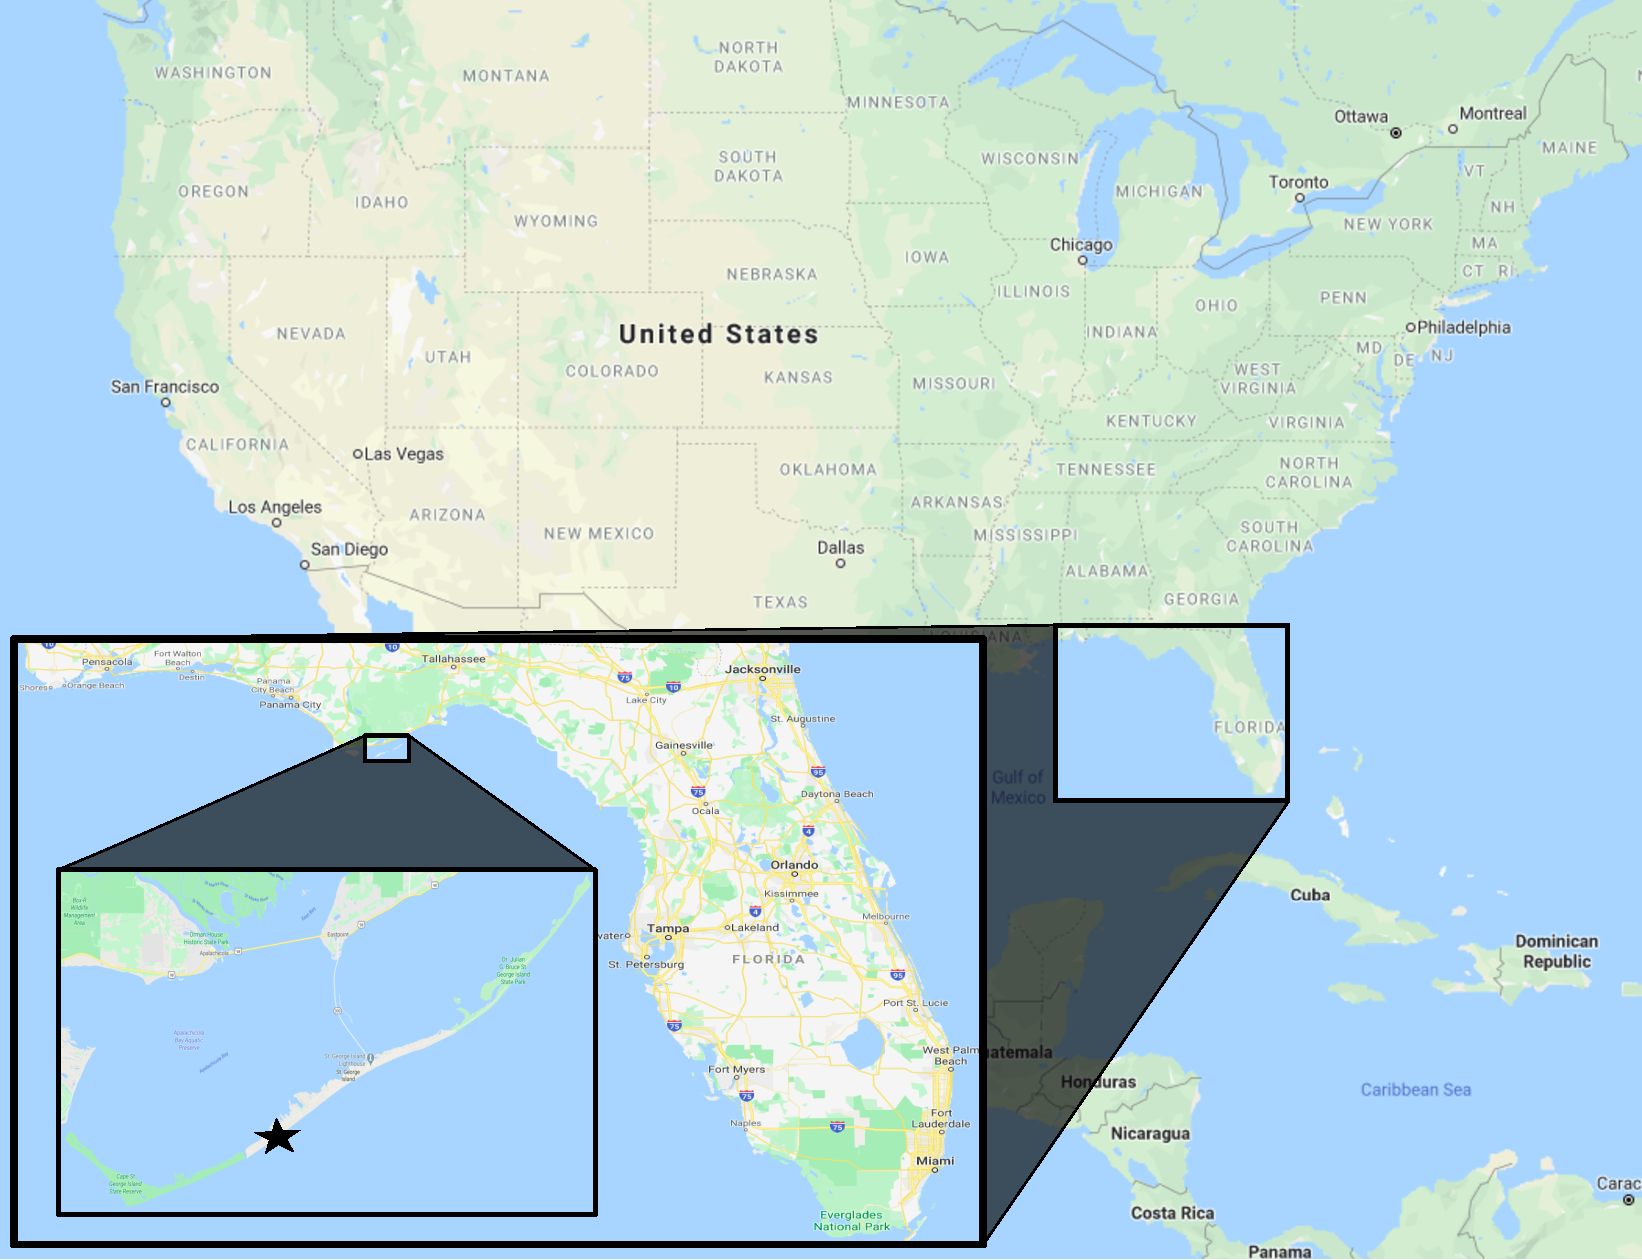
\includegraphics[width=\textwidth,trim={0 0 0 4cm}, clip]{chap3/SWN.pdf}}
               \put(3, 278){\Large a)}
               \end{picture}}\\%
    \subbottom{\begin{picture}(550,300)
               \put(0, 0){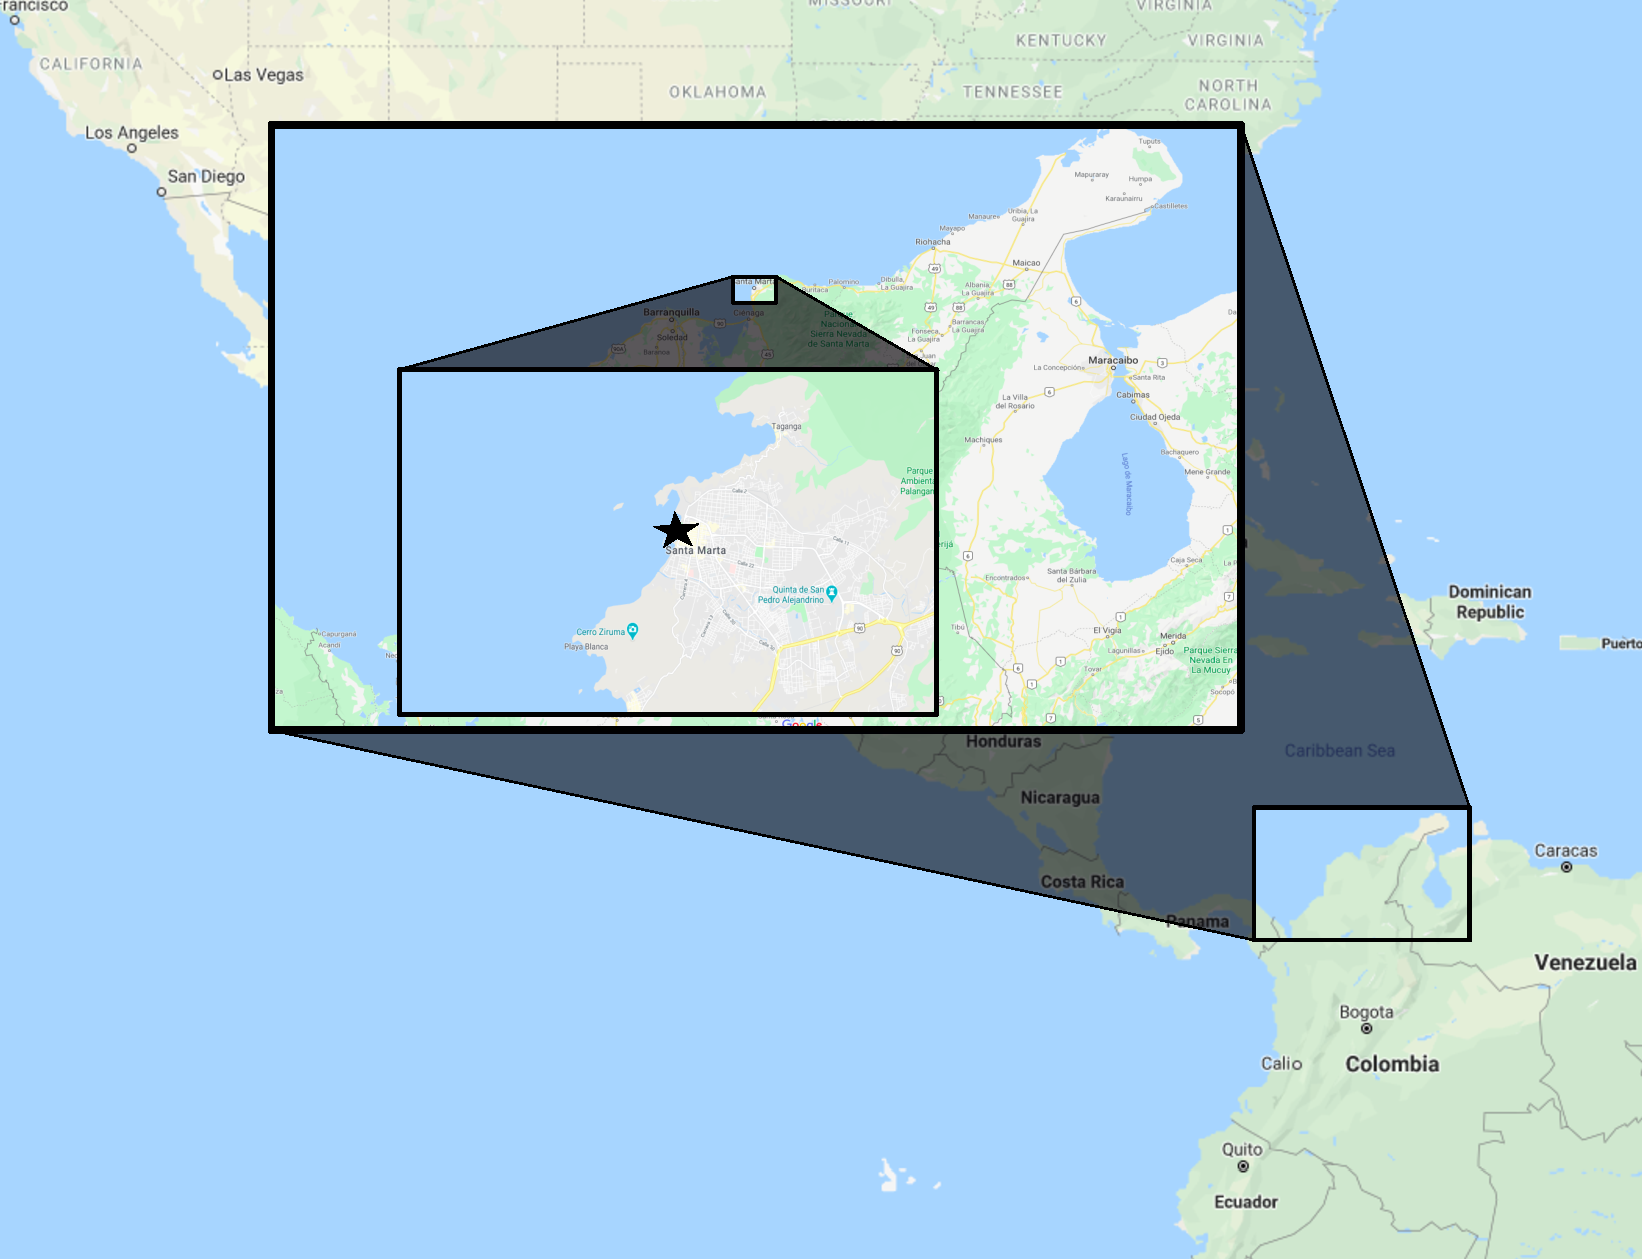
\includegraphics[width=\textwidth,trim={0cm 2.5cm 0cm 1.5cm}, clip]{chap3/SWS.pdf}}
               \put(3, 278){\Large b)}
               \end{picture}}
    \caption[Ubicación geográfica de los puntos de muestreo de agua de mar.]{Ubicación en  Estados Unidos (a) y en Colombia (b) de los puntos de muestreo (\protect\starfvpointsblck) de agua de mar natural.}
    \label{fig:SWNmap}
\end{figure}

\section{Elaboración de membranas poliméricas de inclusión}\index{PIM!elaboración}
Las membranas fueron preparadas por el método de vertido en molde descrito por varios autores \citep{Salazar-alvarez2005}. En un vaso de precipitados de 10~mL se toman cuidadosamente las masas escogidas de polímero base (\ac{CTA}), extractantes, y plastificante (la mayoría de las membranas no necesitaron plastificante en su formulación). Se añaden 10~mL de \ac{DCM} y la mezcla se agita magnéticamente durante aproximadamente dos horas hasta que se observa la disolución completa del polímero base. La disolución homogénea se transfiere cuantitativamente a la sección inferior de una caja Petri de vidrio (Pyrex\textregistered) y se cubre con su tapa respectiva. El disolvente se deja evaporar lentamente durante toda la noche en una campana de extracción sin encender. Se forman películas homogéneas que por lo general son flexibles y poseen buenas propiedades mecánicas. Las membranas pueden dejarse en las cajas de Petri por un periodo largo de tiempo sin que sufran un deterioro importante en su desempeño. 

Para retirar las membranas al momento de su uso se inunda la caja de Petri con agua desionizada y se corta el borde de la membrana que colinda con la pared circular del recipiente, usando la punta redonda de una microespátula delgada de acero inoxidable. Con estos dos pasos la membrana puede despegarse con facilidad, y el riesgo de que se dañe en este proceso disminuye considerablemente.

El grosor de las membranas se determinó usando un micrómetro digital de tornillo (Fowler IP54). La medición de grosor conlleva un deterioro a la membrana que impide su uso posterior para experimentos de transporte por lo que estas membranas ya no pueden usarse para nada más. Para medir el grosor, se dibuja una cuadrícula sobre la membrana usando un rotulador permanente de punta fina y se determina el grosor en cada cuadrado que tiene aproximadamente 0.5~cm de lado. Los valores que corresponden al centro con 1.25~cm a la redonda (región que está en contacto con las disoluciones) son promediados y el promedio es el valor que se reporta.

\section{Extracción líquido-sólido}\label{sec:liqsolex}\index{Extracción!líquido-sólido}
Las extracciones líquido-sólido se hicieron para seleccionar la combinación de extractantes con los que se trabajaría durante todo el proyecto. Se usó un agitador mecánico Burrell Scientific Wrist Action$^{TM}$ Modelo 75 cargado con tubos cónicos de 50~mL con tapa rosca (tubos de centrífuga). Para la extracción, se dispuso en el tubo una masa conocida de una disolución alcalina con ion litio (fase donadora) y una \ac{PIM}. Para maximizar el área de contacto de la disolución con la membrana, se procuró que ésta quedara suspendida en la disolución y no en contacto con la pared interior del tubo. La mezcla se agitó vigorosamente durante tres horas, al cabo de las cuales la membrana se extrajo con pinzas y se lavó cuidadosamente con agua desionizada. Posteriormente, la recuperación del ion litio extraído por la membrana se hizo con un protocolo similar usando una disolución de ácido clorhídrico (fase receptora). La concentración de ion litio en la fase donadora y receptora se determinó antes y después de cada proceso de agitación.

\section{Transporte en celda de permeación}
Los experimentos de transporte se hicieron en una celda de permeación (o celda de transporte) similar a la ilustrada en la Figura \ref{fig:celda}. La celda consta de dos compartimientos separables (semiceldas) que se encuentran conectados a través de un orificio circular de 2.5~cm de diámetro. En cada semicelda se disponen las disoluciones de alimentación y de recuperación, respectivamente. El orificio circular sirve para posicionar la membrana que queda firmemente sujetada entre las semiceldas que se mantienen juntas con firmeza, gracias al uso de pinzas clip metálicas para papel de 5~cm. El sello entre los compartimientos se logra con un empaque circular tipo \textit{o-ring}.

\begin{figure}[H]
    \centering
    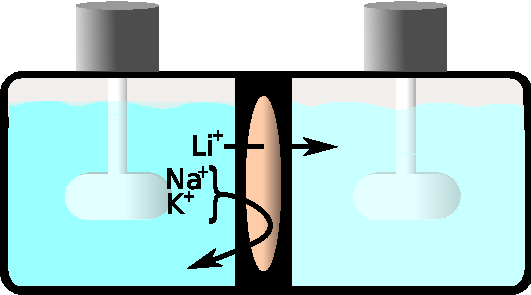
\includegraphics[width=0.5\textwidth]{chap3/PermCell}
    \caption{Celda de permeación usada en los experimentos de transporte.}
    \label{fig:celda}
\end{figure}

Las semiceldas son agitadas mecánicamente con propelas de doble aspa de teflón, impulsadas por motores eléctricos controlados individualmente por moduladores de amplitud de pulso (\acs{PWM})\acused{PWM}. Por lo general se inicia con 85~g de disolución en cada compartimiento y periódicamente se toman pequeñas alícuotas (entre 800 y 1500~$\mu$L) de ambas disoluciones. Las alícuotas son almacenadas en viales Eppendorf\textregistered~ para cuantificar posteriormente las especies de interés (Anexo \ref{sec:quantification}).

Las condiciones del proceso de transporte (composición de las membranas y de las disoluciones de alimentación y recuperación) fueron optimizadas por medio de diseños experimentales factoriales fraccionados y del algoritmo simplex modificado. Para esto se usaron los paquetes de R \verb|FrF2| de \cite{FrF2} y \verb|labsimplex| de \cite{labsimplex}. Los detalles de las matrices de diseño o de la configuración inicial del simplex se incluyen en la sección de resultados.

\subsection{Efecto de las condiciones hidrodinámicas y reproducibilidad}\label{sec:hydroexpe}
Las condiciones hidrodinámicas fueron evaluadas con experimentos de transporte modificando la rapidez de rotación de la propela ($\Theta$) que agita cada disolución. Esta rapidez de rotación se determinó siguiendo el protocolo descrito en el Anexo \ref{App:tracker}. Inicialmente se evaluaron valores de $\Theta$ entre 360 y 920 revoluciones por minuto (\ac{RPM}\acused{RPM}) mientras la rapidez de agitación en la fase de recuperación se mantuvo constante en $960\pm60$~\ac{RPM}. Cada proceso de transporte fue monitoreado durante 5 horas y se usaron disoluciones de alimentación de ion litio en ausencia de interferentes.

Posteriormente, para evaluar la repoducibilidad del proceso, el transporte se llevó a cabo en días distintos, en un intervalo de valores de rapidez de agitación más pequeño (510 a 665 \ac{RPM}). Se usó como variable de bloqueo la celda en la que se llevó a cabo el transporte (Celda A y Celda B) y se usaron disoluciones de alimentación con ion litio en presencia de un exceso molar 1:20 de iones sodio. La concentración de ambas especies fue monitoreada durante cinco horas.

\subsection{Selectividad frente a sodio, potasio y magnesio}\index{PIM!selectividad}
La selectividad del sistema optimizado frente a los iones sodio, potasio y magnesio (cationes interferentes) se estudió por medio de transportes usando disoluciones de alimentación con ion litio 2~mg~kg\mnn\ en presencia de cada uno de los cationes interferentes en relaciones molares \ce{Li+}/\ce{M^n+} de 1:1, 1:10 y 1:100. Se usó una disolución de alimentación con concentración inicial de hidróxi\-do de amonio de 0.016~mol~kg\mnn\ y una disolución de recuperación de ácido clorhídrico a una concentración inicial de 0.10~mol~kg\mnn. Cada proceso de transporte fue monitoreado durante 5 horas.

\subsection{Capacidad de reuso de la membrana}\label{sec:reuseex}\index{PIM!estabilidad}
La capacidad de reuso de la membrana se estudió repitiendo el proceso de transporte renovando las disoluciones de alimentación y de recuperación. El ciclo se llevó a cabo 10 veces consecutivas usando la misma membrana optimizada y una disolución de alimentación ideal (hidróxido de amonio 0.016~mol~kg\mnn\ y ion litio 2~mg~kg\mnn) en la que el ion litio era el único catión metálico presente (proveniente de cloruro de litio). Se usó ácido clorhídrico 0.10~mol~kg\mnn\ como disolución de recuperación.

\subsection{Concentración de ion litio}\label{ss:concentracion}
Los experimentos de concentración fueron similares a los descritos en la Sección \ref{sec:reuseex}, con la diferencia de que la disolución de recuperación no se renovó entre ciclos con el fin de concentrar el ion litio en esta fase. Adicionalmente el número de ciclos consecutivos fue menor. En primera instancia, se utilizo la misma disolución de alimentación ideal de la sección anterior y esta fue renovada cuatro veces (cinco ciclos). Posteriormente, luego de comprobar que el sistema era capaz de extraer ion litio de agua de mar sintética y natural (Sección \ref{sec:resultsSSS}), se usó agua de mar natural a partir de la cual se extrajo el ion litio durante cuatro ciclos. 

Para concentrar ion litio desde agua de mar fue necesario restaurar la concentración de iones hidronio en la disolución de alimentación al final de cada ciclo usando ácido clorhídrico 1~mol~kg\mnn. No se mantuvo constante la acidez de la disolución de recuperación porque se quiso evitar el uso de sustancias amortiguadoras de pH que representarían variables adicionales que considerar al momento de optimizar el sistema. La cantidad de ácido necesaria para ajustar nuevamente la concentración de iones hidronio al valor deseado fue estimada considerando la concentración de ácido remanente, la cual fue determinada por microtitulación con hidróxido de sodio (Anexo \ref{Sec:microfuck}).

\subsection{Extracción de ion litio de agua de mar}\index{Agua de mar}
Para extraer ion litio de agua de mar fue necesario separar del medio los cationes divalentes calcio y magnesio antes del proceso de transporte (Sección \ref{sec:selecresults}). La manera más sencilla y eficiente de hacerlo es por precipitación como se describe en el siguiente apartado. Como resultado de una de las etapas de precipitación, la disolución de alimentación queda con un exceso de iones hidroxilo que provee a la disolución de un medio lo suficientemente alcalino como para favorecer el transporte de iones litio hacia la fase de recuperación. Debido a esto, no fue necesaria la adición de hidróxido de amonio para el proceso de transporte.

%En los ensayos con agua de mar natural, la concentración en exceso de iones hidroxilo fue determinada por microtitulación ácido-base y se estudió el efecto de su valor inicial en el transporte de litio a través de la membrana. Para esto, distintas proporciones de los iones hidroxilos en exceso fueron neutralizados con ácido clorhídrico 1~mol~kg\mnn\ a concentraciones iniciales de hidróxido de 0.04, 0.03, 0.02, 0.01 y 0.00~mol~kg\mnn.
 
\subsubsection{Eliminación de cationes divalentes calcio y magnesio}\label{sec:preci}
Los iones calcio y magnesio fueron eliminados de las matrices de agua de mar sintética y agua de mar natural por precipitación en dos pasos. En primera instancia, el magnesio es removido como hidróxido usando hidróxido de sodio a una concentración de 0.15 mol~kg\mnn. Esto aumenta apreciablemente la cantidad de iones sodio presente en la muestra. Una porción de los iones calcio coprecipitan con el magnesio como hidróxido. En un segundo paso, los iones calcio remanentes son removidos como fosfatos al añadir fosfato monohidrógeno de amonio a una concentración 0.005~mol~kg\mnn. 

Tras la adición de cada reactivo precipitante, la mezcla es agitada vigorosamente por cinco mi\-nu\-tos y posteriormente se separan las fases por centrifugación a 3000 \ac{RPM} durante cinco minutos (IEC HN-SII Centrifuge, Damon/IEC Division).

\clearpage\ChapBib{chap3/experimental}
    \chapter{Paquete \trm}\label{sec:transmem66i}

\section{Introducción}
El tratamiento de datos para la obtención de resultados numéricos y gráficos es un paso muy importante en el estudio de todos los sistemas. Los procesos de transporte estudiados en el presente trabajo no generan una gran cantidad de datos y su tratamiento no es particularmente complicado. En muchos lugares, estas tareas se cumplen usando herramientas como hojas de calculo que realmente no fueron diseñadas para su aplicación en ciencias exactas. El uso de programas como Microsoft Excel\textregistered\ la mayoría de las veces no acarrea consecuencias negativas en los resultados obtenidos, pero muchos de los procedimientos deben ser llevados a cabo siguiendo protocolos tediosos que involucran mucho trabajo {manual} que disminuye sus capacidades de reusabilidad y adaptabilidad \citep{Incerti2019}. Los gráficos generados por defecto en este tipo de plataformas distan de los conceptos de la gramática de los gráficos \citep{Wilkinson2005} y mucho esfuerzo adicional se requiere para producir gráficos apropiados. 

Existen múltiples alternativas más apropiadas que se encuentran basadas en lenguajes de programación modernos que ganan cada vez más popularidad. Entre las muchas ventajas que presentan estos lenguajes, está que la mayoría de las veces son de código abierto y eso asegura su disponibilidad para todas las personas, sin importar el presupuesto que tengan asignado para su investigación. Su uso involucra un gasto computacional mucho menor, por lo que análisis muy poderosos pueden hacerse en tiempos cortos empleando computadoras muy convencionales. Estas alternativas son altamente potencializables por medio de librerías o {paquetes} que son un conjunto de funciones pensadas para resolver una serie de problemas particulares. Un gran número de paquetes se encuentran disponibles y los números van en aumento. Los lenguajes de programación de código abierto exitosos generan una gran comunidad de usuarios y desarrolladores, dispuestos a brindarse ayuda mutua a través de diversas plataformas como \url{https://stackoverflow.com/}.


\R\ es un entorno de programación que permite computación estadística y representación gráfica de datos \citep{R}. Una excelente introducción a \R\ fue escrita por \citet{Venables2004}. \R\ se encuentra disponible para la mayoría de los sistemas operativos comunes y está constantemente bajo actualización y mejora. El repositorio oficial \ac{CRAN} contiene más de 15000 librerías plenamente documentadas y disponibles para cualquier persona con acceso a internet. Existen numerosos paquetes de gran utilidad para distintas ramas de la química. Algunos ejemplos importantes se muestran en la Tabla \ref{tab:Rpackages}.

\begin{table}[H]
    \centering\footnotesize
    \begin{tabular}{@{}lp{9.55cm}l@{}}\toprule
        \textbf{Nombre} & \textbf{Propósito} & \textbf{Referencia} \\\midrule
         \verb|chemometrics|&Análisis estadístico multivariado en quimiometría &\citet{Filzmoser2017}\\
         \verb|propagate|&Propagación de incertidumbre &\citet{Spiess2018}\\
         \verb|FrF2|&Creación y análisis de diseños factoriales fraccionados de dos niveles &\citet{FrF2}\\
         \verb|rsm|&Métodos de análisis de respuesta& \cite{Lenth2009}\\
         \verb|DoE.base|&Diseños factoriales fraccionados &\citet{Gromping2018}\\
         \verb|eChem|&Simulación de experimentos de electroquímica &\citet{Harvey2015}\\
         \verb|spectral|&Métodos comunes en el análisis de datos espectrales &\citet{SeilMayer2019}\\
         \verb|ChemoSpec|&Quimiometría exploratoria para espectroscopía &\citet{Hanson2020}\\
         \verb|AFM|&Análisis de imágenes de microscopía de fuerza atómica &\citet{Beauvais2019}\\
         \verb|SixSigma|&Herramientas \textit{seis sigma} para control de calidad y mejora continua &\citet{Cano2015}\\
         \verb|RGCxGC|&Análisis de datos bidimensionales de cromatografía de gases&\cite{Quiroz2020}\\
         \verb|labsimplex|&Algorítmos de optimización simplex para aplicaciones de laboratorio&\citet{labsimplex}\\\bottomrule
    \end{tabular}
    \caption{Ejemplos de paquetes de R diseñados para distintas áreas de la química.}
    \label{tab:Rpackages}
\end{table}

Se escribieron y documentaron distintas funciones en \R\ para automatizar el tratamiento de los numerosos conjuntos de datos generados durante el presente trabajo de investigación. Estas funciones fueron posteriormente aglomeradas en el paquete \trm. En el paquete se incluyeron algunos conjuntos de datos que fueron producidos durante algunos de los experimentos realizados para ilustrar el uso de las funciones. El manual oficial del paquete se encuentra en el Anexo \ref{sec:transmemManual}. El código fuente del paquete puede encontrarse en el repositorio \url{https://github.com/Crparedes/transmem}. A pesar del gran número de librerías disponibles en \ac{CRAN}, hasta donde sabemos, no existe aún ninguna librería disponible para el tratamiento de datos provenientes de procesos de transporte a través de membranas.

En este capítulo se esquematiza el uso general del paquete y se describe su proceso de instalación. Los detalles de las funciones pueden ser encontradas en el manual oficial donde se encuentran ejemplos prácticos que hacen uso de los conjuntos de datos mencionados.

%La información que se alimenta a las funciones de \trm en la mayoría de los casos puede ser cargada desde un archivo de texto plano o ingresada manualmente dependiendo de las características de los instrumentos empleados. En el presente capítulo se ha optado por el segundo enfoque el cual, a pesar de sus limitaciones prácticas, ofrece un panorama más claro y reproducible para quien desee aprender a usar el paquete desde ceros. Para más detalles sobre cómo cargar datos desde archivos vea el Capítulo 7 del libro de \cite{Venebles2004}.
\clearpage
\section{Instalación del paquete}
\enlargethispage{1\baselineskip}
Antes de instalar \trm\ es necesario tener instalado \R\ en una versión igual o superior a la 3.5.0. Se recomienda adicionalmente la instalación de Rstudio (\url{https://rstudio.com/}) que es una \ac{GIU} diseñada para facilitar grandemente el trabajo de datos con \R. 

El paquete ha sido aceptado en el repositorio oficial \ac{CRAN}. La ultima versión oficial puede instalarse con el comando general:
\begin{lstlisting}[belowskip=-2.6\baselineskip]
install.packages('transmem')
\end{lstlisting}

La última versión construida del paquete\footnote{El paquete recibe actualizaciones regularmente.} \trm\ puede descargarse directamente desde su repositorio en Github uśando el paquete \verb|devtools| \citep{Hadley2019}:
\begin{lstlisting}[belowskip=-2.6\baselineskip]
if (!require("devtools")) install.packages("devtools")
devtools::install_github("Crparedes/transmem")
\end{lstlisting}


Si el paquete ha sido instalado correctamente aparecerá en la pantalla de comandos de \R:
\begin{lstlisting}
#    > Installing package into '/home/cris/R/x86_64-pc-linux-gnu-library/3.6'
#    >   (as 'lib' is unspecified)
#    > * installing *source* package 'transmem' ...
#    > ** using staged installation
#    > ** R
#    > ** data
#    > *** moving datasets to lazyload DB
#    > ** byte-compile and prepare package for lazy loading
#    > ** help
#    > *** installing help indices
#    > ** building package indices
#    > ** testing if installed package can be loaded from temporary location
#    > ** testing if installed package can be loaded from final location
#    > ** testing if installed package keeps a record of temporary installation path
#    > * DONE (transmem)
\end{lstlisting}
El paquete estará listo para ser cargado en el ambiente de trabajo para poder usar sus funciones:

\begin{lstlisting}[belowskip=-2.6\baselineskip]
library('transmem')
\end{lstlisting}

\clearpage
\section{Operación del paquete}
La Figura \ref{fig:chap4esquema} contiene el esquema de las funciones principales del paquete. En el mapa conceptual se sugiere una secuencia inicial de tres pasos pensada para transformar los datos experimentales al formato apropiado para las funciones del paquete. La matriz de datos del transporte contiene la concentración o la fracción de una especie en función del tiempo en ambas disoluciones (alimentación y recuperación). Esta matriz (que es en realidad un \textit{data.frame}) es la que se usa para producir los resultados numéricos y generar las representaciones gráficas pertinentes.

{\floatstyle{boxed}
\restylefloat{figure}
\begin{figure}[H]
    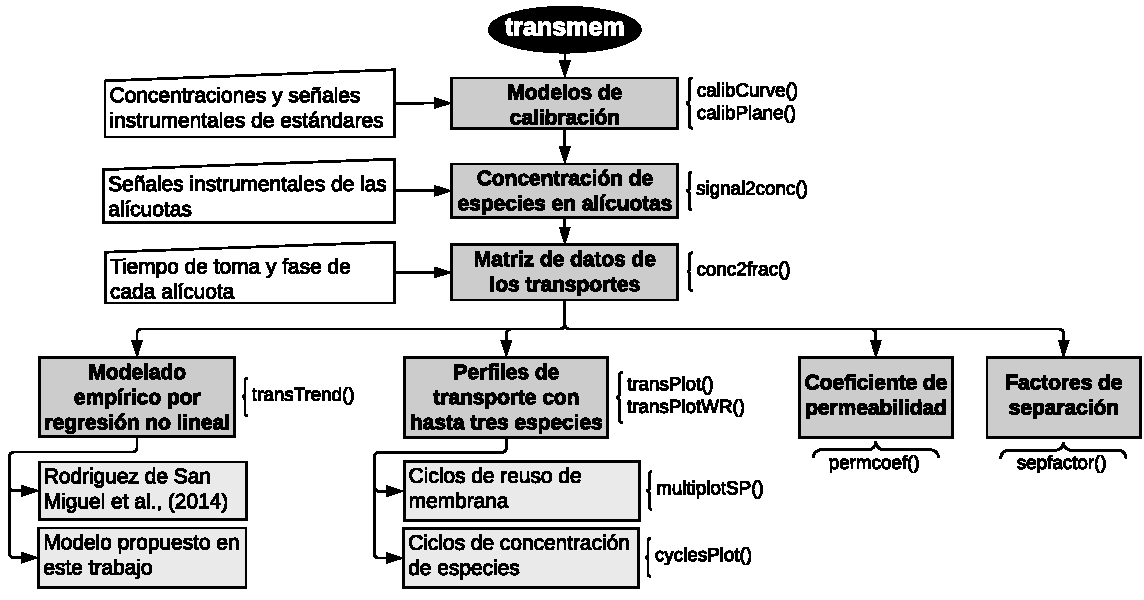
\includegraphics[width=\textwidth]{chap4/Chapter4Thesis.pdf}
    \caption{Esquema de las funciones principales del paquete \trm.}
    \label{fig:chap4esquema}
\end{figure}
}

Para conocer como se usa alguna función se recomienda ver el manual de referencia del paquete en el Anexo \ref{sec:transmemManual}. Una alternativa es usando la función \verb|help()| luego de haber cargado el paquete. Para ver la ayuda de una función en particular, escriba en la ventana de comandos de \R: 
\begin{lstlisting}
help("nombre_de_la_funci\'on")
\end{lstlisting}

La interfaz gráfica de la aplicación web se encuentra en desarrollo y se está buscando un servidor oficial en la Facultad para ponerlo a disposición de la comunidad. Mientras el espacio en el servidor es asignado, la aplicación puede ser utilizada (con algunas limitantes) en la página \url{https://crparedes.shinyapps.io/transmem_shinyapp/}.
\clearpage
\ChapBib{chap4/Chap4}
%\section{Creación de modelos de calibración}
%Monitorear la concentración de una especie en función del tiempo es fundamental en muchos procesos de transporte a través de membranas. Esto por lo general involucra la comparación de las señales que producen las muestras en respuesta a un estímulo para compararlas con las producidas por disoluciones estándar de concentración conocida. La comparación se hace por métodos de regresión que involucran curvas de calibración y eventualmente, planos de calibración, entre otros. Para crear una curva de calibración debe conocerse la concentración de la especie de interés y la señal producida por la misma para cada estándar. 

%\begin{lstlisting}[belowskip=-2.6\baselineskip]
%curvelithium <- data.frame(conc   = c(0.00, 0.05, 0.23, 0.73, 0.92, 1.30, 1.66, 2.11),
%                           signal = c(0.000, 0.036, 0.162, 0.477, 0.586, 0.797, 0.971, 1.169))
%lithiummodel <- calibCurve(curvelithium, order = 2)
%\end{lstlisting} 

%Se genera un gráfico con la información de la curva de calibración. El gráfico se muestra en la Figura \ref{fig:calcurvetrm1}(a). El comando \verb|plot(lithiummodel$residuals)| hace el gráfico de residuales de la regresión para evaluar la pertinencia del modelo escogido, este gráfico se muestra en la Figura \ref{fig:calcurvetrm1}(b). Para visualizar en detalle el modelo generado, la significancia estadística de cada parámetro y la significancia estadística de toda la regresión se usa la función \verb|summary()|. 
%\begin{lstlisting}[belowskip=-2.6\baselineskip]
%summary(lithiummodel)
%#      > Call:
%#      > lm(formula = Signal ~ Conc + I(Conc^2), data = curveN)
%#      > 
%#      > Residuals:
%#      >          1          2          3          4          5          6          7... 
%#      > -0.0014330 -0.0003988  0.0026637  0.0003075 -0.0019808  0.0018193 -0.0015631...
%#      > 
%#      > Coefficients:
%#      >              Estimate Std. Error t value Pr(>|t|)    
%#      > (Intercept)  0.001433   0.001293   1.108    0.318    
%#      > Conc         0.702864   0.003280 214.264 4.20e-11 ***
%#      > I(Conc^2)   -0.070992   0.001589 -44.674 1.06e-07 ***
%#      > ---
%#      > Signif. codes:  0 '***' 0.001 '**' 0.01 '*' 0.05 '.' 0.1 ' ' 1
%#      > 
%#      > Residual standard error: 0.001971 on 5 degrees of freedom
%#      > Multiple R-squared:      1,	Adjusted R-squared:      1 
%#      > F-statistic: 1.725e+05 on 2 and 5 DF,  p-value: 7.995e-13
%\end{lstlisting} 

%En algunos casos, más de una variable explicatoria debe ser considerada en la respuesta instrumental de un equipo. Por ejemplo, la señal de absorción de litio por \ac{FAAS} se ve intensificada por la presencia de sodio en la muestra (ver Sección Anexa \ref{sec:planar1}). Un modelo bivariado (i.e.\ planar) es la opción más adecuada y la forma de generarlo es similar al mostrado anteriormente solo que debe incluírse un segundo vector de concentraciones con los datos de la segunda variable explicatoria que debe ser considerada. La función que debe usarse es \verb|calibPlane|.

%Los objetos creados \verb|lithiummodel| y \verb|planemodel| pueden ser utilizados para interpolar señales de muestras con el propósito de 

%\section{Fracciones transportadas y modelamiento empírico de perfiles}
    \chapter{Resultados y Discusión de Resultados}
%\textbf{Should include a reiteration of the experiments, and their outcome.  Together with a description (discussion).  Preamble should include a reminder of the aims and objectives together with a list of experiments to achieve these.  Should include many charts and other visualization with appropriate descriptions}.  

\section{Extracciones líquido-sólido}\label{sec:Resultsliqsol}\index{Extracción!líquido-sólido}\index{Extractantes}
Inicialmente se prepararon membranas de 100~mg, de composición 33.3\% polímero base (CTA), 33.3\% plastificante (NPOE) y 33.4\% de cada una de las seis combinaciones posibles de los extractantes ácidos (LIX-54-100 y D2EHPA) con los extractantes neutros (T2EHP, Cyanex~923 y TBP), mezclados en proporción másica 1:1. Adicionalmente se preparó una membrana de 80~mg sin extractantes (60\% polímero base y 40\% plastificante) con fines comparativos. Se usaron 25~g de una fase donadora que contenía iones litio a una concentración de 40~mg~kg\mnn\ ($\sim$1.44\e{-4}~mol~kg\mnn) en hidróxido de sodio 0.04~mol~kg\mnn. La fase receptora fue de 30~g de ácido clorhídrico 0.4~mol~kg\mnn.

Los extractantes de las membranas preparadas y la concentración de ion litio en la fase receptora al final del proceso extractivo\footnote{La concentración inicial en esta fase es cero.} se muestran en la Tabla \ref{tab:liqsol1}. No se observó una disminución estadísticamente significativa en la concentración de ion litio en la fase donadora como consecuencia de la extracción. 

\begin{center}\begin{minipage}{0.65\textwidth}\begin{table}[H]
        \centering\footnotesize
        \begin{tabular}{@{}lllc@{}}\toprule
            \multirow{2}{*}{\textbf{ID}}&\multicolumn{2}{c}{\textbf{Extractantes}}&\textbf{Conc. \ce{Li^+}}\\
            &\textbf{Ácido} & \textbf{Quelante} & (mg~kg\mnn)\\\midrule
            \textbf{A.1}&\textbf{LIX-54-100}     & \textbf{TEHP}       &  \textbf{0.18}\\
            \textbf{A.2}&               & C\textbf{yanex 923} &  \textbf{0.33}\\
            A.3&               & TBP        &  0.03\\
            A.4&D2EHPA         & TEHP       &  0.05\\
            A.5&               & Cyanex~923 &  0.06\\
            A.6&               & TBP        &  >0.03\\
            A.7&\multicolumn{2}{l}{\textit{(Sin extractantes)}}&>0.03\\\bottomrule
        \end{tabular}
        \caption[Resultados extracción líquido-sólido (etapa I).]{Concentración final de ion litio en la fase receptora con la extracción líquido-sólido (etapa I).}
        \label{tab:liqsol1}
\end{table}\end{minipage}\end{center}

Las membranas probadas no extraen eficientemente el ion litio de la disolución donadora bajo las condiciones del experimento. En el mejor de los casos (membrana A.2), la eficiencia del sistema considerando la cantidad de ion litio que llega a la fase receptora respecto a la que hay inicialmente en la fase donadora es de 1.2\%. Considerando que en las membranas utilizadas hay cerca de 5\e{-5}~mol de cada extractante y que la fase donadora contiene 1.4\e{-4}~mol  del ion litio, asu\-miendo una estequimetría 1:1 del complejo formado por ambos extractantes con el ion litio, la eficiencia máxima posible para la extracción es de aproximadamente 35\%. La eficacia\footnote{Eficiencia relativa a la cantidad de extractante presente en la membrana.} de las membranas A.1 y A.2 es de 2.2 y 3.3\%, respectivamente. 

En una segunda fase, se prepararon membranas de 86~mg con las mezclas de extractantes que mostraron mejor desempeño en la fase inicial (LIX-54-100/Cyanex~923 y LIX-54-100/TEHP). Estos extractantes fueron probados en combinación e individualmente para comprobar la presencia de efectos sinérgicos cuando se usan en combinación. La proporción de los componentes de la membrana fue cambiada a 46\%, 35\% y 19\% para el polímero base, el plastificante y los extractantes, respectivamente. La fase donadora empleada (25~g) contenía iones litio a una concentración de 18~mg~kg$^{-1}$ en hidróxido de sodio 0.017~mol~kg$^{-1}$. La fase receptora fue de 15~g de ácido clorhídrico 0.1~mol~kg$^{-1}$. Los resultados obtenidos se muestran en la Tabla \ref{tab:liqsol2}.

\begin{center}\begin{minipage}{0.65\textwidth}\begin{table}[H]
        \centering\footnotesize
        \begin{tabular}{@{}llc@{}}\toprule
            \multirow{2}{*}{\textbf{ID}}&\multirow{2}{*}{\textbf{Extractantes}}&\textbf{Conc. \ce{Li^+}}\\
             && (mg~kg\mnn)\\\midrule
            B.1&LIX-54-100/TEHP       & 0.06\\
            \textbf{B.2}&\textbf{LIX-54-100/Cyanex~923}& \textbf{1.36}\\
            B.3&LIX-54-100            &  >0.03\\
            B.4&TEHP                  &  >0.03\\
            B.5&Cyanex~923            &  >0.03\\\bottomrule
        \end{tabular}
        \caption[Resultados extracción líquido-sólido (etapa II).]{Concentración final de ion litio en la fase receptora con la extracción líquido-sólido (etapa II).}
        \label{tab:liqsol2}
\end{table}\end{minipage}\end{center}

Las membranas con sólo un extractante en su composición son incapaces de extraer ion litio de una manera medible bajo las condiciones del experimento realizado. La PIM con la mezcla LIX-54-100/Cyanex~923 presenta un desempeño muy superior a la PIM con la mezcla LIX-54-100/TEHP (eficacias de 0.3 y 6.0 para las membranas B.1 y B.2, respectivamente). 

La mezcla de extractantes LIX-54-100/Cyanex~923 fue reportada por \citet{Pranolo2015} para la extracción de ion litio a partir de salmueras alcalinas por medio de \ac{SSX} usando ShellSol D70 (compuesto principalmente de alcanos lineales C11-C14 y alcanos cíclicos \citep{Shell2016}) como disolvente. Los autores determinaron que la estequiometría del aducto formado es 1:1 res\-pecto a ambos extractantes, pero reportan que la relación molar óptima LIX-54-100/Cyanex~923 es 2:1. El recobro de ion litio se logró de manera eficiente y con buena selectividad frente al sodio usando ácido clorhídrico 0.17~mol~L\mnn\ como disolución de recuperación. Esto sugiere que una pequeña concentración de ácido es suficiente para liberar el ion litio del complejo formado con los extractantes.

Con base en los resultados obtenidos, se decide que la optimización del sistema y la caracterización del mismo deben hacerse usando membranas con los extractantes LIX-54-100 y Cyanex~923.

\section{Optimización del proceso en celda de transporte}\index{Extracción!en celda de transporte}
Se probó la capacidad de la membrana que presentó mejor desempeño en las extracciones líquido-sólido para extraer ion litio por medio de una de celda de transporte. La disolución de alimentación estuvo compuesta por hidróxido de sodio 0.01~mol~kg\mnn\ y 18~mg~kg\mnn\ de iones litio. La disolución de recuperación fue ácido clorhídrico 0.5~mol~kg\mnn. En el proceso se monitoreó la concentración de ion litio durante casi nueve horas. El perfil de transporte obtenido se incluye en la Figura \ref{fig:profileC1}(a). En el tiempo que duró el experimento se alcanzó una eficiencia cercana al 7\% y el coeficiente de permeabilidad de ion litio de este sistema fue de (5.1$\pm$0.4)\e{-7}~m~s\mnn. 

En busca de mejorar la cinética del proceso se cambió la disolución de recuperación por una con mayor concentración de ácido clorhídrico (1~mol~kg\mnn). Se pensaba que un mayor gradiente de concentración de iones hidronio permitiría un transporte de ion litio más rápido. Sin embargo, el aumento en la concentración de ácido repercutió negativamente en el proceso de transporte y la eficiencia del mismo fue inferior al 2.5\% en un periodo de tiempo igual. Esto es coherente con una de las conclusiones de \citet{Pranolo2015} de que una pequeña concentración de ácido libre es suficiente para liberar el ion litio del complejo formado con los extractantes.

El proceso debía ser monitoreado por periodos de tiempo más largos para conocer las composiciones de equilibrio de las fases de alimentación y recuperación. El perfil de transporte obtenido se presenta en la Figura \ref{fig:profileC1}(b). Cuando el sistema alcanza un estado estacionario la eficiencia en el transporte es de apenas 12\%.

\begin{figure}[H]
    \centering
    \subbottom{\begin{picture}(245,178)
               \put(0, 0){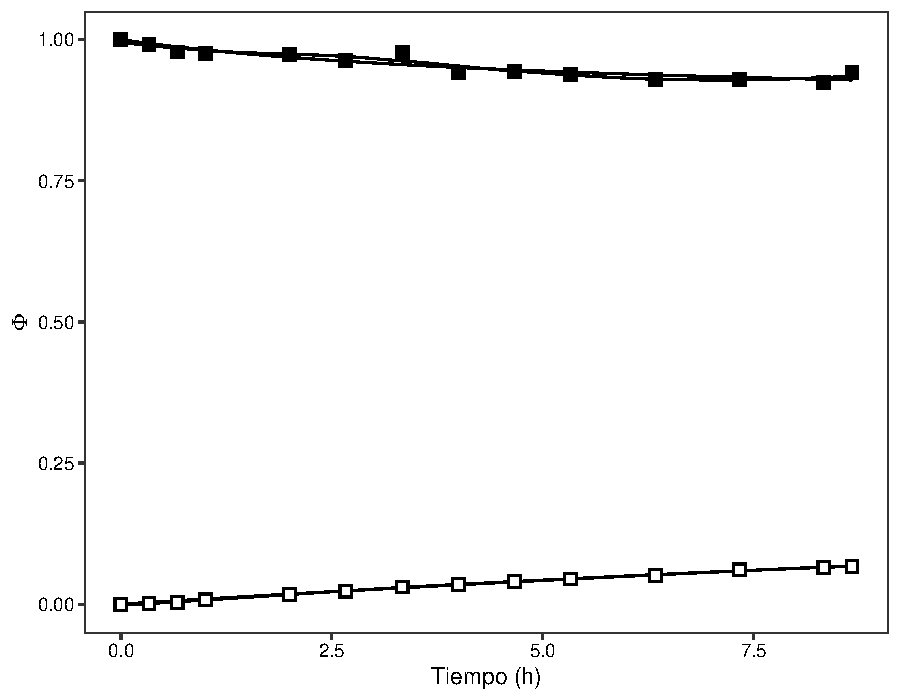
\includegraphics[height=0.388\textwidth]{chap5/figures/C1-profile.pdf}}
               \put(219, 168){\large a)}
               \end{picture}}%
    \subbottom{\begin{picture}(230,178)
               \put(0, 0){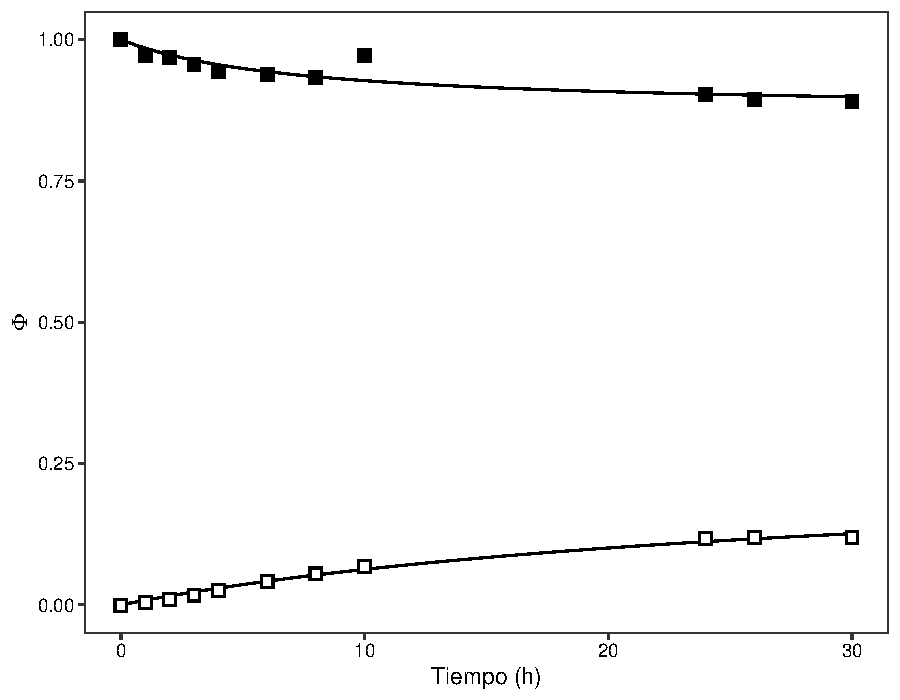
\includegraphics[height=0.388\textwidth, trim = {1.258cm 0 0 0},   clip]{chap5/figures/C2-profile.pdf}}
               \put(199, 168){\large b)}
               \end{picture}}
    \caption[Primeros perfiles de transporte de ion litio en celda de permeación.]{Perfiles de transporte de ion litio para las membranas C.1 (a) y C.2 (b). Fracción de ion litio en la fase de alimentación (\protect\squareblck) y fracción de ion litio en la fase de recuperación (\protect\squarewht). Disoluciones de alimentación: \ce{NaOH} 0.01~mol~kg\mnn, \ce{Li+} 18~mg~kg\mnn. Disolución recuperación (a): HCl 0.5~mol~kg\mnn. Disolución recuperación (b): HCl 1~mol~kg\mnn}        
    \label{fig:profileC1}
\end{figure}

\subsection{Primer diseño factorial fraccionado}\label{sec:FrF2-1}\index{Diseño de experimentos!factorial fraccionado}
Con el primer diseño experimental se pretendía encontrar el efecto a gran escala de la composición de la membrana y de las disoluciones de alimentación y de recuperación sobre la eficiencia del proceso de transporte. Se planteó una matriz de diseño factorial fraccionada de siete varia\-bles a dos niveles con resolución III. Las variables consideradas fueron las masas de polímero base (\textbf{X1}), plastificante (\textbf{X2}) y extractantes (\textbf{X3} y \textbf{X4} para LIX-54-100 y Cyanex~923, respectivamente) en la composición de la PIM, la concentración de hidróxido de sodio y de iones litio en la disolución de alimentación (\textbf{X5} y \textbf{X6}, respectivamente) y concentración de ácido clorhídrico en la fase de recuperación (\textbf{X7}). La respuesta (\textbf{Y}) fue la eficiencia del proceso de transporte de ion litio (ver Ecuación \ref{eq:efi}). La matriz de diseño y las respuestas de cada sistema se muestran en la Tabla \ref{tab:frf2matrix1}.  El diseño experimental fue creado y analizado usando el paquete \verb|FrF2| \citep{FrF2} de \verb|R-CRAN|.

\begin{table}[H]
    \centering\footnotesize
    \begin{tabular}{@{}ccccccccr@{}}\toprule
        \textbf{ID}& \textbf{X1} (mg)& \textbf{X2} (mg)& \textbf{X3} (mg)& \textbf{X4} (mg)& \textbf{X5} (mol~kg$^{-1}$)& \textbf{X6} (mg~kg\mnn)& \textbf{X7} (mol~kg\mnn) & \textbf{Y} (\%)\\\midrule
        D.1&30&   20&  12&     50&  0.001&    2&   0.1&2.4\\
        D.2&80&   20&  50&     12&  0.001&    2&   0.5&2.7\\
        \textbf{D.3}&\textbf{30}&   \textbf{40}&  \textbf{50}&     \textbf{12}&   \textbf{0.01}&    \textbf{2}&   \textbf{0.1}&\textbf{88.8}\\
        D.4&80&   20&  12&     12&   0.01&   10&   0.1&0.3\\
        D.5&80&   40&  50&     50&  0.001&   10&   0.1&0.0\\
        D.6&80&   40&  12&     50&   0.01&    2&   0.5&1.4\\
        D.7&30&   40&  12&     12&  0.001&   10&   0.5&0.3\\
        \textbf{D.8}&\textbf{30}&   \textbf{20}&  \textbf{50}&     \textbf{50}&   \textbf{0.01}&   \textbf{10}&   \textbf{0.5}&\textbf{22.2}\\\bottomrule
    \end{tabular}
    \caption{Matriz de diseño del primer diseño experimental factorial fraccionado.}
    \label{tab:frf2matrix1}
\end{table}


\begin{figure}[H]
    \centering
    \subbottom{\begin{picture}(245,178)
               \put(0, 0){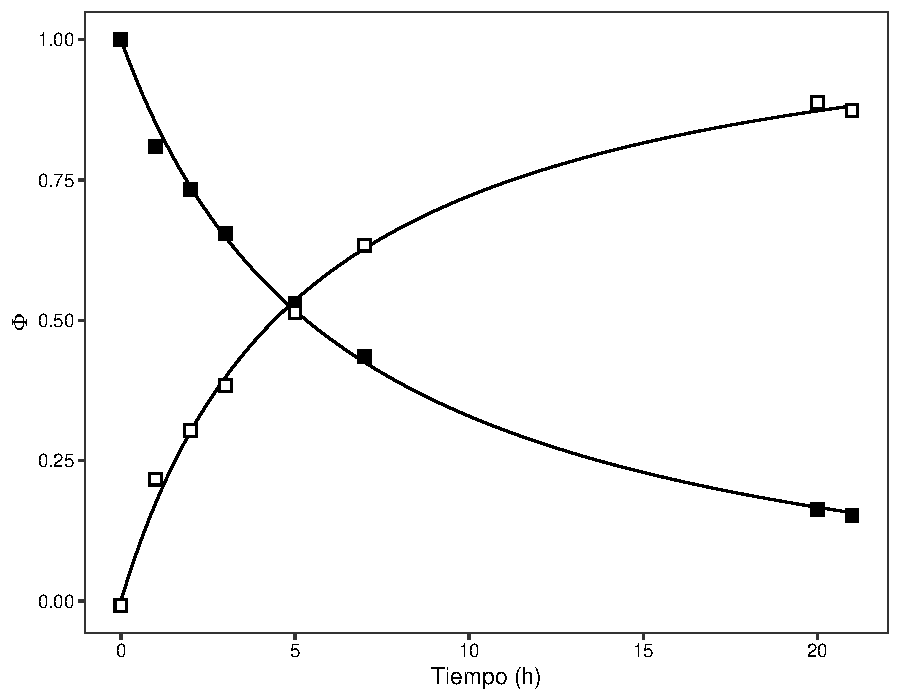
\includegraphics[height=0.388\textwidth]{chap5/figures/D3-profile.pdf}}
               \put(219, 167){\large a)}
               \end{picture}}%
    \subbottom{\begin{picture}(230,178)
               \put(0, 0){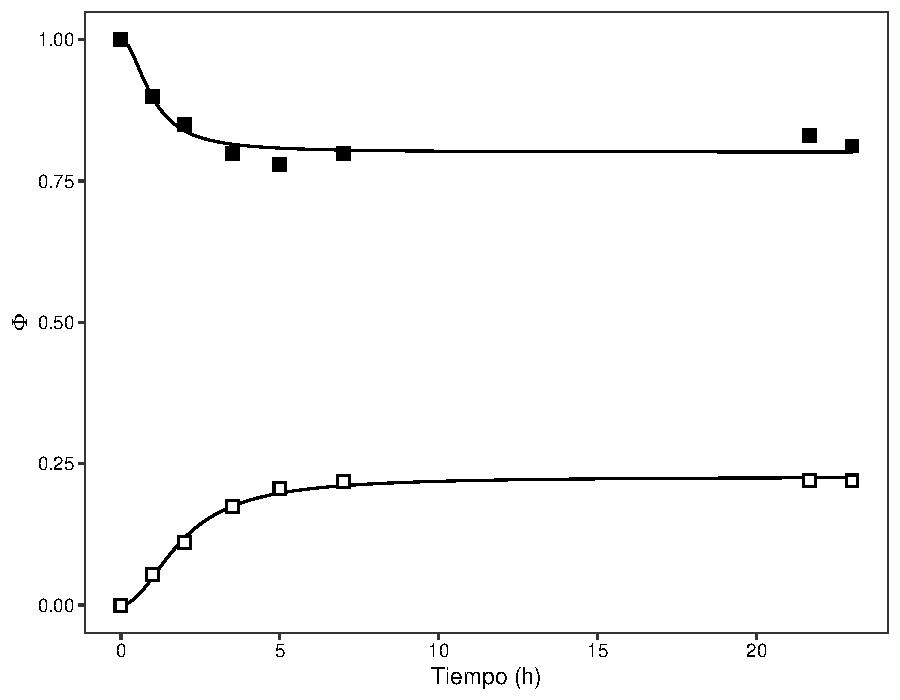
\includegraphics[height=0.388\textwidth, trim = {1.258cm 0 0 0},   clip]{chap5/figures/D8-profile.pdf}}
               \put(198, 167){\large b)}
               \end{picture}}
    \caption[Perfiles de transporte de ion litio membranas primer diseño factorial fraccionado.]{Perfiles de transporte de ion litio de los puntos 3 (a) y 8 (b) del primer diseño factorial fraccionado. Fracción de ion litio en la fase de alimentación (\protect\squareblck) y fracción de ion litio en la fase de recuperación (\protect\squarewht). Disolución de alimentación (a): NaOH 0.01~mol~kg\mnn, \ce{Li+} 2~mg~kg\mnn. Disolución de alimentación (b): NaOH 0.01~mol~kg\mnn, \ce{Li+} 10~mg~kg\mnn. Disolución de recuperación (a): HCl 0.1~mol~kg\mnn. Disolución de recuperación (b): HCl 0.5~mol~kg\mnn.}        
    \label{fig:FrF2_1.profiles}
\end{figure}

En la mayoría de los experimentos no se observa un transporte apreciable de ion litio hacia la diso\-lución de recuperación. Los perfiles de transporte de los únicos experimentos donde el ion litio fue transportado (PIM D.3 y PIM D.8) se muestran en la Figura \ref{fig:FrF2_1.profiles}. En el sistema que usa la PIM D.3 se observa que a las cinco horas de transporte el ion litio se encuentra a concentraciones iguales en ambas disoluciones y su transporte empieza a ocurrir en contra del gradiente de concentración. Este fue un avance importante en el desarrollo del método, dado que hasta el momento no se había observado el transporte activo del catión en cuestión.

La Figura  \ref{fig:FrF2-ME.1} muestra el gráfico de efectos principales del diseño experimental. Este gráfico muestra los contrastes de los factores estudiados y representa el efecto promedio de cada variable en la respuesta del sistema. Tomando como ejemplo la variable \textbf{X1} (masa de polímero base), la figura indica que los sistemas con 80~mg de CTA presentaron en promedio una eficiencia cercana a 0\% mientras los sistemas cuyas membranas tienen 30~mg de CTA presentaron en promedio una eficiencia de 28\%. 

El gráfico de efectos principales muestra que no se puede suponer la escasez de efectos. En ese orden de ideas los diagramas de Daniel no son apropiados para analizar los resultados del diseño experimental. Por otro lado, no se dispone de un estimador independiente de la variabilidad del método y esto imposibilita el uso de otras herramientas como el diagrama de Pareto. Bajo estas condiciones se dificulta mucho el análisis de los resultados del diseño por medio de herramientas {tradicionales} y puede concluirse que ninguna variable tiene un efecto importante en la respuesta del sistema dentro del intervalo de valores probados o bien, más probablemente, que la mayoría de las variables tienen una influencia significativa en el sistema. En diseños experimentales de cribado resulta peor ignorar la importancia de variables con efectos significativos que considerar como significativas a algunas variables no importantes \citep{FrF2}. Con base en esto, se decide analizar el gráfico de efectos principales en el modelo sin reducir.

\begin{figure}[H]
    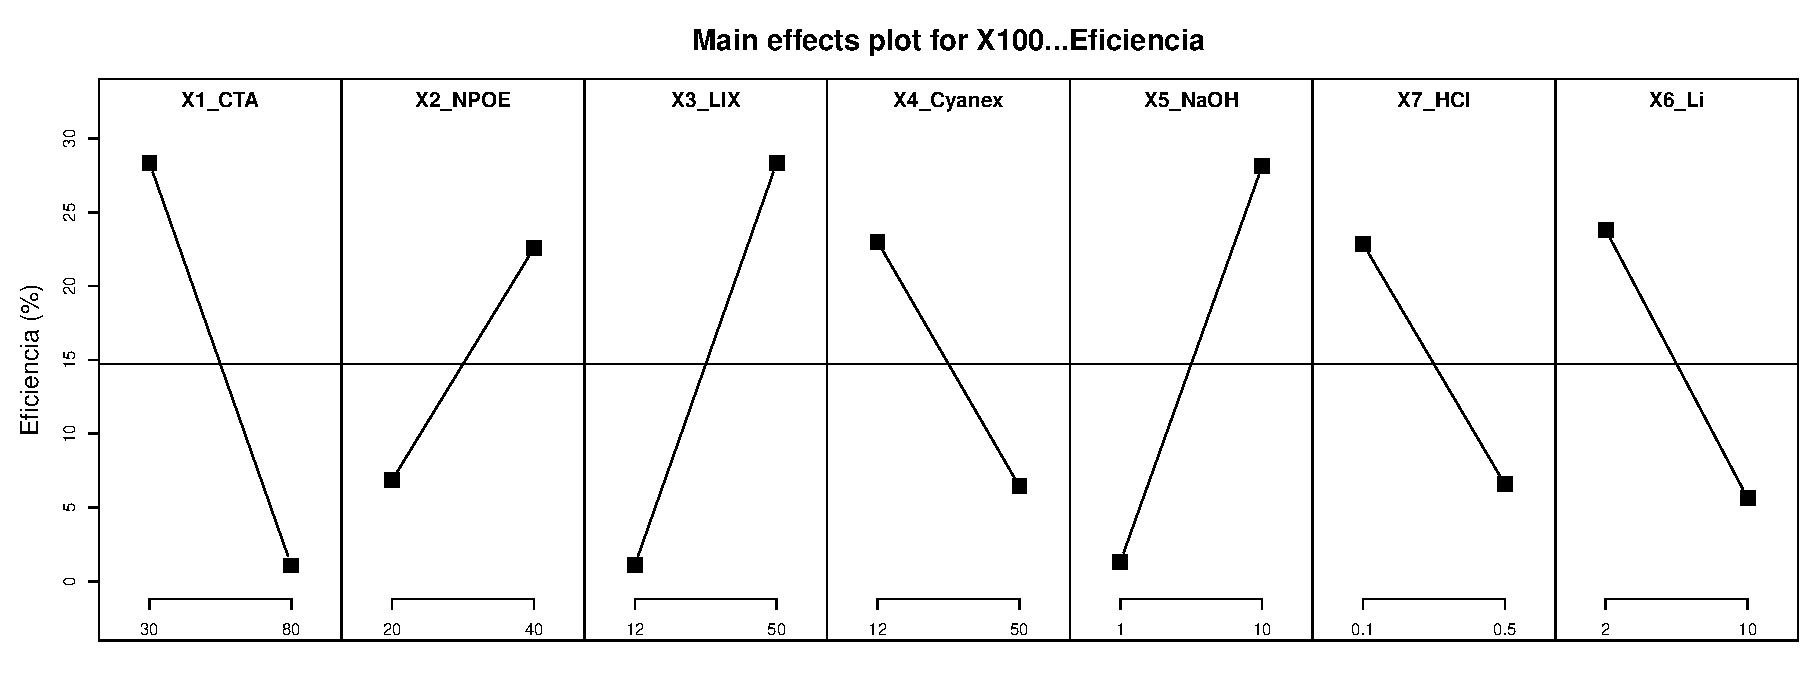
\includegraphics[width=\textwidth, trim = {0 1cm 0 1.34cm}, clip]{chap5/figures/MEP1.pdf}
    \caption[Gráfico de efectos principales del primer diseño factorial fraccionado.]{Gráfico de efectos principales del primer diseño factorial fraccionado. El eje de las abscisas que corresponde a la variable X5 (Concentración de hidróxido de sodio) ha sido multiplicado por 1000 para facilitar su visualización.}
    \label{fig:FrF2-ME.1}
\end{figure}

Los efectos de las variables son relativamente homogéneos, pero destacan ligeramente las masas de CTA y de LIX-54-100 en la membrana y la concentración inicial de hidróxido de sodio en la disolución de alimentación. Usando el método descrito en la Sección \ref{app:ParedesMethod}, el análisis de varianza de los modelos lineales simplificados univariados propuestos presentan \textit{valores p}  cercanos a 0.24 para las variables mencionadas. Esto indica que se carece de evidencia suficiente (con un 90\% de confianza) para aseverar que el efecto de modificar dichas variables en el intervalo considerado pueda distinguirse de la variabilidad propia del método. El resultado es similar cuando se analizan los modelos con las posibles combinaciones entre estas variables (por parejas y en terna) y carece de sentido intentar con las otras cuatro variables que presentan efectos principales inferiores en magnitud. 

Los resultados del diseño experimental no son suficientes para asegurar que el efecto de alguna variable en la eficiencia del sistema para extraer ion litio sea estadísticamente significativo. Debe tener\-se en cuenta que dicha conclusión está fuertemente influenciada por el hecho de que la mayo\-ría de las condiciones propuestas condujeron a procesos de transporte fallidos. Sin embargo, definitivamente algunas combinaciones de estas variables dan lugar a procesos de transporte significativamente mejores que algunas otras. El diagrama de efectos principales sugiere que un mejor transporte de iones litio se obtiene con una membrana de 30~mg de CTA, 40~mg de NPOE, 50~mg de LIX-54-100 y 12~mg de Cyanex~923, una disolución de alimentación de hidróxido de sodio 0.01~mol~kg\mnn\ y ion litio 2~mg~kg\mnn\ y una disolución de recuperación de ácido clorhídrico 0.1~mol~kg\mnn. Con base en esto, debe modificarse la metodología de análisis de los resultados y se considerará, simplemente, las condiciones bajo las cuales el transporte de ion litio fue posible a una escala apreciable (PIM D.3 y PIM D.8). 

Los sistemas PIM D.3 y PIM D.8 coinciden en que sus membranas contenían 30~mg de polímero base, 50~mg de LIX-54-100, y 0.01~mol~kg\mnn de hidróxido de sodio inicialmente en la fase de alimentación. El transporte es más eficiente cuando la concentración inicial de ion litio en la disolución de alimentación es pequeña, pues una menor cantidad de ion litio debe ser transportada a través de la membrana y la fracción transportada es mayor a tiempos menores. Una concentración inicial de ion litio en la fase de alimentación de 2~mg~kg\mnn\ presenta una ventaja adicional dado que, como se menciona en la Sección Anexa \ref{sec:liexternal}, la curva de calibración con patrones externos para ion litio por \ac{FAAS} presenta una buena linealidad hasta concentraciones de 2.5~mg~kg\mnn. Esto implica que si la disolución de alimentación contiene inicialmente 2~mg~kg\mnn\ de iones litio, no es necesario hacer diluciones para cuantificarlo. Las diluciones devengan tiempo valioso e introducen variación indeseada en los resultados para cuantificar la especie de interés. 

Respecto a la masa del extractante Cyanex~923, se observó que la elección de las variables \textbf{X3} y \textbf{X4} no fue la mas apropiada. Escoger la masa de cada extractante individualmente condujo a varias configuraciones en las que la relación molar entre estas especies era tan grande como 5.9:1 y tan pequeña como 0.34:1. Estos valores se encuentran muy alejados del reportado como óptimo por \citet{Pranolo2015}, y habría sido más conveniente utilizar como variables la masa total de extractantes y la relación molar entre estos. El perfil de transporte de la Figura \ref{fig:FrF2_1.profiles}(a)  sugiere que una masa de 12~mg de Cyanex~923 en la membrana produce transportes más eficientes, pero si se observa con detalle el sistema con la PIM D.8, se encuentra que la composición de membrana que contiene 100~mg de extractantes en relación molar 1.41:1 transporta una cantidad neta de ion litio mucho mayor en tiempos más cortos. Este valor de relación molar es similar al reportado por \citet{Pranolo2015}. Se sugiere que la relación molar óptima para el recobro de ion litio usando la PIM puede estar muy cerca de la reportada para el recobro de ion litio por \ac{SSX}.

Sobre la cantidad de plastificante en la membrana o la concentración inicial de ácido clorhídrico en la disolución de recuperación, no hay indicios que sugieran que un valor es mejor que el otro pero debió tomarse una decisión y con base en los buenos resultados del sistema PIM D.3 se escogieron 40~mg y 0.10~mol~kg\mnn, respectivamente.

Con base en lo discutido, se propuso una membrana con 30~mg de CTA, 40~mg de plastificante y 100~mg de una mezcla de extractantes LIX-54-100/Cyanex~923 en una relación molar 2:1. La concentración de hidróxido de sodio en la disolución de alimentación y de ácido clorhídrico en la disolución de recuperación para experimentos posteriores se fija en 0.01 y 0.1~mol~kg\mnn\, res\-pec\-tivamente. La concentración inicial de ion litio en las disoluciones de alimentación posteriores se mantuvo constante en 2~mg~kg\mnn.

\subsection{Efecto del plastificante en la eficiencia del transporte}\index{PIM!efecto del plastificante}
Las membranas preparadas hasta el momento han contenido siempre \ac{NPOE} como plastificante. Los plastificantes promueven modificaciones estructurales en las membranas y esto afecta su capacidad para el transporte de iones \citep{RodriguezdeSanMiguel2008}. En busca de una membrana capaz de transportar ion litio con una mayor rapidez, se compararon formulaciones con los plastificantes \ac{NPOE}, tris(2-etilhexil)fosfato (TEHP)\acused{TEHP}, tris(2-butoxietil)fosfato (TBEP) \acused{TBEP} y sin plastificante (membranas E.1, E.2, E.3 y E.4, respectivamente). La composición de las membranas y de las disoluciones empleadas fue la descrita al final de la sección anterior. Los perfiles de transporte obtenidos se muestran en la Figura \ref{fig:plasti1}.

\begin{figure}[htbp]
    \centering
    \subbottom{\begin{picture}(245,160)
               \put(0, 0){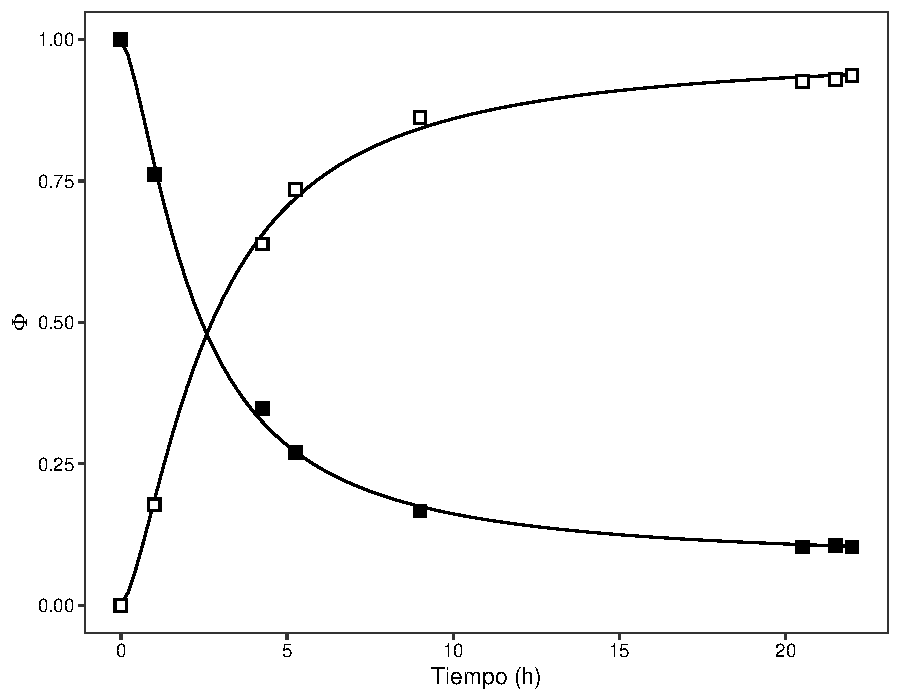
\includegraphics[height=0.355\textwidth, trim = {0 1cm 0 0},   clip]{chap5/figures/E.1-profile.pdf}}
               \put(218, 151.5){\large a)}
               \end{picture}}%
    \subbottom{\begin{picture}(230,160)
               \put(0, 0){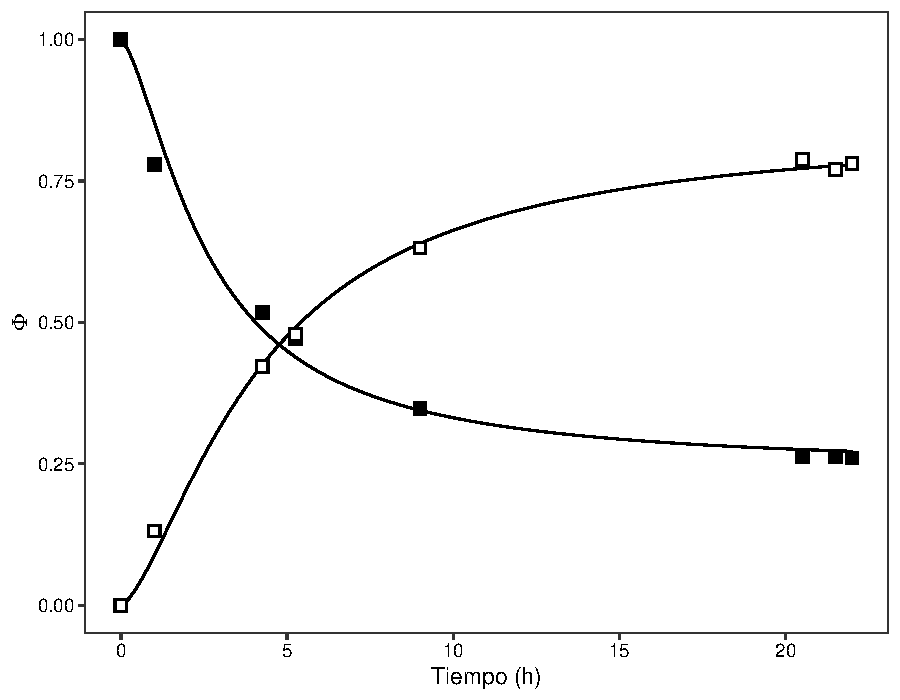
\includegraphics[height=0.355\textwidth, trim = {1.258cm 1cm 0 0},   clip]{chap5/figures/E.2-profile.pdf}}
               \put(197, 151.5){\large b)}
               \end{picture}}\\
    \subbottom{\begin{picture}(245,178)
               \put(0, 0){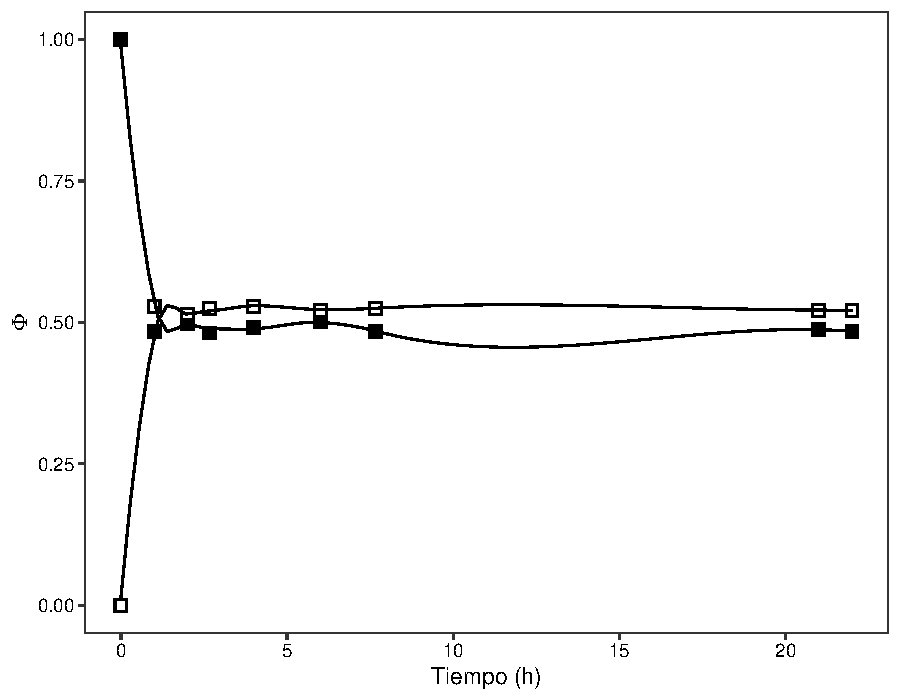
\includegraphics[height=0.388\textwidth]{chap5/figures/E.3-profile.pdf}}
               \put(218, 167){\large c)}
               \end{picture}}%
    \subbottom{\begin{picture}(230,178)
               \put(0, 0){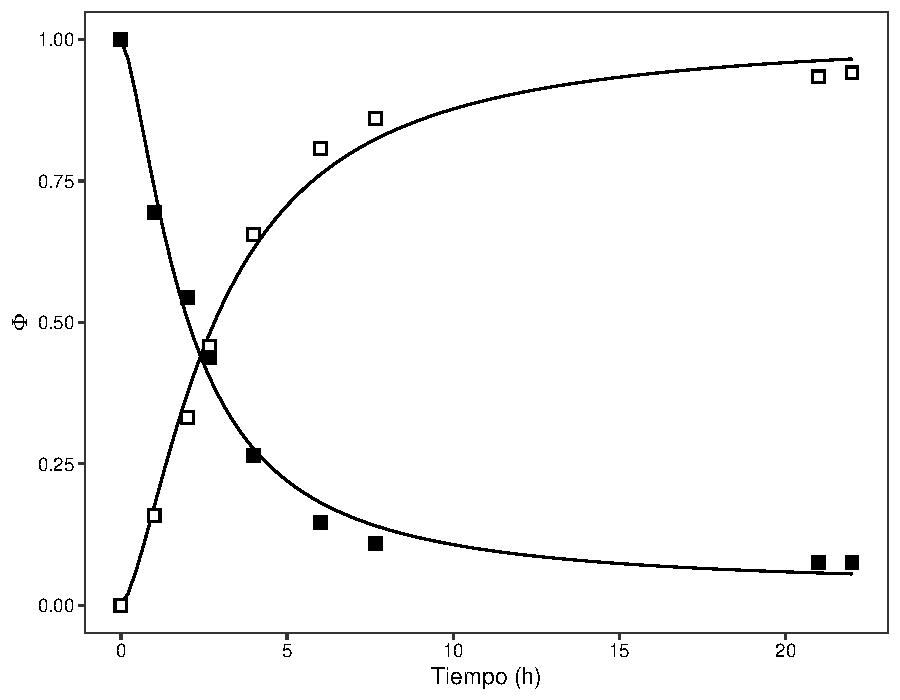
\includegraphics[height=0.388\textwidth, trim = {1.258cm 0 0 0},   clip]{chap5/figures/E.4-profile.pdf}}
               \put(197, 167){\large d)}
               \end{picture}}
    \caption[Perfiles de transporte de ion litio en membranas con distintos plastificantes.]{Perfiles de transporte de ion litio usando membranas sin plastificante (a), con NPOE (b), TEHP (c) y TBEP (d). Fracción de ion litio en la fase de alimentación (\protect\squareblck) y fracción de ion litio en la fase de recuperación (\protect\squarewht). Disoluciones de alimentación: NaOH 0.01~mol~kg\mnn, \ce{Li+} 2~mg~kg\mnn. Disoluciones de recuperación: HCl 0.1~mol~kg\mnn.}
    \label{fig:plasti1}
\end{figure}

La PIM que contiene \ac{TEHP} como plastificante posee pésimas propiedades mecánicas y se presentó una ruptura en la membrana. Las disoluciones de alimentación y de recuperación de este sistema se mezclaron y homogeneizaron como consecuencia de la agitación de las semiceldas. No fue posible observar transporte de ion litio mediado por la PIM. La concentración de ion litio en la disolución de recuperación para tiempos distintos de cero parece mayor a la determinada en la disolución de alimentación, pero esta diferencia no es importante y corresponde a que se usaron distintas curvas de calibración para compensar el efecto matriz en la cuantificación (ver Sección Anexa \ref{sec:liexternal}). 

La membrana sin plastificante presenta excelente desempeño. La eficiencia obtenida en el transporte de ion litio es del 94\%. Un desempeño similar se observa para la PIM con TBEP como plastificante en su composición. El NPOE confiere propiedades mecánicas aceptables a la membrana pero el desempeño de la misma es inferior respecto a las PIMs con TBEP o sin plastificante. Las propiedades mecánicas de la membrana sin plastificante fueron en general bastante buenas.

La principal función del plastificante en una PIM es mejorar su resistencia mecánica y su flexibilidad. Esto se logra por medio de la disminución de fuerzas intermoleculares entre las cadenas del polímero base. Una distancias media más grande entre las cadenas poliméricas ocasiona el ensanchamiento de la membrana \citep{Witt2018}. No incluir un plastificante adicional en la membrana evita un aumento en su grosor. Una membrana más delgada favorece el transporte de ion litio a través de la misma. La fabricación de PIMs sin plastificante que presentan buenas propiedades mecánicas y un buen desempeño para el transporte de diversas especies ha sido reportada por varios autores \citep{Vazquez2014, Xiong2019}. En estos casos, el extractante presenta doble función de extractante y plastificante.

%Entre los dos extractantes presentes en la PIM, el Cyanex~923 es probablemente el que hace también de plastificante. Distintos ésteres de ácido fosfórico han sido reportados como plastificantes de uso común en varios polímeros de uso industrial \citep{Wypych2017} pero no se encontraron reportes de óxidos de alquilfosfina usados para tal fin. \citet{Mead1942} reportaron que el tamaño y la forma de los plastificantes tiene una mayor influencia en su capacidad para plastificar que las particularidades de su estructura química. Los óxidos de alquilfosfinas tienen casi la misma cabeza polar que los ésteres de ácido fosfórico y esto los haría, \textit{grosso modo,} equivalentes como plastificantes a los esteres de ácido fosfórico con sustituyentes similares. Moléculas con cadenas alifáticas lineales (entre seis y ocho átomos de carbono para el caso del Cyanex~923) tienen mejores propiedades como plastificantes que moléculas con grupos cíclicos voluminosos (fenil en el caso del LIX-54-100) \citep{Mead1942}.

Un componente menos en la formulación de la PIM implica una variable menos que debe ser estudiada y optimizada. Esto a la vez se traduce en un costo de producción inferior que puede hacer más atractivo el escalamiento de la tecnología para una eventual aplicación industrial.
%\subsubsection{Primera optimización simplex}\label{sec:smplxexperimental1}
%Se buscó una mejora en el proceso de transporte por medio de una optimización siguiendo el algoritmo simplex modificado. Tras decidir que la membrana no llevaría plastificante en su composición (ver Sección \ref{sec:plasti1}), las variables consideradas fueron las masas de polímero base (\textbf{X1}) y de mezcla de extractantes (\textbf{X2}), la relación molar Lix-54-100/Cyanex923 en la mezcla (\textbf{X3}) y las concentraciones de hidróxido de sodio en la disolución de alimentación (\textbf{X4}) y de ácido clorhídrico en la disolución de recuperación. La variable respuesta ($\Upsilon$) se muestra en la ecuación \ref{ec:varUpsilon1}. 

%\begin{equation}\label{ec:varUpsilon1}
%    \Upsilon_i = \overline{\alpha_i}\cdot\overline{\beta_i}^{-1}
%\end{equation}
%donde $\overline{\alpha_i}$ y $\overline{\beta_i}$ son los parámetros de regresión (combinados) de la Ecuación \ref{eq:NLSCRIS} que describe los perfiles de transporte obtenidos en el \textit{i-}ésimo experimento (ver Sección \ref{sec:NLS}).

%El proceso de optimización se llevó a cabo con la ayuda del paquete \verb|labsimplex| del programa estadístico R  \citep{labsimplex}. Las coordenadas del punto inicial, el tamaño de paso y las coordenadas de los vértices del primer simplex se muestran en la Tabla \ref{tab:smplx1.1}.
%\begin{table}[H]
%    \centering\footnotesize
%    \begin{tabular}{@{}lccccc@{}}\toprule
%        \textbf{ID} & \textbf{X1} (mg) & \textbf{X2} (mg) & \textbf{X3} & \textbf{X4} (mol~kg\mnn\) & \textbf{X5} (mol~kg\mnn\) \\\midrule
%        \textit{Punto inicial} & 30 & 100 & 2.00 & 0.010 & 0.100\\
%        \textit{Tamaño de paso}& 10 &  20 & 1.00 & 0.005 & 0.050\\\midrule
%        F.1 \textit{(Vértice 1)}& 30&  100&    2.00& 0.010& 0.100\\
%        F.2 \textit{(Vértice 2)}&  40&   84&    2.00& 0.010& 0.100\\
%        F.3 \textit{(Vértice 3)}&  40&  104&    2.75& 0.010& 0.100\\
%        F.4 \textit{(Vértice 4)}&  40&  104&    1.75& 0.013& 0.100\\
%        F.5 \textit{(Vértice 5)}&  40&  104&    1.75& 0.008& 0.124\\
%        F.6 \textit{(Vértice 6)}&  40&  104&    1.75& 0.008& 0.074\\\bottomrule
%    \end{tabular}
%    \caption{Configuración y coordenadas del simplex de la primera optimización.}
%    \label{tab:smplx1.1}
%\end{table}

\subsection{Cambio de la base en la disolución de alimentación}
En el proceso de mejora de las condiciones para la extracción de ion litio se ha observado un dete\-rioro en la selectividad del sistema conforme se plantean condiciones que conducen a transportes más eficientes. Los iones sodio provenientes del hidróxido de sodio que se usa para alcalinizar la disolución de alimentación han sido identificados en la fase de recuperación cuando se cuantifica ion litio por \ac{FAAS}. Se observó que hasta un 25\% del sodio inicialmente presente en la disolución de alimentación puede ser cotransportado junto con el ion ion litio, y se decidió que era importante monitorear su proceso de transporte. 
%\begin{wrapfigure}{r}{0.55\textwidth}
%  \centering
%  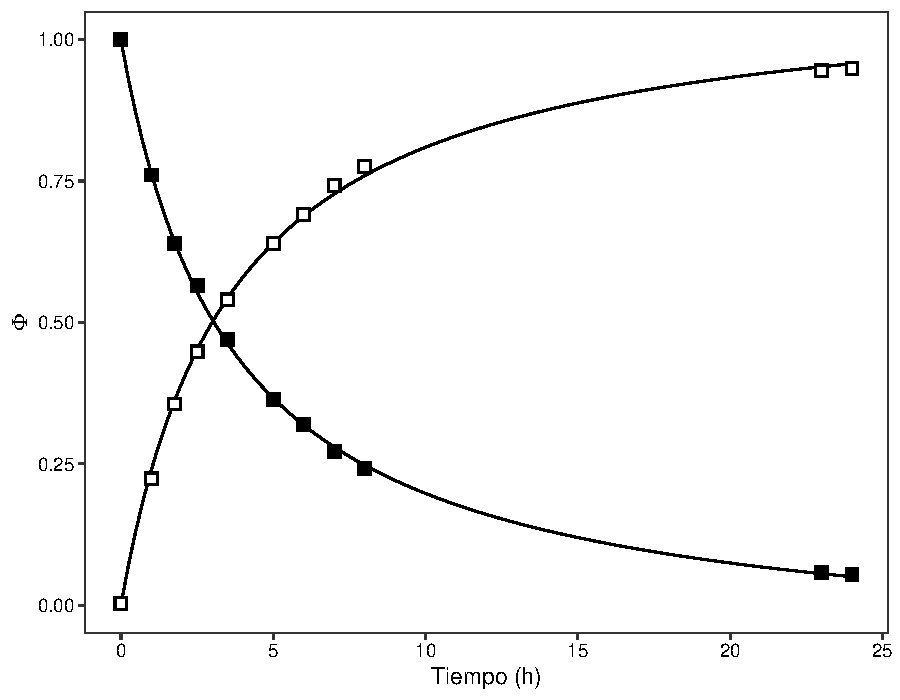
\includegraphics[height=0.388\textwidth]{chap5/figures/g1profile.pdf}
%  \caption{\vspace{-1ex}Perfil de transporte de ion litio usando hidróxido de amonio en la fase de alimentación.}
%  \label{fig:amonio1}
%\end{wrapfigure}

Se probó el reemplazo del hidróxido de sodio por hidróxido de amonio en la fase de alimentación para eliminar la omnipresencia de los iones sodio en todas las disoluciones de alimentación. Esto permitió estudiar el proceso de transporte cuando el ion litio es el único catión metálico en la fase de alimentación y permitió modificar sistemáticamente la concentración de los iones interferentes en esta disolución con el fin de facilitar el estudio de la selectividad de los sistemas. 

El perfil de transporte obtenido usando hidróxido de amonio 0.012~mol~kg\mnn\ en la fase de alimentación se muestra en la Figura \ref{fig:amonio1}. Puede observarse que la eficiencia en el transporte no disminuye como consecuencia del cambio de base, pero la velocidad a la que el ion litio es transportado a la fase de recuperación es menor que cuando se usa una base fuerte (hidróxido de sodio).
\begin{figure}[H]
  \centering
  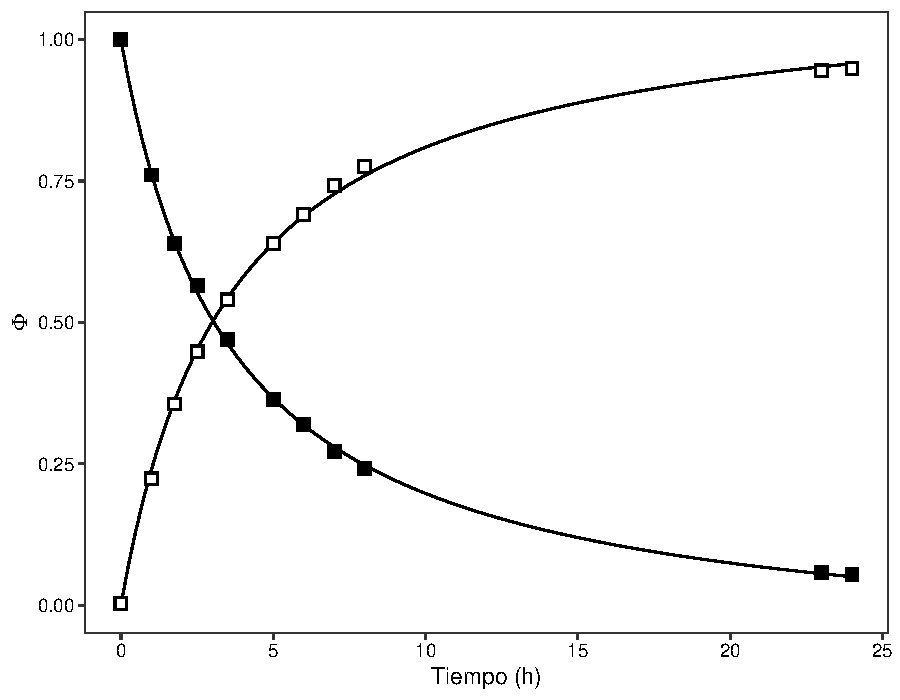
\includegraphics[height=0.388\textwidth]{chap5/figures/g1profile.pdf}
  \caption[Perfil de transporte de ion litio usando hidróxido de amonio en la fase de alimentación.]{Perfil de transporte de ion litio usando hidróxido de amonio en la fase de alimentación. Fracción de ion litio en la fase de alimentación (\protect\squareblck) y fracción de ion litio en la fase de recuperación (\protect\squarewht). Disolución de alimentación: \ce{NH4OH} 0.012~mol~kg\mnn, \ce{Li+} 2~mg~kg\mnn. Disolución de recuperación: HCl 0.1~mol~kg\mnn.}
  \label{fig:amonio1}
\end{figure}


\subsection{Segundo diseño factorial fraccionado}\index{Diseño de experimentos!factorial fraccionado}
En un nuevo diseño factorial fraccionado se pretendió encontrar condiciones para un transporte más rápido y eficiente, controlando la selectividad del sistema. Considerando la experiencia adquirida del diseño anterior, se escogieron las variables masa de polímero base (\textbf{X1}), masa de mezcla de extractantes (\textbf{X2}), relación molar LIX-54-100/Cyanex~923 en la mezcla de extractantes (\textbf{X3}) y las concentraciones de hidróxido de amonio en la disolución de alimentación (\textbf{X4}) y de ácido clorhídrico en la disolución de recuperación (\textbf{X5}). La matriz de diseño generada con el paquete \verb|FrF2| \citep{FrF2} se muestra en la Tabla \ref{tab:frf2matrix2}.

\begin{table}[H]
    \centering\footnotesize
    \begin{tabular}{@{}lccccc@{}}\toprule
        \textbf{ID}& \textbf{X1} (mg)& \textbf{X2} (mg)& \textbf{X3}& \textbf{X4} (mol~kg\mnn)& \textbf{X5} (mol~kg\mnn)
        \\\midrule
       H.1 & 30 &  70  &  2.0&    0.02 & 0.04\\
       H.2 & 45 &  70  &  3.5&    0.01 & 0.04\\
       H.3 & 30 & 110  &  3.5&    0.01 & 0.07\\
       H.4 & 45 &  70  &  2.0&    0.01 & 0.07\\
       H.5 & 45 & 110  &  3.5&    0.02 & 0.04\\
       H.6 & 45 & 110  &  2.0&    0.02 & 0.07\\
       H.7 & 30 & 110  &  2.0&    0.01 & 0.04\\
       H.8 & 30 &  70  &  3.5&    0.02 & 0.07\\\bottomrule
    \end{tabular}
    \caption{Matriz de diseño del segundo diseño experimental factorial fraccionado.}
    \label{tab:frf2matrix2}
\end{table}

Los procesos de transporte fueron monitoreados por 24 horas. La concentración de iones litio en la disolución de alimentación fue de 2~mg~kg\mnn. La selectividad de los sistemas fue evaluada respecto al transporte competitivo de iones sodio. Para esto, la disolución de alimentación contenía iones sodio en un exceso molar de 10:1 respecto al ion litio (concentración en masa iones sodio: 70~mg~kg\mnn). 

Se consideraron cuatro respuestas de manera independiente. Se tomaron los parámetros promediados $\alpha$ y $\beta$ de la regresión no lineal de los perfiles de transporte (Ecuación \ref{eq:NLSCRIS} de la Sección \ref{sec:NLS}) y el valor máximo del factor de separación litio/sodio ($Sf_{\ce{Li}/\ce{Na}}$). Las tres respuestas mencionadas fueron combinadas por medio de una función de deseabilidad \citep{Derringer} y fue considerada como una cuarta respuesta ($D$) que se analizó independientemente con el propósito de averiguar si es posible resumir todas las respuestas simultáneamente sin perder información relevante.\index{Diseño de experimentos!función deseabilidad}

En todos los experimentos se observó un transporte apreciable de iones litio. Los resultados se resumen en la Tabla \ref{tab:frf2results2}. Contrario a lo presentado en el anterior diseño experimental fraccionado (Sección \ref{sec:FrF2-1}), la respuesta más uniforme en los experimentos del presente conjunto permite un análisis más robusto considerando la significancia estadística del efecto de cada variable. 
\begin{table}[H]
    \centering\footnotesize
    \begin{tabular}{@{}ccccc@{}}\toprule
        \textbf{ID} & $\overline{\alpha}$ & $\overline{\beta}$ & $F_{\ce{Li}/\ce{Na}}$&$D$\\\midrule
        H.1 & 1.05 $\pm$ 0.01   & 0.96 $\pm$ 0.06   & 46.6 &0.67\\
        H.2 & 0.83 $\pm$ 0.01   & 0.15 $\pm$ 0.01   & 32.6 &0.00\\
        H.3 & 0.79 $\pm$ 0.01   & 0.59 $\pm$ 0.03   & 23.2 &0.00\\
        H.4 & 1.08 $\pm$ 0.01   & 0.29 $\pm$ 0.01   & 56.2 &0.47\\
        H.5 & 1.06 $\pm$ 0.02   & 0.63 $\pm$ 0.04   & 67.6 &0.79\\
        H.6 & 1.07 $\pm$ 0.01   & 0.29 $\pm$ 0.01   & 74.5 &0.56\\
        H.7 & 1.05 $\pm$ 0.01   & 0.78 $\pm$ 0.05   & 36.3 &0.53\\
        H.8 & 1.05 $\pm$ 0.01   & 0.62 $\pm$ 0.03   & 62.5 &0.74\\\bottomrule
    \end{tabular}
    \caption{Resultados segundo diseño experimental fraccionado.}
    \label{tab:frf2results2}
\end{table}

Los diagramas de Daniel para las cuatro variables respuesta se muestran en la Figura \ref{fig:DanielFrF2-2}. Las variables con efectos estadísticamente significativos se marcaron haciendo uso del método numé\-rico de \citet{Lenth1989} implementado en el paquete \verb|FrF2|. En estos diagramas aparece el efecto de la interacción entre las variables \textbf{X2:X3} y \textbf{X2:X5}. Las demás interacciones no aparecen debido a la estructura alias usada para generar la matriz de diseño. Las otras interacciones entre variables son alias (i.e. coinciden los contrastes y son obtenidos en conjunto) de alguna de las variables consideradas independientemente.

\begin{figure}[H]
    \centering
    \subbottom{\begin{picture}(240,138)
               \put(0, 0){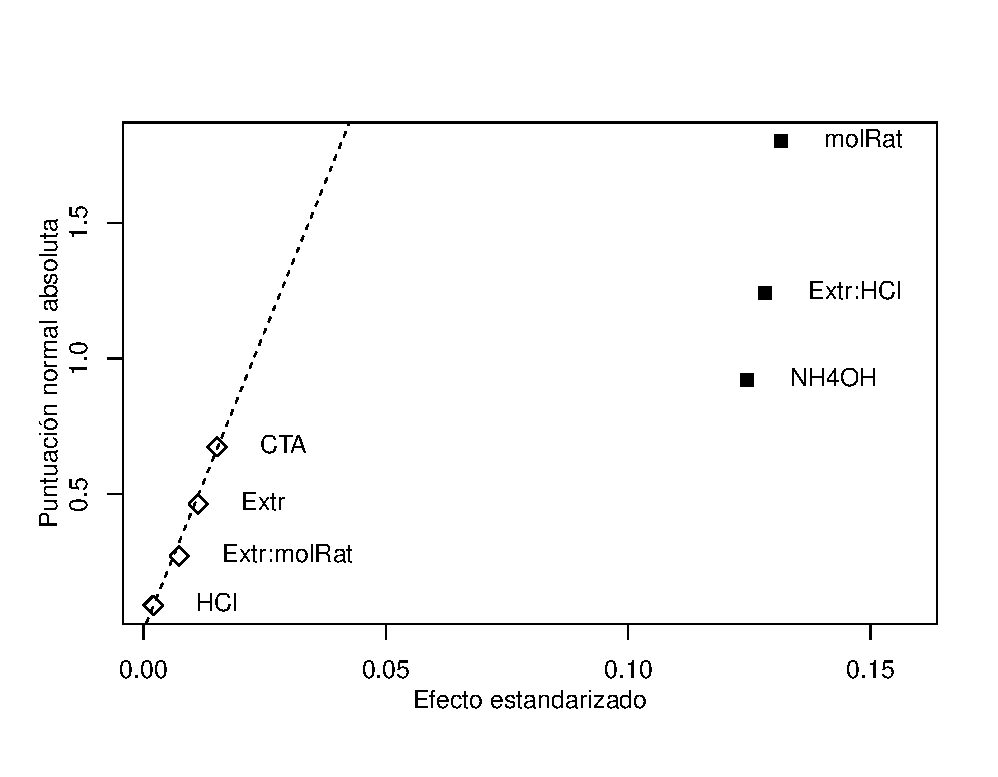
\includegraphics[height=0.355\textwidth, trim = {0 1.55cm 0 0},   clip, page = 1 ]{chap5/figures/DanielPlotsFrF2-2.pdf}}
               \put(32.8, 125){\large a)}
               \end{picture}}%
    \subbottom{\begin{picture}(230,138)
               \put(0, 0){\includegraphics[height=0.355\textwidth, trim = {1.92cm 1.55cm 0 0},   clip, page = 2 ]{chap5/figures/DanielPlotsFrF2-2.pdf}}
               \put(4.8, 125){\large b)}
               \end{picture}}\\
    \subbottom{\begin{picture}(240,138)
               \put(0, 0){\includegraphics[height=0.369\textwidth, page = 3, trim = {0 1.1cm 0 0},   clip ]{chap5/figures/DanielPlotsFrF2-2.pdf}}
               \put(32.8, 131){\large c)}
               \end{picture}}%
    \subbottom{\begin{picture}(230,138)
               \put(0, 0){\includegraphics[height=0.369\textwidth, trim = {1.92cm 1.1cm 0 0},   clip, page = 4 ]{chap5/figures/DanielPlotsFrF2-2.pdf}}
               \put(4.8, 131){\large d)}
               \end{picture}}
    \caption[Diagramas de Daniel del segundo diseño factorial fraccionado.]{Diagramas de Daniel del segundo diseño factorial fraccionado para las diferentes respuestas consideradas: Parámetro promediado $\alpha$ (a), parámetro promediado $\beta$ (b), coeficiente de separación (c) y función de deseabilidad (d). Variables con efectos estadísticamente significativos (\protect\squareblck) y variables cuyo efecto no puede diferenciarse del mero error aleatorio (\protect\squarerttdwht).}
    \label{fig:DanielFrF2-2}
\end{figure}

Puede observarse en la Figura \ref{fig:DanielFrF2-2}(d) que el análisis de los resultados a través de la función de deseabilidad logra resumir la mayoría de las conclusiones que pueden obtenerse considerando las variables respuesta cada una por separado. La única excepción se presenta con la variable de masa polímero base en la membrana (\textbf{X1}, CTA), que según la Figura \ref{fig:DanielFrF2-2}(b) tiene un efecto estadísticamente significativo sobre el parámetro $\beta$ que se relaciona con la rapidez a la que ocurre el proceso de transporte. El efecto de esta variable no ha resultado estadísticamente significativo cuando el análisis se hace usando la función deseabilidad.

El efecto de las variables que se han encontrado como estadísticamente significativas puede ser observado en un gráfico de efectos principales similar al mostrado en la Figura \ref{fig:FrF2-ME.1}. Sin embargo, una de las interacciones que no se encuentra confundida con ningún efecto principal ha sido encontrada como relevante según los diagramas de Daniel y el método de Lenth. En este caso es más apropiado visualizar los resultados en un gráfico de interacciones. El gráfico de interacciones permite el estudio los efectos principales proyectados en dos dimensiones para contemplar los contrastes de todas las variables combinadas entre sí. En este gráfico las variables que no tienen interacción se muestran como líneas paralelas, las variables que tienen efectos sinérgicos se muestran como líneas no paralelas pero con pendiente de signo igual, y las variables que tienen interacción total se muestran como líneas rectas que tienen pendientes de signo opuesto.

El gráfico de interacciones, usando la función de deseabilidad como respuesta se muestra en la Figura \ref{fig:IAPLOTFrF2-2}.  

\begin{figure}[H]
    \centering
    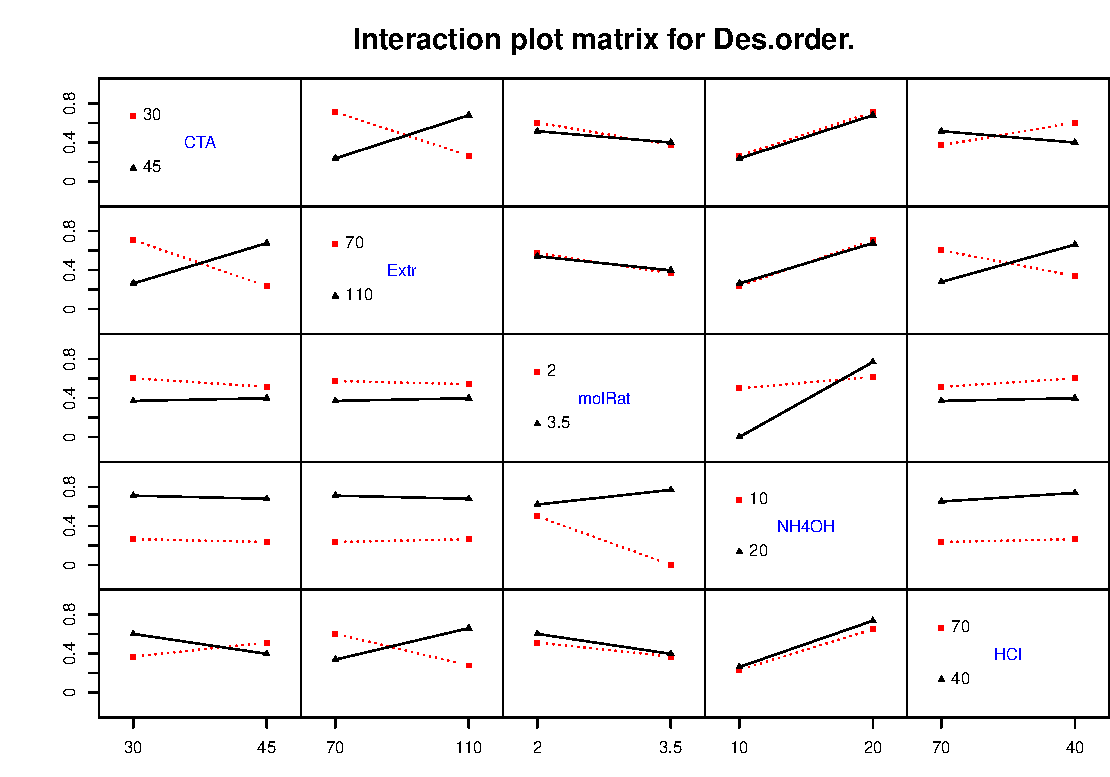
\includegraphics[width=0.9\textwidth, trim={1cm 0.3cm 0 1cm}, clip]{chap5/figures/IAPlotFrF2-2.pdf}
    \caption[Gráfico de interacciones del segundo diseño factorial fraccionado.]{Gráfico de interacciones de las variables consideradas en el segundo diseño factorial fraccionado. Los ejes de las abscisas que corresponden a las variables X4 y X5 (concentración de hidróxido de sodio y de ácido clorhídrico) han sido multiplicados por 1000 para facilitar su visualización.}
    \label{fig:IAPLOTFrF2-2}
\end{figure}

De la forma de las rectas de la Figura \ref{fig:IAPLOTFrF2-2}, considerando los diagramas de Daniel presentados anteriormente para tener en cuenta únicamente las variables cuyo efecto ha resultado estadísticamente significativo, se deduce lo siguiente:
\begin{itemize}
    \item Una concentración inicial de 0.02~mol~kg\mnn\ de hidróxido de amonio en la disolución de alimentación se traduce en procesos de transporte más eficientes y más selectivos.
    \item Los transportes son más eficientes usando membranas con una relación molar de extractantes LIX-54-100/Cyanex~923 de 2 que cuando se usa 3.5.
    \item Con el diagrama de efectos principales para la variable respuesta $\beta$ (no mostrado acá) se deduce que membranas con 30~mg de polímero base conducen a transportes más rápidos que cuando se usan 45~mg. Esto es lógico considerando que el grosor de la membrana está fuertemente influenciado por la cantidad de polímero base que lleva. Membranas más gruesas implican una región mayor del espacio que debe atravezar el ion litio para llegar a la fase de recuperación. Membranas con menos de 30~mg de CTA fueron preparadas para obtener transportes más rápidos, pero una cantidad de polímero base tan pequeña no provee del soporte y la resistencia mecánica suficiente para que la membrana resulte de alguna utilidad.
    \item El efecto de la masa total de extractantes en la membrana depende de la concentración inicial de ácido en la disolución de recuperación. Los transportes en los que se usan membranas con una masa de mezcla de extractantes pequeña (70~mg) son más eficientes si la concentración inicial de ácido en la disolución de recuperación es de 0.07~mol~kg\mnn\ (respecto a cuando se usa 0.04~mol~kg\mnn). Lo contrario se observa cuando se usan masas mayores de extractantes en la composición de la membrana.
\end{itemize}

La Tabla \ref{tab:paredesFrF2-2} contiene el resumen de los resultados obtenidos al usar el método propuesto descrito en la Sección \ref{app:ParedesMethod} para determinar que variables resultaron tener un efecto estadísticamente significativo sobre las cuatro respuestas consideradas. Los resultados del método se muestran como las variables cuyo valor p es inferior a la significancia escogida (0.10) en al menos uno de los análisis de varianza efectuados sobre los distintos modelos lineales que consideran un distinto número de variables explicatorias a la vez. El análisis se hace para cada respuesta con el fin de comparar las conclusiones que pueden obtenerse por este método con las obtenidas en párrafos anteriores.

\begin{table}[H]
    \centering\footnotesize
    \begin{tabular}{@{}llll@{}}\toprule
        \multirow{2}{*}{\textbf{Respuesta}} & \textbf{Número de} & \textbf{Variables} & \multirow{2}{*}{\textbf{Valores P}} \\
        &\textbf{variables} &\textbf{significativas}\\\midrule
        Parámetro $\alpha$ & 1 & - & -\\
                           & 2 & X3, X4 & 0.07, 0.08\\
                           & 3 & - & -\\
                           & 4 & - & - \\
                           & 5 & - & - \\\midrule
        Parámetro $\beta$  & 1 & X1 & 0.02\\
                           & 2 & X1 & 0.03\\
                           & 3 & X1 & 0.05\\
                           & 4 & X1 & 0.06\\
                           & 5 & X1 & 0.06 \\\midrule
        Factor de separación & 1 & X4 & 0.03\\
                             & 2 & X4 & 0.05\\
                             & 3 & X1, X4 & 0.09, 0.07\\
                             & 4 & X1, X4 & 0.10, 0.06\\
                             & 5 & X4 & 0.09\\\midrule
        Función de deseabilidad & 1 & X4 & 0.03\\
                                & 2 & X4 & 0.04\\
                                & 3 & X4 & 0.07\\
                                & 4 & X4 & 0.06\\
                                & 5 & - & - \\\bottomrule
    \end{tabular}
    \caption[Variables con efectos estadísticamente significativos.]{Variables con efectos estadísticamente significativos según el nuevo método propuesto.}
    \label{tab:paredesFrF2-2}
\end{table}
No se incluyó la interacción entre pares de variables dado que la estructura alias de la matriz de diseño involucra la superposición de varios efectos individuales con la interacción entre varios pares de variables. Esto implica que varias interacciones entre parejas de variables pueden ser erróneamente interpretadas a menos que se trate de las variables \textbf{X2:X3} y \textbf{X2:X5} que se evaluaron en ausencia de la sobreposición de efectos de variables individuales. Esto presenta una posible pérdida valiosa de información que puede solucionarse si se incluyen solo las interacciones libres de estructuras alias, pero no se encontró una forma automática de hacer esto.

Las variables explicatorias que han resultado estadísticamente significativas para las distintas respuestas coinciden en su mayoría con las que han sido seleccionadas usando el diagrama de Daniel en conjunto con el método de Lenth. Las excepciones las presentan las variables respuesta \textbf{Y3} ({selectividad}) y \textbf{Y4} ({función de deseabilidad}). Para la función de deseabilidad solo se ha identificado como relevante la concentración inicial de hidróxido de amonio en la disolución de alimentación mientras el efecto de la relación molar de los extractantes no ha podido ser diferenciado de la variación propia del método a un nivel de confianza del 90\%. Respecto a la selectividad del método, la masa de CTA en la membrana parece tener un efecto estadísticamente significativo que es contrario al encontrado para la velocidad del proceso (parámetro $\beta$). Probablemente, membranas más gruesas afectan en mayor proporción al transporte de cationes interferentes que al transporte de iones litio.

Con las conclusiones obtenidas se propone una composición de la \ac{PIM} con 30~mg de polímero base y 70~mg de mezcla de extractantes LIX-54-100/Cyanex~923 en relación molar 2:1, una concentración inicial de hidróxido de amonio en la disolución de alimentación de 0.02~mol~kg\mnn\ y una concentración inicial de ácido clorhídrico en la disolución de recuperación de 0.07~mol~kg\mnn.

\subsection{Condiciones hidrodinámicas y reproducibilidad}\label{sec:reprod}
Los perfiles de transporte de ion litio hacia la disolución de recuperación para distintos valores de rapidez de rotación de la propela en el compartimiento de la disolución de alimentación se muestran en la Figura \ref{fig:RPM1}(a). La fracción de ion litio transportada al final del proceso de transporte en función de la rapidez de rotación se muestra en la Figura \ref{fig:RPM1}(b). 

\begin{figure}[H]
    \centering
    \subbottom{\begin{picture}(240,167)
               \put(0, 0){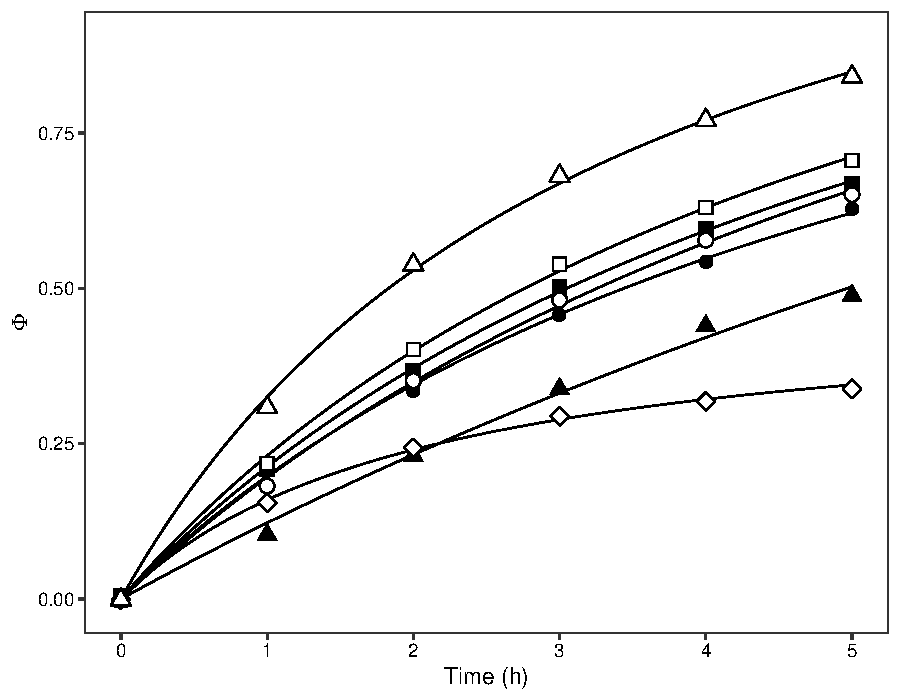
\includegraphics[height=0.375\textwidth, trim = {0 0 0 0},   clip]{chap5/figures/Thetha1_profiles.pdf}}
               \put(23, 160){\large a)}
                \end{picture}}%
    \subbottom{\begin{picture}(190,167)
               \put(0, 0){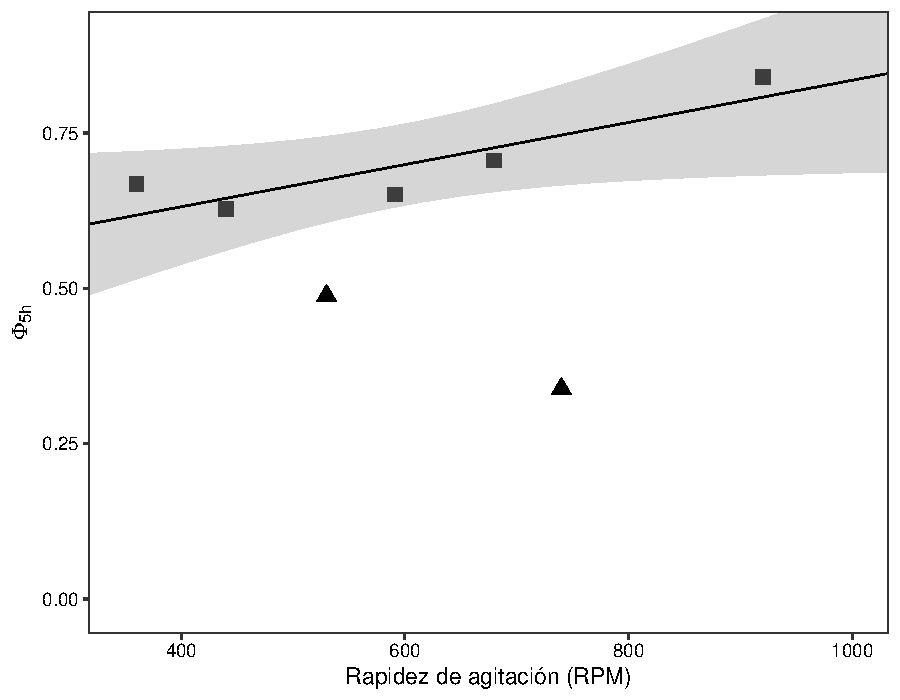
\includegraphics[height=0.375\textwidth, trim = {1.35cm 0 0 0},   clip]{chap5/figures/RPM_1.pdf}}
               \put(5, 160){\large b)}
               \end{picture}}\\
    \caption[Efecto de las condiciones hidrodinámicas en el proceso de transporte.]{Efecto de las condiciones hidrodinámicas en el proceso de transporte: (a) Perfiles de transporte de ion litio a distintos valores de rapidez de agitación (\protect\squareblck\ 360, \protect\circleblck\ 440, \protect\triangleupblck\ 530, \protect\circlewht\ 591, \protect\squarewht\ 680, \protect\squarerttdwht\ 740 y \protect\triangleupwht\ 920 RPM) y (b) fracción transportada de ion litio a las cinco horas en función de la rapidez de agitación (\protect\triangleupblck\ datos excluídos en la regresión). La zona sombreada corresponde al intervalo de confianza de la regresión a un nivel de confianza del 95\%. Disoluciones de alimentación: \ce{NH4OH} 0.02~mol~kg\mnn, \ce{Li+} 2~mg~kg\mnn. Disoluciones de recuperación: HCl 0.07 mol~kg\mnn.}
    \label{fig:RPM1}
\end{figure}

No parece haber una correlación fuerte entre la rapidez de agitación y la eficiencia del proceso de transporte. Si se excluyen los valores obtenidos a 530 y 740 RPM la relación es estadísticamente significativa (valor p de la prueba F sobre el modelo de regresión: 0.048), pero la distribución de los residuales de la regresión no es aleatoria, lo que indica que el modelo no describe adecuadamente el comportamiento de los datos. 

En principio, se esperaría que un aumento en la rapidez de agitación tenga un efecto positivo en la rapidez a la que el ion litio es transportado a través de la membrana hasta alcanzar un valor límite a partir del cual la rapidez de agitación no influye en la cinética del proceso. Esto se supone considerando que una rapidez de giro mayor en la propela hace más eficiente la homogeneización del seno de la disolución disminuyendo el grosor de la capa de difusión que deben atravesar las especies para llegar a la interfaz disolución-membrana. A partir de un valor límite, el grosor de la capa de difusión no puede disminuir más y la cinética del proceso queda controlada únicamente por la rapidez de la reacción interfacial de complejación y la velocidad a la que el aducto que se forma es transportado al otro lado de la membrana. 

En el gráfico de la Figura \ref{fig:RPM1}(b) no se observa ninguna región estacionaria. El transporte ineficiente que se obtuvo a 740 RPM puede justificarse por la formación de un régimen turbulento que es difícil de controlar a altos valores de $\Theta$. El efecto de la agitación parece no tener gran importancia en el intervalo de valores de rapidez de agitación entre 400 y 680 RPM.

Se evaluó la reproducibilidad del proceso agitando las semiceldas a valores entre 510 y 585 \ac{RPM}. Los perfiles de transporte de ion litio y los factores de separación respecto al sodio se muestran en la Figura \ref{fig:RPM2}. Se bloqueó la variable {celda de transporte} (Celda 1 y 2) y se aleatorizó la variable {rapidez de agitación} ($\Theta$).

\begin{figure}[H]
    \centering
    \subbottom{\begin{picture}(240,167)
               \put(0, 0){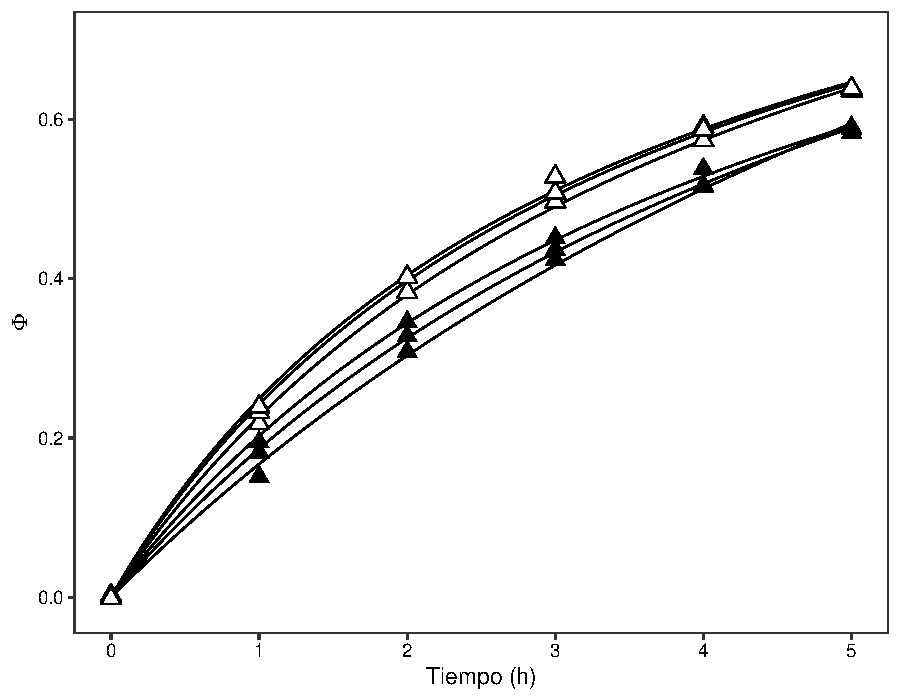
\includegraphics[height=0.37\textwidth, trim = {0cm 0 0 0},   clip]{chap5/figures/Theta2_profiles.pdf}}
               \put(0, 161){\large a)}
               \end{picture}}%
    \subbottom{\begin{picture}(250,167)
               \put(0, 0){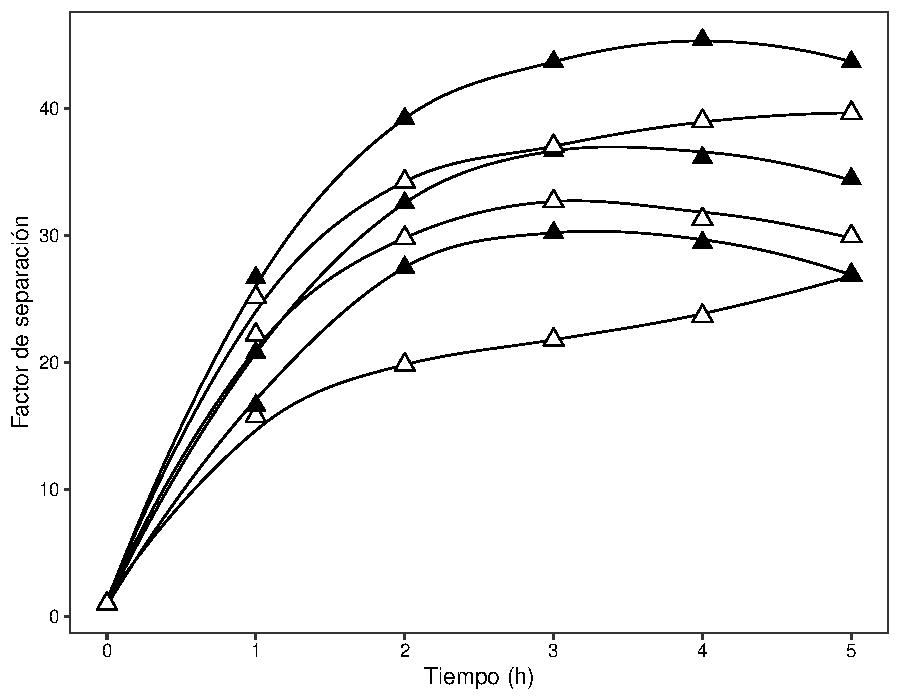
\includegraphics[height=0.37\textwidth, trim = {0cm 0 0 0},   clip]{chap5/figures/SepFactor_Thetha2.pdf}}
               \put(0, 161){\large b)}
               \end{picture}}\\
    \caption[Reproducibilidad del proceso de transporte.]{Reproducibilidad del proceso de transporte: (a) Perfiles de transporte de ion litio a la disolución de alimentación  y (b) factor de separación en función del tiempo para los distintos sistemas en la Celda 1 (\protect\triangleupblck) y en la Celda 2 (\protect\triangleupwht). Disoluciones de alimentación: \ce{NH4OH} 0.02~mol~kg\mnn, \ce{Li+} 2~mg~kg\mnn. Disoluciones de recuperación: HCl 0.07 mol~kg\mnn.}
    \label{fig:RPM2}
\end{figure}

Hay diferencias estadísticamente significativas\footnote{A un valor de confianza del 95\%. Valor p de la prueba t de igualdad de medias sobre la fracción transportada de ion litio a las cinco horas: 0.002} entre los transportes realizados en la celda 1 o en la celda 2. Los factores de separación presentan una gran variabilidad que parece ser independiente de la celda en la que se lleva a cabo el transporte y de la rapidez con la que se agiten las semiceldas. La desviación estándar relativa de la fracción transportada de ion litio a la disolución de alimentación está entre 15\% y 5\% para tiempos de una y cinco horas, respectivamente. La desviación estándar relativa del factor de separación es de 20\% y se mantiene relativamente contante en el tiempo. Considerando en conjunto los transportes realizados en cada celda, la desviación estándar relativa de los parámetros $\alpha$ y $\beta$ es de alrededor del 5\% (con la excepción del parámetro $\beta$ para los transportes en la celda 1 que es del 20\%). 

Se decidió trabajar únicamente con la celda 2 para los demás experimentos de transporte. La celda 1 se descontrolaba con frecuencia, produciendo derrames y haciendo más desgastantes la supervisión de los experimentos. Adicionalmente, los transportes de ion litio realizados en la celda 2 fueron más eficientes. 
 
%\subsubsection{Tercer diseño factorial fraccionado}
%En un intento por mejorar la eficiencia y la selectividad del sistema modificando algunas variables categóricas, se desarrollo un tercer diseño factorial fraccionado en el que se evaluaron tres parámetros: disolvente empleado en la preparación de la membrana (\textbf{X1}), morfología de la caja de petri usada como molde (\textbf{X2}). y disolución expuesta a la cara rugosa de la membrana (\textbf{X3}). La matriz de diseño se muestra en la Tabla \ref{tab:frf2matrix3}. Las membranas y las disoluciones de alimentación y de recuperación utilizadas son de la misma composición que las utilizadas en la Sección \ref{sec:hydroexpe}


%\subsubsection{Reproducibilidad del sistema}
%Previa a la optimización final del sistema es necesario conocer la reproducibilidad del mismo para establecer que diferencias en los resultados pueden considerarse importantes estadísticamente. Idealmente este proceso tuvo que haberse hecho antes del estudio del sistema haciendo uso de los experimentos factoriales fraccionados descritos en secciones anteriores.

\subsection{Optimización simplex}\index{Diseño de experimentos!algoritmo símplex}
Para optimizar el sistema se consideraron las variables masa de mezcla de extractantes (\textbf{X1}), relación molar LIX-54-100/Cyanex~923 (\textbf{X2}), concentración inicial de hidróxido de amonio en la disolución de alimentación (\textbf{X3}) y concentración inicial de ácido clorhídrico en la disolución de recuperación (\textbf{X4}). La masa de \ac{CTA} en las membranas se mantuvo constante en 30~mg. El objetivo de la optimización fue aumentar la velocidad del proceso de transporte, por lo que se consideró la maximización del parámetro promediado $\beta$ de los perfiles de transporte modelados usando la Ecuación \ref{eq:NLSCRIS} propuesta en el Capítulo \ref{sec:NLS}.

Para monitorear el factor de separación, se dispuso cloruro de sodio en la disolución de alimentación a una concentración tal que la relación molar \ce{Li+}/\ce{Na+} fuese de 1:10. El punto inicial del simplex y el tamaño de paso configurado se muestran en la Tabla \ref{tab:smplx2.1}. En la misma tabla se incluyen las coordenadas del simplex inicial generado junto con la respuesta obtenida para cada punto.

\begin{table}[H]
    \centering\footnotesize
    \begin{tabular}{@{}l c c c c c@{}}\toprule
         \textbf{ID}&\textbf{X1} (mg)&\textbf{X2}&\textbf{X3} (mol~kg\mnn)&\textbf{X4} (mol~kg\mnn)&$\overline{\beta}$\\\midrule
        \textit{Punto inicial}  & 70& 2.00& 0.010& 0.07&-\\
        \textit{Tamaño de paso} & 20 & 1.00& 0.010& -0.06&-\\\midrule
        \textbf{K.1} \textit{(vértice 1)}& \textbf{70.0}& \textbf{2.00}& \textbf{0.010}& \textbf{0.07}& \textbf{0.487}\\
        K.2&  50.0& 2.75& 0.010& 0.07& 0.397\\
        K.3&  50.0& 1.75& 0.016& 0.07& 0.254\\
        K.4&  50.0& 1.75& 0.007& 0.04& 0.268\\
        K.5&  50.0& 2.75& 0.007& 0.04& 0.345\\\bottomrule
    \end{tabular}
    \caption{Configuración del simplex inicial.}
    \label{tab:smplx2.1}
\end{table}

El proceso de optimización se completó con los puntos que se muestran en la Tabla \ref{tab:smplx2.2}. Los perfiles de transporte correspondientes al primer vértice (punto inicial de la optimización) y al vértice con la mejor respuesta (PIM K.9) se muestran en la Figura \ref{fig:simplex2.profiles}.
\begin{table}[H]
    \centering\footnotesize
    \begin{tabular}{@{}l l c c c c c@{}}\toprule
         \textbf{ID}&\textbf{Movimiento}&\textbf{X1} (mg)&\textbf{X2}&\textbf{X3} (mol~kg\mnn)&\textbf{X4} (mol~kg\mnn)&$\overline{\beta}$\\\midrule
         K.6&R&  60.0 & 2.88& 0.000& 0.04& 0.000\\
         K.7&Cw&  52.5& 2.03& 0.012& 0.06& 0.434\\
         K.8&R&  61.2& 3.02& 0.013& 0.08& 0.424\\
         \textbf{K.9}&\textbf{R}&  \textbf{66.8}& \textbf{2.15}& \textbf{0.016}& \textbf{0.10}& \textbf{0.554}\\
        K.10& E& 75.3& 1.85& 0.020& 0.13& 0.343\\
        K.11& R& 75.3& 1.85& 0.016& 0.09& 0.388\\
        K.12& Cw&56.3& 2.52& 0.011& 0.07& - \\\bottomrule
    \end{tabular}
    \caption{Vértices generados en el proceso de optimización.}
    \label{tab:smplx2.2}
\end{table}

\begin{figure}[H]
    \centering
    \subbottom{\begin{picture}(245,178)
               \put(0, 0){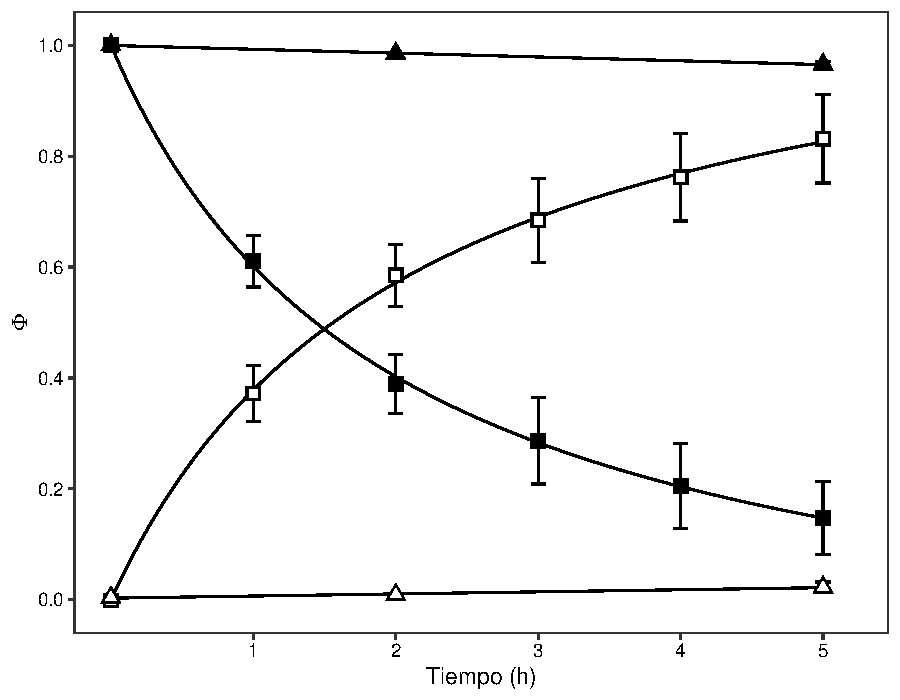
\includegraphics[height=0.388\textwidth]{chap5/figures/K1_pro.pdf}}
               \put(218, 167.5){\large a)}
               \end{picture}}%
    \subbottom{\begin{picture}(230,178)
               \put(0, 0){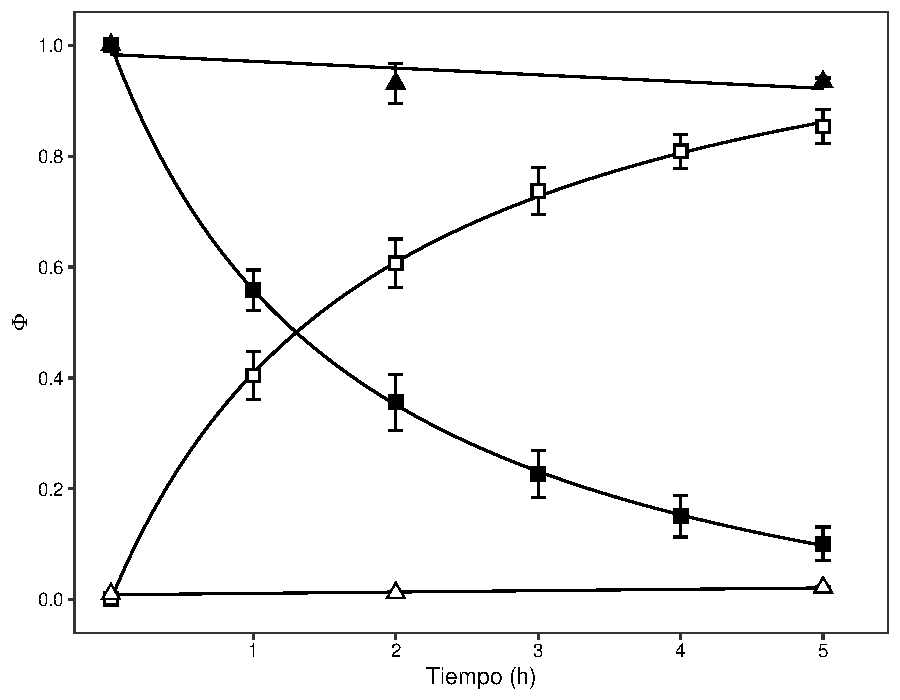
\includegraphics[height=0.388\textwidth, trim = {1.19cm 0 0 0},   clip]{chap5/figures/K9_pro.pdf}}
               \put(199, 167.5){\large b)}
               \end{picture}}
    \caption[Perfiles de transporte de ion litio del sistema bajo optimización.]{Perfiles de transporte de ion litio del punto inicial del simplex (a) y del vértice aceptado como el punto óptimo (b). Fracción de ion litio en la fase de alimentación (\protect\squareblck), fracción de ion litio en la fase de recuperación (\protect\squarewht), sodio en la fase de alimentación (\protect\triangleupblck) y sodio en la fase de recuperación (\protect\triangleupwht). Disolución de alimentación (a): \ce{NH4OH} 0.01~mol~kg\mnn, \ce{Li+} 2~mg~kg\mnn, \ce{Na+} 65~mg~kg\mnn. Disolución de alimentación (b): \ce{NH4OH} 0.016~mol~kg\mnn, \ce{Li+} 2~mg~kg\mnn, \ce{Na+} 65~mg~kg\mnn. Disolución de recuperación (a): HCl 0.07 mol~kg\mnn. Disolución de recuperación (b): HCl 0.1 mol~kg\mnn.}
    \label{fig:simplex2.profiles}
\end{figure}
De un total de 11 experimentos realizados, solo uno de los vértices obtuvo una respuesta mejor que la obtenida en el punto inicial del simplex. La optimización debe detenerse bajo el supuesto de que probablemente el sistema se encuentra muy cerca del punto óptimo y en esta zona el algoritmo de optimización resulta de poca utilidad para encontrar mejores condiciones \citep{simplexbook}. Las condiciones propuestas en el noveno vértice dan lugar a un transporte ligeramente mejor que el que se obtiene con las condiciones de cualquier otro vértice. La respuesta del noveno vértice es significativamente mejor que la del primer vértice, pero la diferencia no es muy grande. La optimización no resultó en una mejora sustancial del proceso de trasporte tal y como se pretendía.

%Los datos de las Tablas \ref{tab:smplx2.1} y \ref{tab:smplx2.2} permiten establecer que el transporte se ve menos favorecido si la masa de la mezcla de extractantes en la membrana es muy pequeña,

Se llevó a cabo el transporte de ion litio bajo las condiciones optimizadas sin incluir sodio en la di\-so\-lu\-ción de alimentación. El perfil de transporte para ion litio se muestra en la Figura \ref{fig:optim10}(a). El coeficiente de permeabilidad de ion litio puede obtenerse de la pendiente de la recta del logaritmo base 10 de la fracción remanente de ion litio en la disolución de alimentación en función del tiempo (Sección \ref{sec:performanceparameters}). La gráfica se muestra en la  Figura \ref{fig:optim10}(b) y el valor obtenido es de (2.13$\pm$0.04)\e{-5}~m~s\mnn. Hay una muy buena relación lineal entre los puntos representados y esto sustenta los supuestos que se hacen para calcular el coeficiente de permeabilidad para ion litio usando este método.
\begin{figure}[H]
    \centering
    \subbottom{\begin{picture}(245,171)
               \put(0, 0){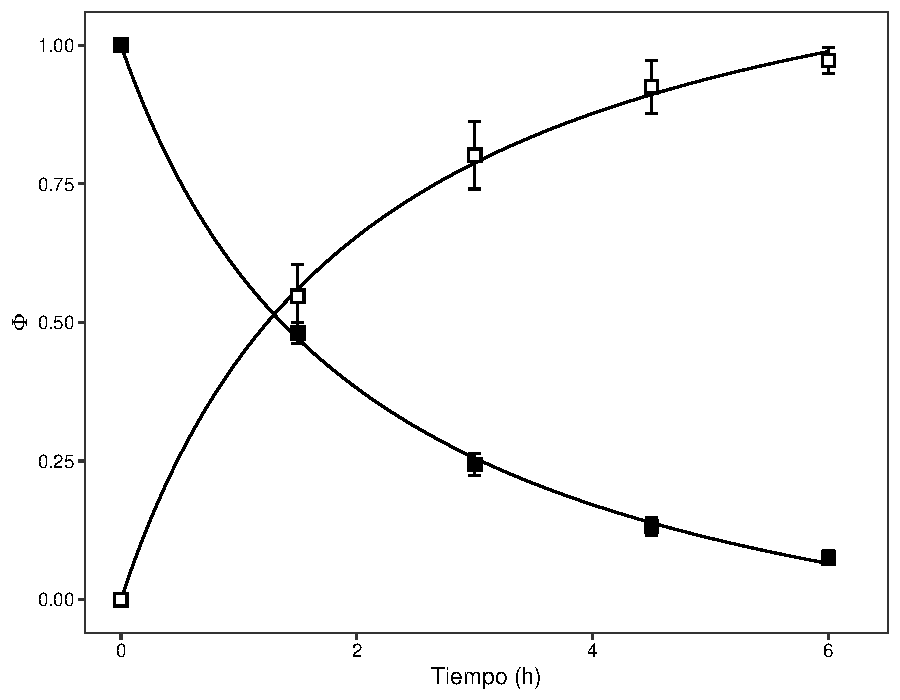
\includegraphics[height=0.383\textwidth]{chap5/figures/K10_pro.pdf}}
               \put(-1, 168){\large a)}
               \end{picture}}%
    \subbottom{\begin{picture}(230,178)
               \put(0, 0){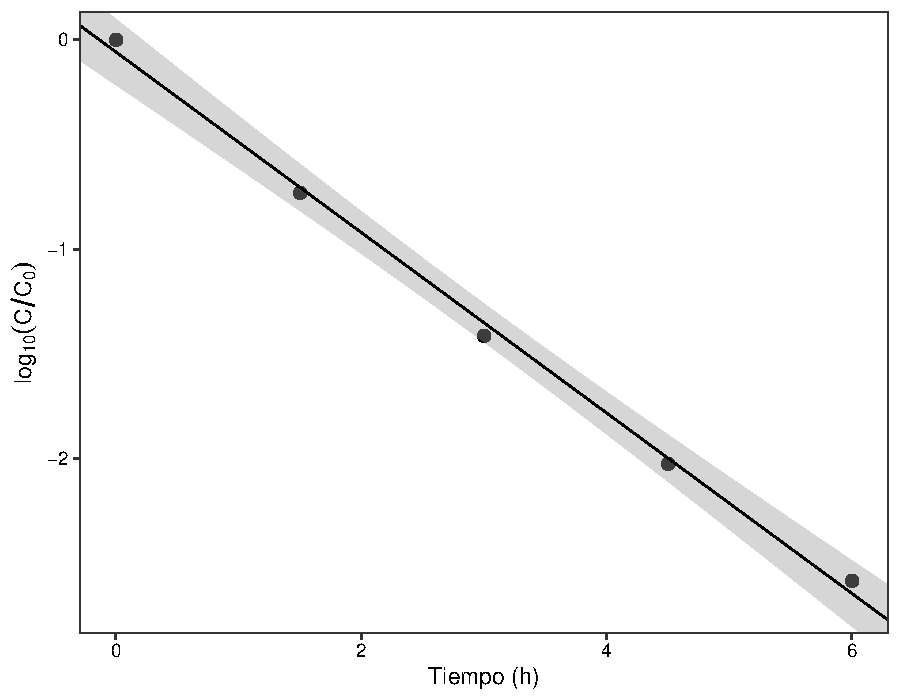
\includegraphics[height=0.383\textwidth, trim = {0 0 0 0},   clip]{chap5/figures/K10_perm.pdf}}
               \put(-1, 168){\large b)}
               \end{picture}}
    \caption[Perfil de transporte de ion litio del sistema optimizado.]{Perfil de transporte de ion litio bajo condiciones optimizadas (a) y gráfico del logaritmo base 10 de la fracción remanente de ion litio en la disolución de alimentación en función del tiempo para el calculo del coeficiente de permeabilidad (b). Fracción de ion litio en la fase de alimentación (\protect\squareblck), fracción de ion litio en la fase de recuperación (\protect\squarewht). La región sombreada corresponde a los intervalos de confianza de la regresión lineal a un nivel de confianza del 95\%. Coeficiente de permeabilidad: (2.13$\pm$0.04)\e{-5}~m~s\mnn. Disolución de alimentación: \ce{NH4OH} 0.016~mol~kg\mnn, \ce{Li+} 2~mg~kg\mnn. Disolución de recuperación: HCl 0.10 mol~kg\mnn.}
    \label{fig:optim10}
\end{figure}

\clearpage\section{Caracterización del sistema optimizado}
\subsection{Selectividad}\label{sec:selecresults}\index{PIM!Selectividad}
Los perfiles de transporte competitivo de ion litio contra sodio, potasio y magnesio en relaciones molares (\ce{Li+}/\ce{M^n+}) 1:1, 1:10 y 1:100 se muestran en la Figura \ref{fig:selectivity1}.

\begin{figure}[H]
    \centering
    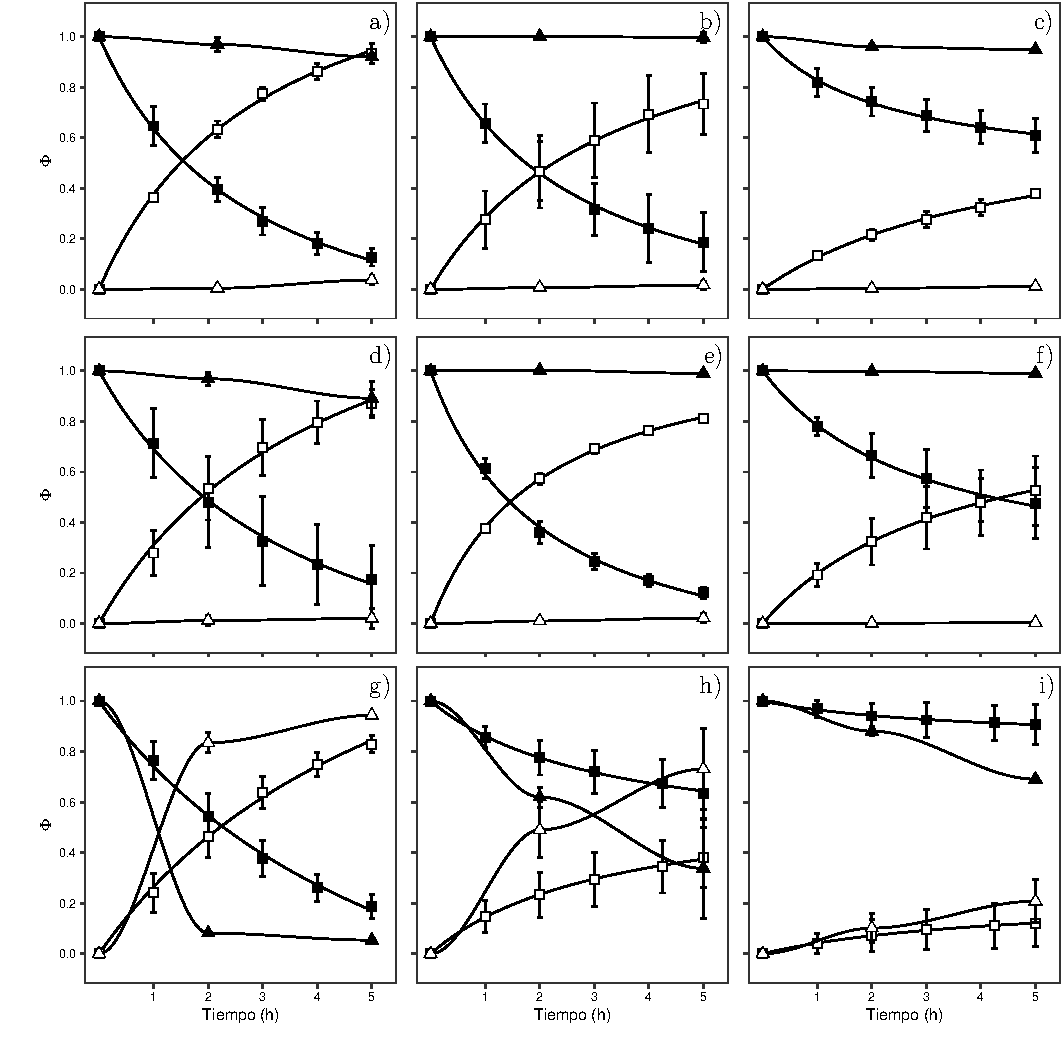
\includegraphics[width=\textwidth]{chap5/figures/thesis-selectividad.pdf}
    \caption[Perfiles de transporte competitivo de ion litio contra sodio, potasio y magnesio.]{Perfiles de transporte de ion litio en presencia de otros cationes interferentes a distintas relaciones molares: sodio 1:1 (a), sodio 1:10 (b), sodio 1:100 (c), potasio 1:1 (d), potasio 1:10 (e), potasio 1:100 (f), magnesio 1:1 (g),  magnesio 1:10 (h) y magnesio 1:100 (i). Ion litio en la fase de alimentación (\protect\squareblck), ion litio en la fase de recuperación (\protect\squarewht), catión interferente en la fase de alimentación (\protect\triangleupblck) y catión interferente en la fase de recuperación (\protect\triangleupwht).}
    \label{fig:selectivity1}
\end{figure}

\clearpage El sistema presenta buena selectividad frente a los cationes alcalinos sodio y potasio. La presencia de estos iones ocasiona una disminución considerable en la permeabilidad de la membrana frente a los iones litio. Este efecto es más marcado cuando las relaciones molares de sodio y de potasio respecto al ion litio son grandes. La fracción transportada de sodio y de potasio se mantiene baja y disminuye con el aumento en su concentración inicial en la disolución de alimentación. Esto se debe a que si la concentración de los iones en la disolución de alimentación es alta, una mayor cantidad neta debe ser transportada para observar un cambio apreciable en las fracciones de cada fase. En otros términos, esto implica que aunque la fracción transportada de sodio y potasio se mantiene baja, una cantidad apreciable de estos iones si es transportada ocupando sitios activos de la membrana y naturalmente, esto disminuye la eficiencia con la que el ion litio es extraído.

Un comportamiento muy diferente lo presenta el catión divalente magnesio que no es excluido por la PIM sino que es transportado incluso con mayor eficiencia que el ion litio. Esto se observa aún cuando su concentración molar es dos órdenes de magnitud mayor a la del ion litio. Varios autores \citep{Liu2020, Zhang2019} han atribuído la falta de selectividad hacia el magnesio por parte de varios de los sistemas destinados a la separación de ion litio al hecho de que los radios iónicos de estos elementos son muy similares: 69 y 72~pm para el ion litio y el magnesio, respectivamente \citep{Marcus1994}. Adicionalmente, el magnesio es un catión divalente y esto hace que en general sea más fuertemente solvatado que el ion litio, que es monovalente \citep{Israelachvili2011}. Se espera que el sistema también presente una pobre selectividad frente al catión calcio.  Los coeficientes de separación son función de la relación molar de cationes presente inicialmente \citep{Chen2018}. Como se observó en la Sección \ref{sec:reprod}, la reproducibilidad de estos valores no es buena.

%\begin{table}[H]
%    \centering
%    \subbottom[]{
%    \begin{tabular}{@{}l c c c @{}}\toprule
%        \multirow{2}{*}{\textbf{Especie}}&\multicolumn{3}{c}{\textbf{Rel. molar}}\\\cline{2-4}
%        & 1:1 & 1:10&1:100\\\midrule
%        Sodio    & 5.4 & 43 & \\
%        Potasio  & 8.0 & 36 & \\
%        Magnesio & >1 & >1& >1\\\bottomrule
%    \end{tabular}
%    }\hspace{5ex}
%    \subbottom[]{
%    \begin{tabular}{@{}l c c c @{}}\toprule
%        \multirow{2}{*}{\textbf{Especie}}&\multicolumn{3}{c}{\textbf{Rel. molar}}\\\cline{2-4}
%        & 1:1 & 1:10&1:100\\\midrule
%        Sodio    & 5.4 & 41 & 33\\
%        Potasio  & 8.0 & 36 & \\
%        Magnesio & >1 & >1& >1\\\bottomrule
%    \end{tabular}
%    }
%    \caption[Factores de separación de ion litio frente a sodio, potasio y magnesio a distintas relaciones molares]{Factores de separación máximos (a) y finales (b) para disoluciones de alimentación con ion litio y sodio, potasio o magnesio a distintas relaciones molares iniciales.}
%    \label{tab:sep-factorlinakmg}
%\end{table}

La aplicación del método a una matriz real (como agua de mar) requiere que el calcio y el magnesio sean retirados del medio antes de intentar la extracción de ion litio. La opción por excelencia es por precipitación selectiva aprovechando la baja solubilidad de distintas sales de estos elementos. Diversos protocolos se han propuesto para la precipitación de estos cationes usando por ejemplo metasilicato de sodio monohidratado \citep{Zhang2019}, ácido oxálico \citep{TRAN2015} o cloruro de potasio con monohidrógenofosfato de sodio en dos etapas \citep{Lai2020}. Las alternativas más comunes involucran precipitación en forma de hidróxidos alcalinizando el medio con hidróxido de sodio \citep{ALAMDARI2008} o hidróxido de amonio \citep{Harvianto2016}. 

La precipitación usando hidróxido de amonio es una idea seductora desde un punto de vista práctico porque no se adicionan cationes alcalinos al medio con lo que el ion litio no se vuelve más difícil de separar. Sin embargo, la precipitación cuantitativa de magnesio bajo estas condiciones no es posible debido a la formación de complejos amoniacales que solubilizan nuevamente al catión \citep{Yamagata2011}. Por otro lado, precipitar el magnesio es relativamente sencillo usando hidróxido de sodio, pero la precipitación cuantitativa de calcio se obtiene a un pH mayor a 13, con lo que la concentración de iones sodio en el medio debería ser aumentada considerablemente. 

\citet{AN2012b} encontraron que la mejor manera de eliminar cationes interferentes de salmueras del Salar de Uyuni (Bolivia) era por medio de una precipitación en dos pasos usando inicialmente carbonato de sodio y posteriormente oxalato de sodio. Este enfoque mitiga el aumento de especies indeseables en la disolución resultante. Con el fin de minimizar el aumento de iones sodio y de remover cuantitativamente los iones calcio y magnesio del agua de mar, se determinó experimentalmente que el magnesio y una fracción importante del calcio pueden retirarse con la adición de hidróxido de sodio a una concentración final de 0.15~mol~kg\mnn. Los iones calcio remanentes son retirados por completo en un paso posterior añadiendo monohidrógenofosfato de amonio a una concentración final de 0.005~mol~kg\mnn. La concentración promedio de iones sodio en agua de mar es de 0.47~mol~kg\mnn \citep{Dickson1994}. El hidróxido de sodio añadido representa un aumento de más del 30\% en la concentración de este catión, pero dado que en agua de mar la relación molar \ce{Na+}/\ce{Li+} es de alrededor de 18000, el panorama no empeora significativamente. Los detalles experimentales de este protocolo se describieron en la Sección \ref{sec:preci}.

\citet{Diaz2019} propusieron una alternativa muy limpia para remover los iones calcio y magnesio presentes en salmueras de ion litio usando electrólisis de membrana en una celda especial. La metodología propuesta permite obtener por separado hidróxido de magnesio e hidróxido de calcio usando hidróxidos provenientes, de la electrólisis reductiva del agua que los contiene. La semireacción que completa la celda electrolítica produce iones hidronio que podrían neutralizar el medio y resolubilizar los hidróxidos recientemente formados pero para evitar esto, el ánodo se encuentra en un compartimiento diferente, separado por una membrana intercambiadora de aniones que no permite su paso hacia el compartimiento donde se encuentra la salmuera bajo tratamiento. Este método no involucra la adición de reactivos precipitantes, sino que estos son generados \textit{in situ}. Los subproductos generados pueden tener valor comercial y la matriz no se hace más compleja (no aumenta la concentración de iones sodio) como consecuencia del proceso. 

\subsection{Capacidad de reuso}\label{sec:reuseres}\index{PIM!estabilidad}
Los perfiles de ion litio remanente en la disolución de alimentación en función del tiempo para los distintos ciclos de extracción de ion litio a partir de una disolución de alimentación ideal se muestran en la Figura \ref{fig:cycles}(a). La fracción transportada de ion litio hacia la disolución de alimentación tras seis horas de cada ciclo se resume en la Figura \ref{fig:cycles}(b).

La eficiencia de la membrana decae casi constantemente tras cada ciclo de reuso. Luego de 10 ciclos de transporte ha perdido cerca del 40\% de la capacidad inicial de la membrana y tiempos mayores pueden ser requeridos para extraer una fracción de ion litio similar a cuando se usa una membrana nueva. La inestabilidad de la membrana puede atribuirse a la alcalinidad de la di\-so\-lu\-ción de alimentación y a la suceptibilidad de las $\beta$-dicetonas (como el LIX-54-100) de lixiviarse desde la PIM bajo estas condiciones \citep{Sugiura1989}.

\begin{figure}[H]
    \centering
    \subbottom{\begin{picture}(242,170)
               \put(0, 0){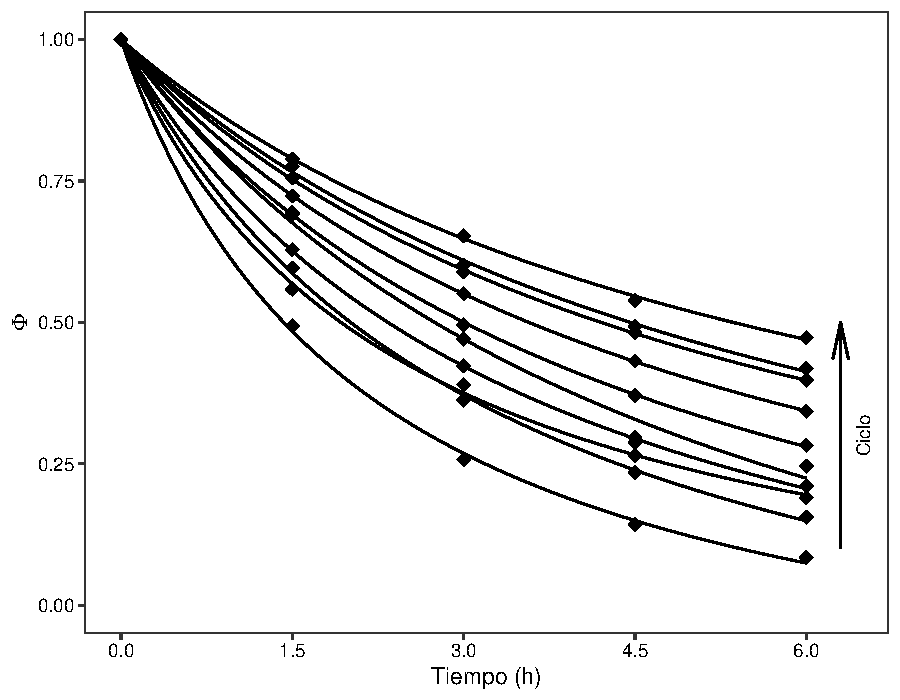
\includegraphics[height=0.388\textwidth]{chap5/figures/reuseprofiles.pdf}}
               \put(219, 168){\large a)}
               \end{picture}}%
    \subbottom{\begin{picture}(230,170)
               \put(0, 0){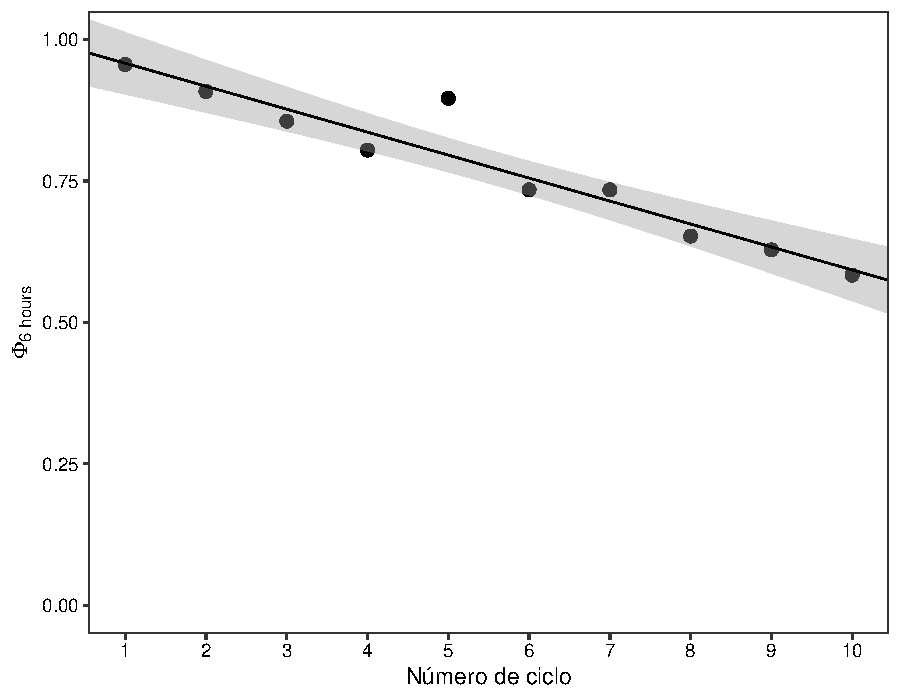
\includegraphics[height=0.388\textwidth, trim = {1.35cm 0 0 0},   clip]{chap5/figures/reusesummary.pdf}}
               \put(197, 168){\large b)}
               \end{picture}}\\
    \caption[Transporte de ion litio en varios ciclos reutilizando la membrana.]{Transporte de ion litio en varios ciclos reutilizando la membrana. (a) Perfiles de transporte desde la disolución de alimentación y (b) fracción transportada de ion litio hacia la disolución de recuperación tras seis horas en cada ciclo. La zona sombreada corresponde al intervalo de confianza de la regresión a un nivel de confianza del 95\%.}
    \label{fig:cycles}
\end{figure}

\subsection{Capacidad de concentración de ion litio}\label{sec:idealconc}
Con los resultados de secciones anteriores se conoció que el sistema es capaz de transportar ion litio en contra de su gradiente de concentración. Esto es posible si su transporte se acopla un contratransporte de iones hidronio. Tras la observación de que la membrana podía ser reutilizada para transportar ion litio se llevó a cabo un experimento similar en el que no se renovó la disolución de recuperación al final de cada ciclo con el propósito de obtener ion litio a una concentración mayor que la disponible inicialmente en la disolución de alimentación. El proceso de transporte se llevó a cabo bajo estas condiciones durante cinco ciclos y el perfil de transporte de ion litio se muestra en la Figura \ref{fig:liconc1}. 

El factor de concentración es de 3.2 luego de cinco ciclos de transporte de ion litio. Esto es equivalente a una eficiencia global de 64\%. Se observa que con cada cambio de la disolución de alimentación disminuye la eficiencia del proceso, como ya se había observado en la Sección \ref{sec:reuseres}. La concentración de ion litio es factible usando la metodología propuesta.

\begin{figure}[H]
    \centering
    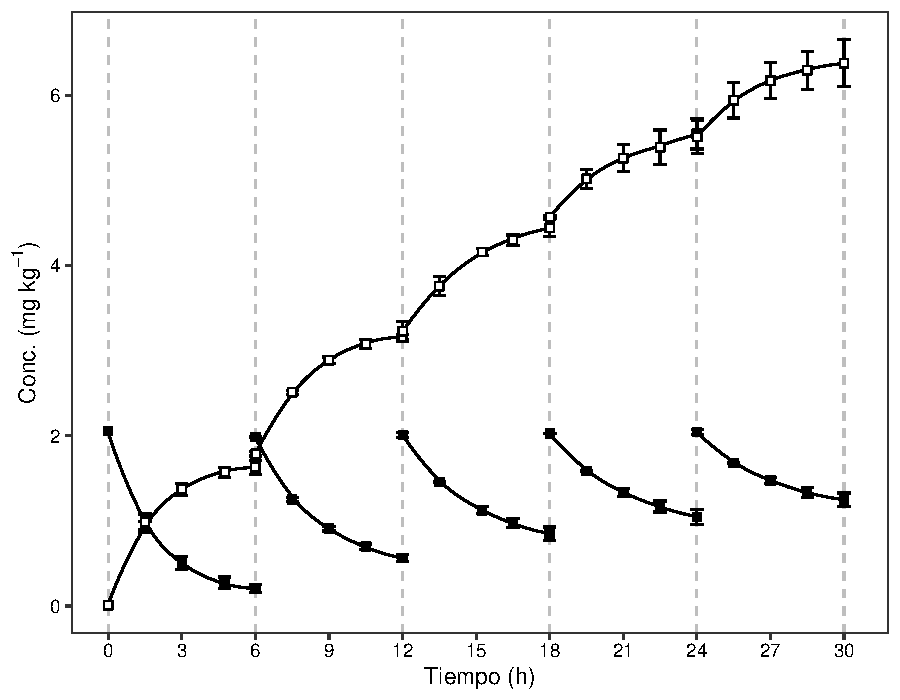
\includegraphics[width = 0.6\textwidth]{chap5/figures/liconc_0.pdf}
    \caption[Concentración de ion litio a partir de una disolución de alimentación ideal.]{Perfil de concentración de ion litio a partir de una disolución de alimentación ideal. Las líneas descontinuas verticales corresponden al inicio o al final de cada ciclo. (\protect\squareblck) ion litio en las disoluciones de alimentación y (\protect\squarewht) ion litio en la disolución de recuperación.}
    \label{fig:liconc1}
\end{figure}


\section{Agua de mar}\label{sec:resultsSSS}\index{Agua de mar}
Como ya se comentó en la Sección \ref{sec:selecresults}, el sistema no es selectivo frente al magnesio y probablemente tampoco lo sea frente al calcio. Estos cationes deben ser retirados del agua de mar antes de intentar extraer el ion litio. La relación molar \ce{Mg^2+}/\ce{Li+} y \ce{Ca^2+}/\ce{Li+} en agua de mar es de 2030:1 y 400:1, respectivamente \citep{Dickson1994}. La concentración final remanente de iones hidroxilo luego del proceso de precipitación por pasos usando hidróxido de sodio y monohidrógenofosfato de amonio se encuentra entre 0.03 y 0.04~mol~kg\mnn. La alcalinidad resultante del medio lo hace adecuado para su uso directo como disolución de alimentación sin la necesidad de añadir reactivos adicionales. 

El perfil de transporte de ion litio, sodio y potasio usando agua de mar sintética simplificada luego de la remoción de iones calcio y magnesio se muestra en la Figura \ref{fig:SSS1}(a). Los factores de separación de ion litio contra sodio y potasio se presentan en la  Figura \ref{fig:SSS1}(b).

El ion litio parece ser transportado en su totalidad hacia la disolución de recuperación tras 4.5 horas de iniciado el proceso. La concentración a la que se encuentra el ion litio en esta matriz es de 0.18~mg~kg\mnn, cerca de diez veces menor a la que contenía la disolución de alimentación con la que el proceso fue optimizado. Para un volumen constante, una menor concentración de ion litio en la disolución de alimentación hace que los cambios de esta magnitud en esta disolución como consecuencia del proceso de transporte, representen una proporción mayor de la especie presente al comienzo del experimento. Debido a esto, la depleción de iones litio de la disolución ocurre en un intervalo de tiempo más corto.  Por otro lado, debe considerarse que la concentración de iones sodio y potasio en el medio es muy alta. Aunque el sistema es muy selectivo frente a estos cationes, se demostró en la Figura \ref{fig:selectivity1} que cuando estas sustancias están a altas concentraciones, su cotransporte afecta de manera importante el transporte de ion litio.

\begin{figure}[H]
  \centering
    \subbottom{\begin{picture}(240,167)
               \put(0, 0){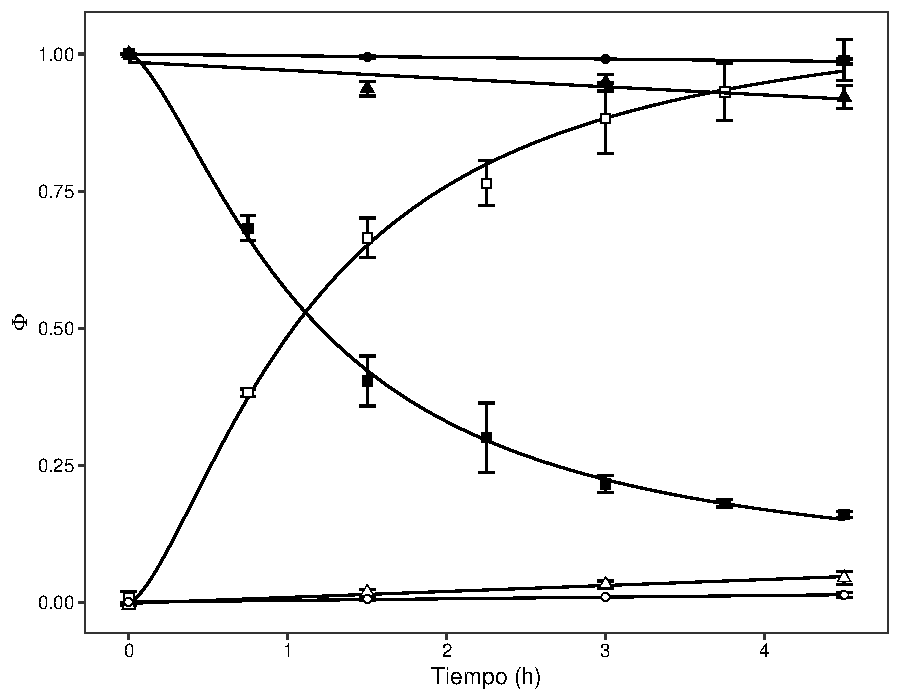
\includegraphics[height=0.37\textwidth, trim = {0cm 0 0 0},   clip]{chap5/figures/sssprof.pdf}}
               \put(-1, 161){\large a)}
               \end{picture}}%
    \subbottom{\begin{picture}(250,167)
               \put(0, 0){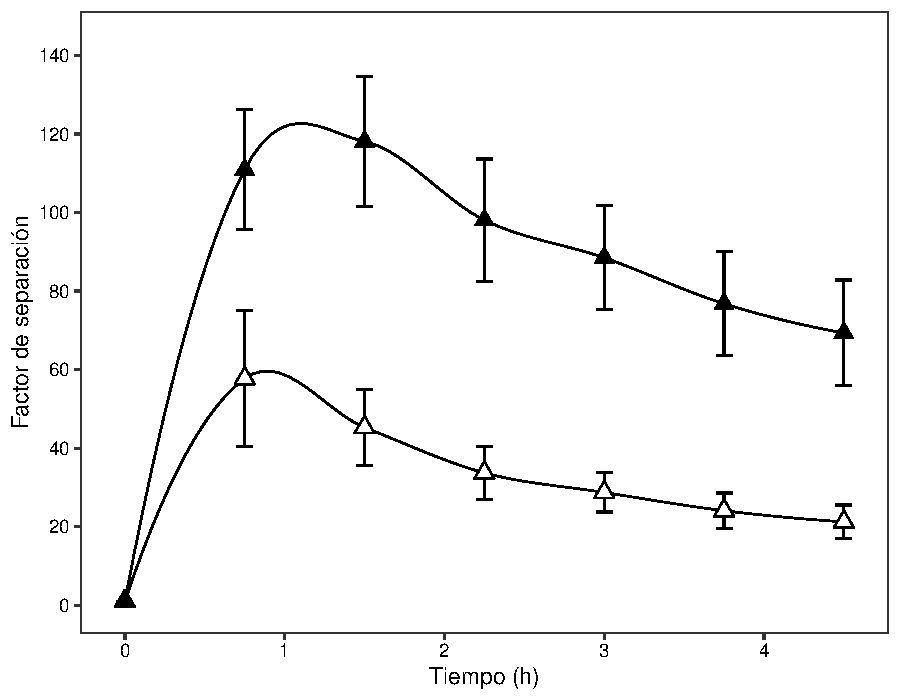
\includegraphics[height=0.37\textwidth, trim = {0cm 0 0 0},   clip]{chap5/figures/sssSep.pdf}}
               \put(-1, 161){\large b)}
               \end{picture}}\\
    \caption[Perfil de transporte y factores de separación usando agua de mar sintética simplificada.]{(a) Perfil de transporte usando agua de mar sintética simplificada: ion litio en la fase de alimentación (\protect\squareblck), ion litio en la fase de recuperación (\protect\squarewht), sodio en la fase de alimentación (\protect\triangleupblck), sodio en la fase de recuperación (\protect\triangleupwht), potasio en la fase de alimentación (\protect\circleblck) y potasio en la fase de recuperación (\protect\circlewht).  (b) factores de separación en función del tiempo: (\protect\triangleupblck) \ce{Li+}/\ce{K+} y (\protect\triangleupwht) \ce{Li+}/\ce{Na+}.}
  \label{fig:SSS1}
\end{figure}


En la Figura \ref{fig:SSS1}(a), la disolución de alimentación parece quedar hacia el final del proceso con un remanente del 15\% del ion litio presente inicialmente. Esto no concuerda con el perfil de transporte de ion litio hacia la disolución de recuperación en  donde aparentemente todo el ion litio es transportado al otro lado de la PIM. Esta posible inconsistencia en el balance de materia del sistema puede justificarse por un efecto matriz de naturaleza traslacional para la cuantificación de ion litio en la matriz de agua de mar. La cuantificación de ion litio se hizo por adición estándar de un punto (ver Anexo \ref{sec:quantification}) y esto mejoró significativamente el balance de materia para ion litio en las disoluciones corrigiendo los efectos matriz rotacionales debidos a los componentes presentes en el agua de mar. Sin embargo, la cuantificación por adición estándar de un solo punto es incapaz de corregir efectos matriz traslacionales \citep{Ellison2008}. Estos efectos matriz difíciles de corregir tienen un efecto más marcado a bajas concentraciones de ion litio. Es probable que en nuestro caso particular, el sesgo introducido cuando la concentración de ion litio es casi nula corresponda a una fracción de 0.15.

Los factores de separación máximos alcanzados frente a sodio y potasio son 118$\pm$16 y 57$\pm$17, respectivamente. Los factores de separación finales frente a sodio y potasio son 69$\pm$13 y 21$\pm$4, respectivamente. El sistema es capaz de selectivamente extraer ion litio de agua de mar.

\subsection{Muestras reales}
\subsubsection{Caracterización}
La concentración de iones litio, sodio, potasio, magnesio y calcio determinadas en las muestras de agua de mar natural recolectadas se muestra en la Tabla \ref{tab:swChar}
\begin{table}[H]
    \centering\footnotesize
    \begin{tabular}{@{}lccccc@{}}\toprule
        \multirow{2}{*}{\textbf{Procedencia}}&[\ce{Li^+}]&[\ce{Na^+}]&[\ce{K^+}]&[\ce{Mg^2+}]&[\ce{Ca^2+}]\\ 
        &(mg~kg\mnn)&(mg~kg\mnn)&(mg~kg\mnn)&(mg~kg\mnn)&(mg~kg\mnn)\\\midrule
        St.\ George Island, Estados Unidos &0.22$\pm$0.03 &~~9870$\pm$110 &359$\pm$22& 1173$\pm$32& 369$\pm$4\\[0.5ex]
        Santa Marta, Colombia &0.23$\pm$0.01 &10732$\pm$134 &401$\pm$10& 1278$\pm$33& 393$\pm$1\\[0.5ex]
        Referencia \citep{Trujillo2016} &0.18&10784&399&1284&415\\\bottomrule
    \end{tabular}
    \caption{Concentración de cationes en las muestras de agua de mar natural.}
    \label{tab:swChar}
\end{table}
La salinidad superficial del agua de mar tiende a ser mayor en inmediaciones a los Trópicos de Cáncer y Capricornio que en la Línea Ecuatorial \citep{Trujillo2016}. Esto se debe a una combinación de factores ambientales que favorecen la evaporación de agua en la zona de los trópicos aumentando la concentración de sales en el agua. La evaporación masiva de agua en la zona Ecuatorial también es un factor importante pero a diferencia de la zona de los Trópicos, la precipitación constante de agua fresca aminora el impacto que esto genera.

Contrario a lo descrito en el párrafo anterior, el agua proveniente de St.\ George Island, Estados Unidos, presenta una concentración menor de cationes respecto al agua muestreada en Santa Marta, Colombia. Esto puede atribuírse a que la isla se encuentra en la Bahía de Apalachicola, donde desemboca el agua dulce del Río Apalachicola. Este es el río más grande del Estado de Florida. El agua del río diluye levemente el agua salada que rodea la isla donde fue tomada la muestra de agua. Por otro lado, la única fuente de `agua dulce' cercana al punto de muestreo en Colombia es el Río Manzanares\footnote{El Río Manzanares sufre de un terrible daño ambiental por descarga de aguas residuales y de varias toneladas de basura al año \citep{Iguaran2019}. Lamentablemente, hace muchos años que sus aguas dejaron de ser \textit{dulces}.}. El caudal del Río Manzanares es pequeño y la Bahía de Santa Marta donde desemboca se encuentra más abierta al mar con lo que la dilución de las sales disueltas en el agua marina es mucho menor.

\subsubsection{Extracción y concentración de ion litio}

Las muestras procedentes de las dos locaciones fueron mezcladas y se removieron los iones calcio y magnesio por precipitación/centrifugación. Se llevaron a cabo cuatro ciclos de extracción de ion litio renovando la disolución de agua de mar en el compartimiento de alimentación. Cada ciclo tuvo una duración de 4.5 horas. 

La concentración de ion litio no es factible usando el sistema propuesto si no se reajusta la concentración de iones hidronio en la disolución de recuperación al final de cada ciclo de transporte. La acidez de la disolución de recuperación disminuye gradualmente y al volverse alcalina esta disolución, el transporte de ion litio no solo se detiene, sino que incluso es transportado de regreso hacia la disolución de alimentación como se muestra a partir del tercer ciclo en la Figura \ref{fig:FAIL}. 

\begin{figure}[H]
    \centering
    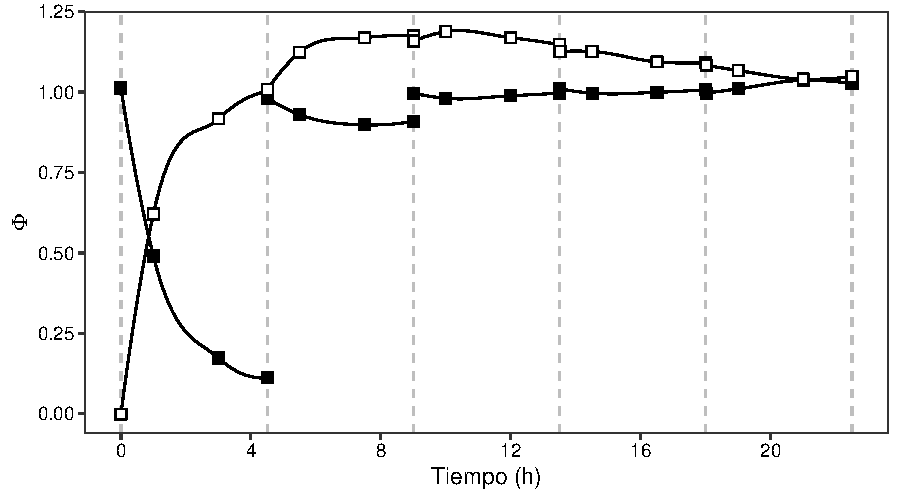
\includegraphics[width=0.65\textwidth, trim = {0cm 0 0 0},   clip]{chap5/figures/LiConcAS-FAIL.pdf}
    \caption[Concentración de ion litio sin reajustar la acidez en la fase de recuperación.]{Perfil de transporte de ion litio cuando se intenta concentrar a partir de agua de mar natural sin reajustar la concentración de iones hidronio en la disolución de recuperación al final de cada ciclo. (\protect\squareblck) ion litio en las disoluciones de alimentación y (\protect\squarewht) ion litio en la disolución de recuperación.}
    \label{fig:FAIL}
\end{figure}

La concentración de iones hidronio en la disolución de recuperación debe ser reajustada al valor original de 0.10~mol~kg\mnn\ al final de cada ciclo de extracción. La disminución en la concentración de iones hidronio en la fase de recuperación no fue importante cuando el ion litio se concentró a partir de una disolución de alimentación ideal. Cuando se usa agua de mar, el flujo de sodio y potasio hacia la disolución de recuperación es significativo a pesar de la buena selectividad del sistema. El flujo de cationes hacia la fase de recuperación conlleva un agotamiento de iones hidronio desde la misma. Si el flujo de cationes es significativo como en este caso, la disolución de recuperación puede volverse alcalina, y al desaparecer el gradiente de iones hidronio el transporte activo de iones litio se detiene. 

Se hizo un nuevo experimento reajustando la concentración de iones hidronio en la fase de recuperación al comienzo de cada ciclo. La concentración de iones litio, sodio, y potasio fue monitoreada en ambas disoluciones durante todo el proceso y los perfiles de transporte obtenidos se muestran en la Figura \ref{fig:liconcSW}. Puede observarse que reajustar la concentración de iones hidronio al final de cada ciclo parece ser suficiente para lograr la concentración de ion litio. Otra alternativa pudo haber sido mantener constante la acidez de esta disolución, por medio de la adición de sustancias amortiguadoras de pH. Esta opción no fue evaluada porque se deseó mantener la matriz de la disolución de alimentación tan simple como fuese posible.

\begin{figure}[htbp]
    \centering
    \subbottom{\begin{picture}(330,145)
               \put(0, 0){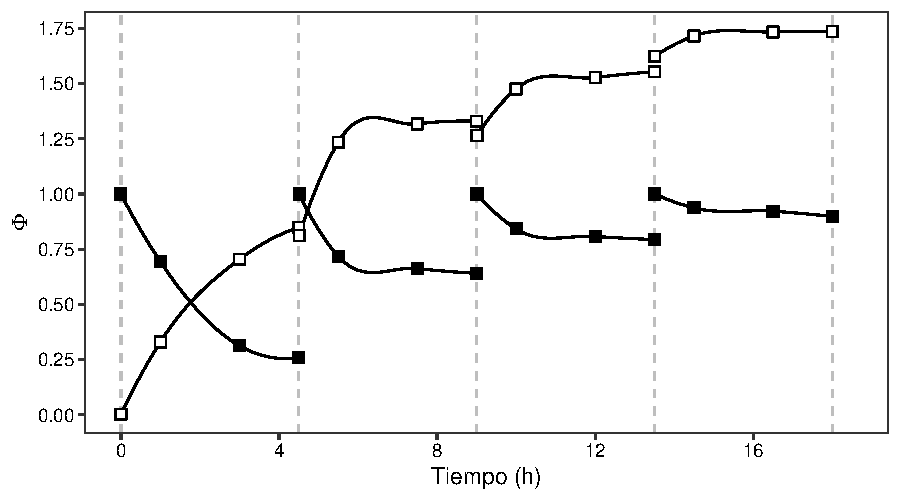
\includegraphics[width=0.65\textwidth, trim = {0cm 0.96cm 0 0},   clip]{chap5/figures/LiConcAS.pdf}}
               \put(-1, 137){\large a)}
               \end{picture}}\\
    \subbottom{\begin{picture}(330,145)
               \put(0, 0){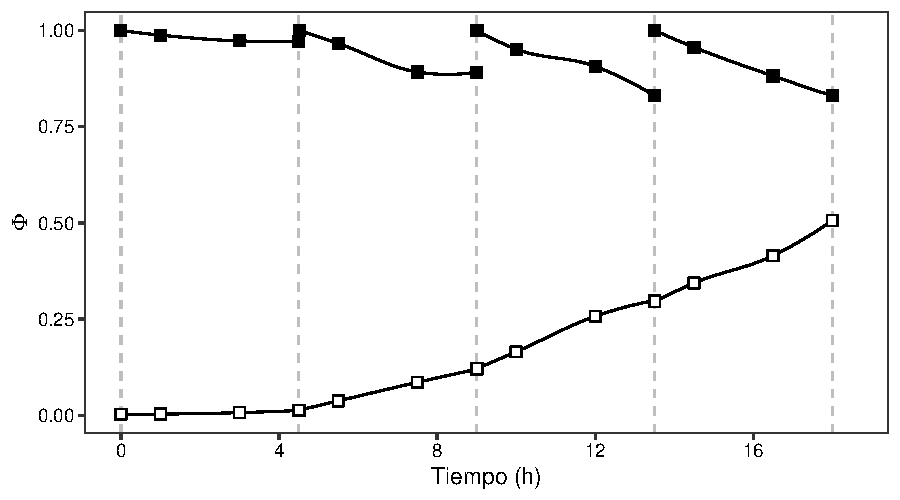
\includegraphics[width=0.65\textwidth, trim = {0cm 0.96cm 0 0},   clip]{chap5/figures/NaConcAS.pdf}}
               \put(-1, 137){\large b)}
               \end{picture}}\\
    \subbottom{\begin{picture}(330,165)
               \put(0, 0){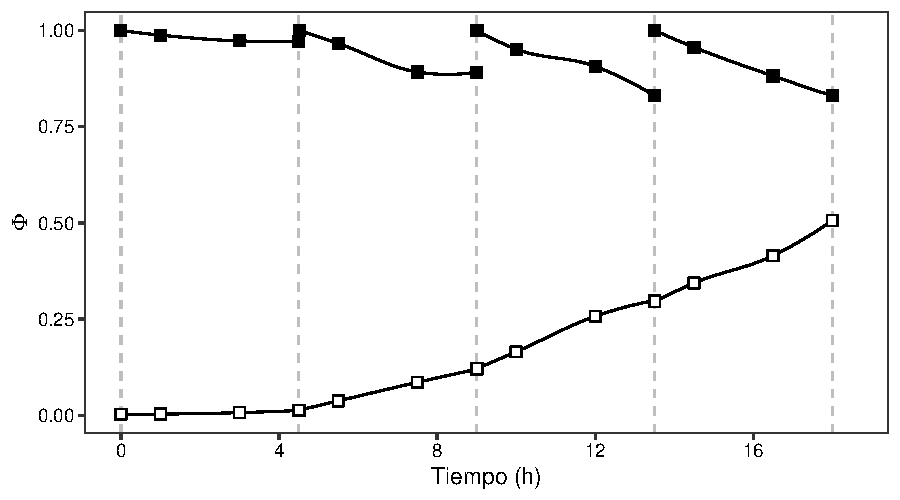
\includegraphics[width=0.65\textwidth, trim = {0cm 0 0 0},   clip]{chap5/figures/KConcAS.pdf}}
               \put(-1, 155){\large c)}
               \end{picture}}
    \caption[Concentración selectiva de ion litio a partir de agua de mar natural.]{Perfil de transporte de ion litio (a), ion sodio (b), e ion potasio (c) a partir de agua de mar natural sin calcio ni magnesio. Las líneas descontinuas verticales corresponden al inicio o al final de cada ciclo. (\protect\squareblck) especie en las disoluciones de alimentación y (\protect\squarewht) especie en la disolución de recuperación.}
    \label{fig:liconcSW}
\end{figure}

La capacidad de la membrana para extraer ion litio se ve deteriorada tras cada ciclo. El perfil de transporte para la concentración de ion litio usando agua de mar (Figura \ref{fig:liconcSW}(a)) difiere significativamente del obtenido cuando se usa una disolución de alimentación sin interferentes (Figura \ref{fig:liconc1}). Al usar una disolución de alimentación ideal, las pérdidas en la eficiencia del transporte disminuyen sutilmente tras cada ciclo y la membrana opera casi al 50\% de su capacidad en el quinto ciclo de concentración. Cuando se usa agua de mar, la eficiencia del sistema en el segundo ciclo es la mitad de la obtenida en el primer ciclo. En el cuarto ciclo la cantidad de ion litio extraído es solo el 13\% del que se extrae en el primer ciclo.

Un comportamiento muy diferente se observa para los cationes interferentes sodio y potasio. La fracción extraída de estos iones al final de cada ciclo es cada vez mayor. Excluyendo los cationes divalentes, la selectividad del sistema es \ce{Li+} $\gg$ \ce{Na+} > \ce{K+} (ver Sección \ref{sec:selecresults}). A partir del segundo ciclo, el orden entre sodio y potasio se invierte y el sistema empieza a extraer potasio con mayor eficiencia que con la que extrae sodio. En el cuarto ciclo la fracción de potasio que es transportada desde la disolución de alimentación es mayor a la de ion litio en casi un 10\%. Esto se presenta a pesar de que el potasio se encuentra en un exceso molar respecto al ion litio de casi 400:1. La selectividad del sistema para extraer ion litio se pierde en este punto y el nuevo orden de afinidad de la membrana pasa a ser \ce{K+} > \ce{Li+} > \ce{Na+}. Los factores de separación de ion litio respecto a sodio y potasio en función del tiempo se muestran en la Figura \ref{fig:SWselec}. Los valores finales de estos factores son 4.9 y 3.4, respectivamente. Los datos del primer ciclo caen en el intervalo de los obtenidos para el mismo experimento cuando la extracción selectiva de ion litio se hizo a partir de la receta de agua de mar sintética simplificada (Figura \ref{fig:SSS1}(b))

\begin{figure}[H]
    \centering
    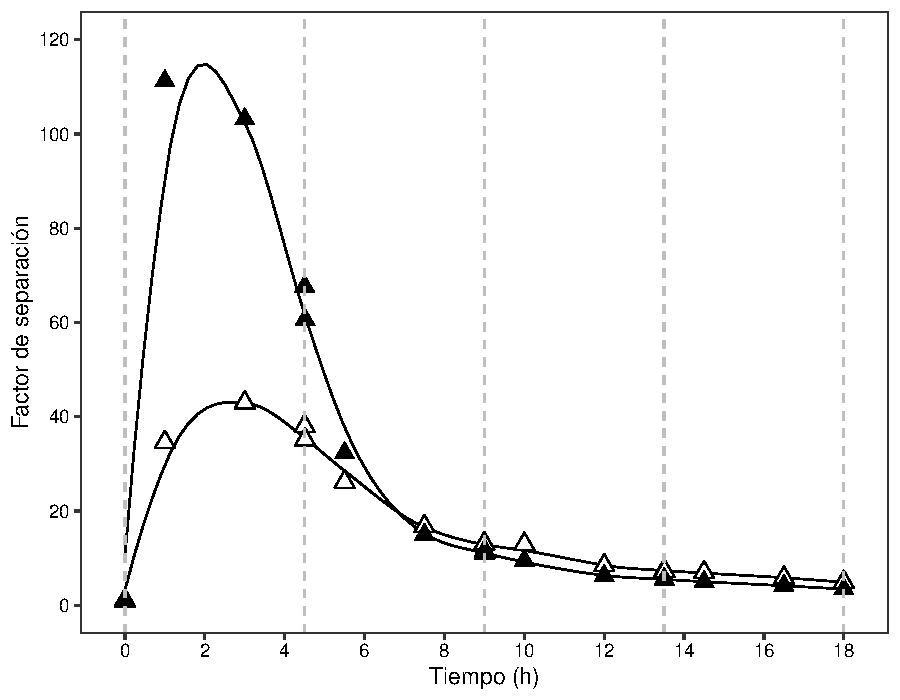
\includegraphics[width=0.6\textwidth, trim = {0cm 0cm 0 0}, clip]{chap5/figures/SW_Sep.pdf}
    \caption[Factor de separación de ion litio frente a sodio y potasio usando agua de mar natural.]{Factores de separación en función del tiempo para la concentración de ion litio usando agua de mar natural: (\protect\triangleupblck) \ce{Li+}/\ce{K+} y (\protect\triangleupwht) \ce{Li+}/\ce{Na+}. Las líneas descontinuas verticales corresponden al inicio o al final de cada ciclo.}
    \label{fig:SWselec}
\end{figure}

El factor de concentración de ion litio en agua de mar es 1.73 luego de cuatro ciclos de extracción. La eficiencia general de este proceso es de al rededor del 43\%, significativamente menor a la reportada en la Sección \ref{sec:idealconc} (64\%).


%\subsection{Resumen}


\clearpage\ChapBib{chap5/results}
    \chapter{Conclusiones y Perspectivas}
\section{Conclusiones}
En el presente estudio se encontraron las condiciones necesarias para extraer ion litio presente a bajas concentraciones en medios acuosos usando una membrana polimérica de inclusión de CTA. Los extractantes mas apropiados fueron LIX-54-100 y Cyanex~923 en una relación molar 2.15:1. La membrana no requiere la adición de un plastificante adicional en la composición de la membrana. El Cyanex~923 tiene la función doble como extractante y plastificante. El sistema presenta buena selectividad frente a los cationes alcalinos sodio y potasio pero los cationes divalentes no son excluidos eficientemente por la membrana. La metodología propuesta fue exitosamente aplicada a la extracción del ion litio presente en muestras de mar. Para esto es necesario retirar por precipitación los cationes divalentes. La propuesta que se hizo fue elevar el pH del medio con hidróxido de sodio, centrifugar la suspensión, añadir una pequeña cantidad de fosfato de amonio a la fase líquida y centrifugar de nuevo para retirar los sólidos suspendidos. El proceso de recobro de ion litio a partir de agua de mar, haciendo uso del protocolo propuesto en este trabajo se esquematiza en la Figura \ref{fig:diagrama}.

{\floatstyle{boxed}
\restylefloat{figure}
\begin{figure}[h]
    \centering
    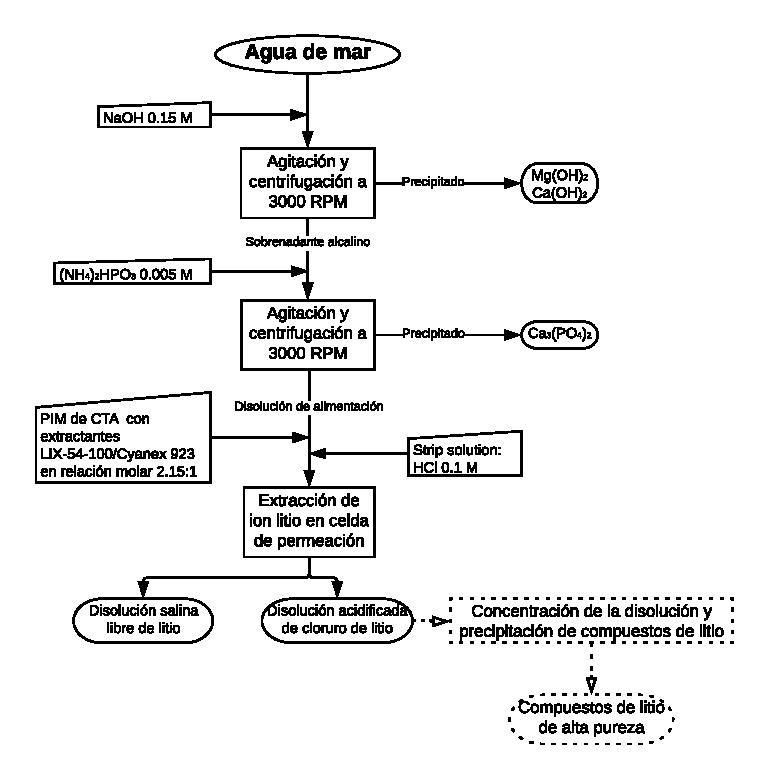
\includegraphics[width = 0.8\textwidth]{chap6/DiagramaProcesoLitioTesis.pdf}
    \caption[Proceso de recobro de ion litio a partir de agua de mar.]{Proceso de recobro de ion litio a partir de agua de mar. La sección del diagrama en línea discontinua son los pasos que no fueron considerados en el presente trabajo.}
    \label{fig:diagrama}
\end{figure}}

La reutilización de las disoluciones de recuperación permiten concentrar al ion litio. Esto fue posible con las disoluciones ideales en las que el ion litio es el único catión metálico presente y con las muestras de agua de mar que contienen excesos molares de iones sodio y potasio de 18000 y 400, respectivamente frente al ion litio. Cuando se concentra el ion litio presente en agua de mar es necesario restaurar el gradiente protónico a través de la membrana al final de cada ciclo para que el transporte pueda ocurrir. No se evaluó la opción de mantener constante el pH de la disolución de recuperación haciendo uso de sustancias amortiguadoras de pH porque se deseó mantener la matriz de las disoluciones tan simple como fuese posible. La selectividad y la eficiencia de la membrana se deterioran con cada ciclo de uso.

La membrana puede ser reutilizada pero tras cada ciclo de uso se pierde eficiencia en el proceso. La membrana tiene una estabilidad regular al conservar solo el 60\% de su capacidad tras diez ciclos de uso de seis horas. El deterioro de la membrana es más marcado cuando se usa agua de mar como disolución de alimentación. Cuando se compara agua de mar sintética simplificada y agua de mar natural el comportamiento del sistema es prácticamente el mismo. 

El coeficiente de permeabilidad de la membrana frente al ion litio, calculado con la Ecuación \ref{eq:coefPerm}, es 2.1 $\times10^{-5}$ m s$^{-1}$. La selectividad del sistema luego de retirar los cationes divalentes del medio es $\ce{Li+}>>\ce{Na+}>\ce{K}$. Los factores de separación en respecto al sodio y al potasio en agua de mar alcanzan valores de hasta 40 y 110, respectivamente. En los factores de separación los valores más altos representan un sistema más selectivo.

Respecto a la disolución de alimentación, se encontró que para que el transporte de ion litio sea posible usando el sistema propuesto, es necesario que la disolución de alimentación sea alcalina. Debido a la naturaleza del algoritmo simplex modificado escogido para optimizar el sistema, no se determinó el valor mínimo de pH necesario para que el transporte de ion litio ocurra, pero este valor debe encontrarse por encima del pKa del LIX-54-100. El pKa del LIX-54-100 debe ser similar al del benzoilacetona (9.61 \citep{Witt2017}). 

Se ha dado cumplimiento al objetivo general y a los objetivos específicos del proyecto. La hipótesis inicial del trabajo ha sido confirmada. El método propuesto podría eventualmente ser adaptado a una escala mayor a la del laboratorio, pero antes de eso deben hacerse consideraciones cuidadosas sobre el posible impacto ambiental y social que puede conllevar la extracción de ion litio a partir de agua de mar. Parece razonable suponer que el impacto a los ecosistemas marinos a causa de la disminución en la concentración de ion litio puede ser pequeño debido al inmenso volumen de agua contenida en los océanos. La extracción del 0.5\% del ion litio presente en los océanos representa una cantidad de litio mucho mayor a la que se ha extraído en toda la historia de la humanidad.

La ecuación empírica propuesta para modelar los perfiles de transporte presenta un excelente ajuste a los datos experimentales y ha resultado de gran ayuda para estudiar la evolución del sistema. De manera similar, el método planteado en la Sección \ref{app:ParedesMethod} para determinar la significancia del efecto de variables explicatorias en un diseño factorial fraccionado ha arrojado resultados muy similares a los que pueden obtenerse con el método gráfico que deriva del dia\-grama de Daniel o con el método de Lenth para determinar la significancia de dichos efectos. Esta metodología presenta algunas similitudes con el algoritmo \ac{NIPALS} que optimiza el número de componentes principales necesarios para describir adecuadamente un conjunto de datos tras la transformación lineal de un \ac{PCA} \citep{Wehrens2011}. Determinar la significancia por este método puede presentar una ventaja sobre el análisis gráfico con los diagramas de Daniel de que no se requiere la asunción \textit{escasez} de efecto.


El paquete \verb|transmem| facilitó significativamente el tratamiento de los datos producidos. Las repre\-sentaciones gráficas que genera son claras, consistentes y estéticas. Tras unos pocos meses luego de su aceptación en el repositorio oficial \ac{CRAN} \citep{transmem}, el paquete ya cuenta con más de 2000 descargas. Se trabajará en su difusión para que sea de utilidad para un mayor número de grupos de investigación que trabajan en el transporte a través de membranas.

\section{Perspectivas}
En el presente trabajo la separación del ion litio no concluyó en la obtención final de un compuesto sólido sino que se obtuvo una disolución en la cual la relación molar de ion litio respecto a otros cationes metálicos es mucho mayor a la originalmente presentada en el agua de mar. La concentración de ion litio en este medio sigue siendo demasiado pequeña como para producir un compuesto de ion litio con un alto nivel de pureza por alguna técnica como precipitación \citep{Nishihama2011}. La obtención de un reactivo con valor comercial a un buen nivel de pureza a partir de la disolución resultante del presente protocolo puede ser el paso a seguir si se desea continuar con el desarrollo del método de extracción propuesto.

Múltiples mejoras pueden ser implementadas al proceso con el fin de proponer una vía más plausible hacia la aplicación del método en el mundo real.

Respecto a los iones divalentes del medio, se ha reportado que el uso de hidróxido de sodio como agente precipitante para la remoción de magnesio presenta conflictos en la posterior separación de fases porque el precipitado que se forma tiene características coloidales \citep{An2012}. El protocolo propuesto en este trabajo involucra hidróxido de sodio e incluye pasos de maduración de precipitado con agitación vigorosa y centrifugación a 3000 \ac{RPM} durante cinco minutos. La separación de fases fue lograda efectivamente y el precipitado formado tiene una excelente consistencia que permite voltear deliberadamente las celdas de centrifugación para recuperar las aguas madres. Considerando las afirmaciones de \citet{An2012}, es probable que este comportamiento tan ideal no sea tan fácil de lograr en escala de planta piloto o planta de producción. 

Una alternativa que valdría la pena probar para remover el magnesio y el calcio puede ser el método de electrólisis de membrana propuesto por \citet{Diaz2019}. Esta puede ser una excelente alternativa para retirar estos cationes del agua de mar sin aumentar la concentración de iones sodio en el medio. Otra ventaja de este procedimiento es que los hidróxidos de calcio y magnesio se obtienen individualmente como precipitados de alto nivel de pureza y podría ser posible su comercialización, con lo que la viabilidad económica del proyecto en conjunto podría ser mayor. Este proceso de electrólisis de membrana puede proveer al medio de la alcalinidad requerida para el proceso de extracción de ion litio usando el protocolo del presente trabajo. La membrana que requiere el método de \citet{Diaz2019} es selectiva a aniones y transporta iones cloruro para mantener la electroneutralidad en ambos compartimientos de la celda. La membrana además evita que los protones generados en el compartimiento anódico neutralicen la disolución y se residuelvan los hidróxidos que se están retirando. La membrana selectiva a aniones podría ser innecesaria si se usa un ánodo de plata, sobre el cual podría depositarse cloruro de plata a medida que en el cátodo se presenta la evolución de hidrógeno con la respectiva formación de iones hidroxilo como consecuencia de la reducción del agua. El electrodo de plata queda recubierto de cloruro de plata con lo que en algún momento quedaría inutilizable, pero puede ser regenerado a través de la inversión del potencial aplicado (en una disolución salina) para reducir la plata del cloruro de plata.

Por otro lado, para concentrar el licor de ion litio que se obtiene como disolución de recuperación, puede probarse la ósmosis directa usando membranas de \ac{CTA} que ha sido aplicada por \citet{Li2018} para retirar parte importante del disolvente y aumentar la concentración de ion litio en una salmuera de un lago salado. Esta técnica no produce subproductos indeseables y el gasto energético es mínimo dado que contrario a la ósmosis inversa, la fuerza motriz en este caso es el potencial osmótico propio de las disoluciones. Como disolución de arrastre podría usarse el agua de mar que ya fue utilizada en el proceso de extracción de ion litio. 

Durante los experimentos de concentración de ion litio de agua de mar, la celda de transporte se dejó en laboratorio durante una semana y se observó una disminución progresiva del volumen de la disolución de recuperación con un aumento de similar proporción en el volumen de la disolución de alimentación. No se determinó si el ion litio presente en la disolución de recuperación había aumentado su concentración, pero es probable que un proceso de ósmosis directa haya tenido lugar ya que membranas de \ac{CTA} han demostrado ser de utilidad para este tipo de procedimientos \citep{Li2018}.

Un trabajo futuro podría incorporar un potencial eléctrico como fuerza motriz para el transporte de ion litio a través de la \ac{PIM}. Los métodos electroquímicos acoplados a membranas selectivas son actualmente muy estudiados y han sido exitosamente aplicados a la extracción de ion litio a partir de agua de mar \citep{LIU2019}. Adaptar este enfoque a la PIM propuesta en esta tesis podría generar electrodialisis selectiva de membrana. Esta combinación de técnicas ha sido empleada en distintas ocasiones para mejorar el transporte de diversas especies a través de PIMs \citep{Kaya2016, See2013} pero aún no ha sido aplicada al transporte de ion litio a través de estas membranas.

El impacto ambiental de la fabricación de las membranas podría disminuirse si se evalúa la preparación de las PIMs usando el proceso libre de disolventes reportado por \citet{Vera2019}. Al no usar disolventes orgánicos clorados, la emisión de vapores perjudiciales para la atmósfera es anulada. Esto requiere que se caractericen térmicamente los extractantes y que se reemplace el polímero base por uno con punto de fusión más bajo \citet{Vera2019}.

La estabilidad y la permeabilidad de la membrana frente a iones litio podría incrementarse significativamente si se incursiona en el uso de polímeros base entrecruzables para producir PIMs de \textit{nueva generación} \citep{OBRYAN2017}.

Finalmente, un nuevo trabajo de tesis relacionado con la extracción de ion litio usando PIMs podría involucrar el uso de líquidos iónicos similares a los reportados por \citet{ZANTE2019} o por \citet{Shi2020}. El desempeño de esta nueva membrana puede ser comparado con el de las membranas reportadas en el presente trabajo. Las perspectivas propuestas en párrafos anteriores podrían ser probadas en la membrana que resulte más apta tras hacer la comparación. El trabajo interdisciplinar involucraría la síntesis de los líquidos iónicos y el estudio del sistema electroquímico para la extracción.
\clearpage
\ChapBib{chap6/conclusions}
    \appendix
        \chapter{Artículo Aceptado en Revista Desalination}\label{sec:article}
Los resultados de la presente tesis fueron recopilados en un artículo de investigación que fue aceptado para publicación en la revista de primer cuartil \textit{Desalination} de la editorial Elsevier. La revista \textit{Desalination} publica artículos relacionados con ciencia y tecnología de desalinización y purificación de agua incluyendo entre sus tópicos, la recuperación de recursos a partir de salmueras.

El manuscrito se incluye en las siguientes páginas en versión de \textit{prueba sin corregir}.
\includeArticle{1}
\includeArticle{2}
\includeArticle{3}
\includeArticle{4}
\includeArticle{5}
\includeArticle{6}
\includeArticle{7}
\includeArticle{8}
\includeArticle{9}
\includeArticle{10}
        \chapter{Cuantificación de Cationes Metálicos}\label{sec:quantification}
\vspace{-1cm}%\enlargethispage{\baselineskip}
Para cuantificar los cationes metálicos se empleó un espectrómetro de absorción atómica Perkin-Elmer 3100 siguiendo las especificaciones recomendadas por el fabricante \citep{perkin}. El instrumento puede configurarse para trabajar en modo \ac{FAAS} y en modo \ac{FAES}. Las condiciones instrumentales empleadas para cada ele\-mento se encuentran en la Tabla~\ref{tab:FAASconditions}. En todos los casos se usó una llama oxidante (azul) de aire/acetileno en relación de volumen~2:1. 

\newcolumntype{P}[1]{>{\centering\arraybackslash}p{#1}}
\begin{table}[H]
    \centering\footnotesize
    \begin{tabular}{@{}p{1.5cm}P{1cm}P{2.6cm}P{1cm}P{1cm}P{1cm}l@{}}\toprule
        \multirow{2}{*}{\textbf{Elemento}}&$\lambda$ &\textbf{RT} &\textbf{AR} &\textbf{TI} &\textbf{ICL}&\textbf{Modelo}\\
        &(nm)&(mg~kg$^{-1}$)&(nm)&(s)&(mA)\\\midrule
        Litio   &670.8 &5 - 250 (\e{-3}) & 0.7& 0.3&(FAES) & Lineal\\
                &      &0.05 - 2.00 & 0.7& 0.5&8 & Lineal\\
        Sodio   &589.0 &0.10 - 8.00 & 0.4& 0.5&(FAES) & Cuadrático\\
        Potasio &776.5 &0.20 - 2.30 & 0.7& 0.5&(FAES) & Cuadrático\\
        Magnesio&285.2 &0.23 - 1.16 & 0.7& 0.5&verificar \\
        Calcio  &427.7 &1.00 - 5.15 & 0.7& 0.5&verificar \\\bottomrule
        \multicolumn{7}{@{}l@{}}{\tiny\textbf{RT:} Rango de trabajo; \textbf{AR:} Ancho de rendija; \textbf{TI:} Tiempo de integración; \textbf{ICL:} Intensidad de corriente de la lámpara}
    \end{tabular}
    \caption{Condiciones instrumentales para la determinación de elementos por FAAS y FAES.}
    \label{tab:FAASconditions}
\end{table}

\vspace{-0.7cm}En el presente trabajo fue necesario trabajar con muestras altamente salinas como agua de mar (más de 35~g~kg\mnn\ de sólidos disueltos). Estas muestras no podían ser diluidas para determinar la concentración del litio que se encuentra a un muy bajo nivel. Tras la lectura de tales disoluciones el efecto memoria del instrumento era evidente y recalcitrante. El amarillo color característico de la llama con sodio no desaparecía fácilmente si se esperaba a lavar la cámara de nebulización con protocolos normales como aspirar agua desionizada o ácido diluido por un par de minutos. Para minimizar el consumo de combustible y el tiempo requerido para eliminar el efecto memoria se propuso cerrar el flujo de acetileno y subir al máximo el flujo de aire mientras se aspira por el capilar una mezcla de ácido nítrico 2\% con ácido clorhídrico 3\% en agua desionizada. La mezcla de ácidos en combinación con el alto flujo de aire disminuyó considerablemente el tiempo requerido para limpiar la cámara y dejar el equipo listo para determinar el siguiente elemento.


\section{Determinación de ion litio}
La cuantificación de ion litio se abordó desde diversos enfoques dependiendo de las características del experimento realizado. Se usó curva de calibración por patrón externo con concordancia de matriz para experimentos en los que las matrices de las disoluciones de alimentación y de recuperación no variaron significativamente durante el proceso de transporte. Si durante el experimento una de las disoluciones varía sistemáticamente de manera medible en un solo parámetro que se conoce afecta la respuesta del método (e.g. aumento paulatino de iones sodio en la fase de recuperación), la técnica de cuantificación aplicada fue regresión plana. Finalmente, en experimentos que involucraron matrices complejas como agua de mar (sintética o natural), se cuantificó el ion litio haciendo uso de la adición estándar de un solo punto.

La disolución concentrada de ion litio que fue utilizada como patrón inicial fue preparada con carbonato de litio seco que se disolvió en un ligero exceso de ácido clorhídrico. Para la cuantificación por estándar externo con concordancia de matriz o con regresión multiparamétrica se utilizó \ac{FAAS} y para la cuantificación por adición estándar de un solo punto se utilizó \ac{FAES} que es más sensible a bajas concentraciones.

\subsection{Concordancia de matriz}\label{sec:liexternal}
Las curvas de calibración por \ac{FAAS} para ion litio en ácido clorhídrico 0.1~mol~kg\mnn\ (fase de recuperación) y en hidróxido de sodio 0.1~mol~kg\mnn\ (fase de alimentación) se muestran en la Figura \ref{fig:LitCurve}. Los estándares de calibración fueron preparados por dilución gravimétrica de la disolución concentrada.

\begin{figure}[H]
    \centering
    \subbottom{\begin{picture}(242,170)
               \put(0, 0){\includegraphics[height=0.388\textwidth]{App/images/LiCurves.pdf}}
               \put(24, 168){\large a)}
               \end{picture}}%
    \subbottom{\begin{picture}(230,170)
               \put(0, 0){\includegraphics[height=0.388\textwidth, trim={1.3cm 0 0 0}, clip, page=2]               {App/images/LiCurves.pdf}}
               \put(5, 168){\large b)}
               \end{picture}}\\
    \caption[Curvas de calibración para ion litio en medio ácido y en medio alcalino.]{Curvas de calibración para ion litio en ácido clorhídrico 0.1~mol~kg\mnn\ (a) y en hidróxido de sodio 0.1~mol~kg\mnn\ (b) por FAAS. Se incluyen las curvas de regresión lineal donde la zona sombreada gris es el intervalo de confianza para la regresión con una significancia del 99\%.}
    \label{fig:LitCurve}
\end{figure}
\clearpage Las ecuaciones que describen las curvas de calibración para la fase de recuperación y de alimentación se muestran en las Ecuaciones \ref{eq:litRec} y \ref{eq:litAli}.
\begin{equation}\label{eq:litRec}
    Abs_{670.8~nm}=(0.000\pm0.001)+(0.156\pm0.002) C_{\ce{Li^+}}
\end{equation}
\begin{equation}\label{eq:litAli}
    Abs_{670.8~nm}=(0.000\pm0.001)+(0.183\pm0.002) C_{\ce{Li^+}}
\end{equation}
donde la concentración de ion litio ($C_{\ce{Li^+}}$) se encuentra en mg~kg\mnn. Hay diferencias estadísticamente significativas entre las pendientes de las curvas indicando que hay un efecto matriz presente que debe ser tenido en cuenta.


\subsection{Regresión multiparamétrica (plana)}\label{sec:planar1}
La presencia de iones sodio magnifica la señal de absorbancia de litio. Una regresión bivariada que considere la concentración de ion sodio entre las variables explicatorias puede mitigar el sesgo que se observa a causa de este factor. La regresión plana se hizo para considerar el efecto de cantidades variables de sodio que es transportado a la fase de recuperación durante el proceso de transporte. Un plano de regresión para valores de concentración de ion litio entre 0.05 y 2.00~mg~kg\mnn\ en presencia de cantidades variables de sodio (entre 0 y 250~mg~kg\mnn) se muestra en la Figura \ref{fig:planarLit}. Los estándares de calibración fueron preparados gravimétricamente a partir de la dilución de disoluciones concentradas de cloruro de litio y de sodio.

\begin{figure}[H]
    \centering
    \includegraphics[width=0.5\textwidth, trim={3cm 2.5cm 2.05cm 2.3cm}, clip]{App/images/LiPlane.pdf}
    \caption{Plano de calibración para ion litio considerando la concentración de sodio.}
    \label{fig:planarLit}
\end{figure}
\clearpage La relación con el ion litio es similar a la presentada en las curvas de la Figura \ref{fig:LitCurve}. Puede observarse una inclinación ligera en el plano a medida que aumenta la concentración de sodio. La ecuación del plano es:
\begin{equation}\label{eq:litPlan}
    Abs_{670.8~nm}=(-0.002\pm0.001)+(0.1588\pm0.0008) C_{\ce{Li^+}}+(3.2\pm0.7)\e{-5} C_{\ce{Na^+}}
\end{equation}
donde la concentración de las especies está en mg~kg\mnn. 

El intercepto del plano sigue sin ser estadísticamente diferente de cero. La dependencia de la señal frente a la concentración de ion litio y de sodio sí es estadísticamente significativa. La sensibilidad del método hacia el ion litio es cuatro órdenes de magnitud mayor que hacia el sodio. Sin embargo, la concentración de sodio en la disolución de recuperación puede aumentar mucho más rápido que la del ion litio con lo que el efecto llegaría a ser importante y la regresión multiparamétrica podría ser de utilidad. Para calcular la concentración de ion litio a partir de una medición de absorbancia empleando el plano de regresión es necesario conocer (medir) la concentración de sodio en las disoluciones. 

\subsection{Adición estándar de un solo punto}
La disolución de recuperación sufre cambios drásticos cuando se extrae ion litio desde agua de mar sintética o natural. La mejor manera de contrarrestar el efecto matriz en la cuantificación de ion litio como consecuencia de estos cambios es por medio del método de adiciones estándar. La cuantificación de especies por adiciones estándar requiere que la señal del mesurando sea medida en conjunto con otras disoluciones enriquecidas con el mismo analito a determinar a un nivel conocido. La estrategia es eficiente para corregir los efectos matriz rotacionales cuyo efecto es un cambio en la sensibilidad del método (i.e.\ la pendiente de la curva de calibración) debido a la presencia de otros componentes.

Las adición estándar asume que una respuesta nula es producida por una muestra en la que la concentración de analito es también nula. La manera más común de obtener un resultado implica graficar la señal medida contra la concentración de analito adicionada. Debe incluirse el dato de la señal de la muestra sin enriquecer que corresponde a la señal de la muestra original. La extrapolación de los datos obtenidos hasta su intercepto con el eje de las abscisas corresponde al inverso aditivo de la concentración del analito en la muestra original.

Este método presenta la desventaja de que consume un mayor tiempo en la preparación de las muestras pues es equivalente a preparar una curva de calibración por cada muestra. Sin embargo, se ha demostrado que una cuantificación con buenas cualidades metrológicas puede obtenerse con la adición de un solo punto de muestra enriquecida \citep{Ellison2008}. Se recomienda que la muestra original y la muestra enriquecida sean diluidas de igual manera para que los constituyentes de la matriz original se encuentren a la misma concentración en ambas disoluciones. Sin embargo, cuando el factor de dilución que sufre la muestra enriquecida como consecuencia de la masa de disolución estándar adicionada es pequeño, este efecto es pequeño y puede ser despreciado.

En términos prácticos se divide la muestra disponible en dos viales, de los cuales en uno debe medirse la masa de disolución que ha sido agregada. El vial que contiene la masa conocida de disolución ($m_0$, cerca de 600~mg en nuestro caso) es adicionado con una masa conocida ($m_s$, cerca de 60~mg) de disolución estándar de ion litio con concentración conocida ($C_{\ce{Li+}}^{stock}$, 530~$\mu$g~kg\mnn). Se debe medir la señal de emisión de litio en la muestra original ($Em_{670.8~nm}^0$) y de la muestra enriquecida que debe ser cuidadosamente homogeneizada antes de la medición ($Em_{670.8~nm}^s$). La ecuación que se emplea en para conocer la concentración original de ion litio en la muestra ($C_{\ce{Li+}}^0$) es:
\begin{equation}
    C_{\ce{Li+}}^0 = C_{\ce{Li+}}^{stock} \cdot\frac{Em_{670.8~nm}^0  \big(\frac{m_s}{m_s+m_0}\big)} {Em_{670.8~nm}^s-Em_{670.8~nm}^0\big(\frac{m_0}{m_s+m_0}\big)}
\end{equation}
Es indispensable que ambas mediciones de emisión atómica caigan en el rango lineal del método. Para esto, el máximo de emisión en el instrumento se configuró con el estándar que es añadido para enriquecer las muestras ($\sim500~\mu$g~kg\mnn). Esto proporciona un excelente rango lineal entre 5 y 270~$\mu$g~kg\mnn\ como se muestra en la Figura \ref{fig:Rangolineal}. Ninguna muestra original o enriquecida debe tener una emisión mayor a la del límite superior del rango lineal y si esto se presenta, la muestra debe ser diluida gravimétricamente.

\begin{figure}[H]
    \centering
    \includegraphics[height=0.388\textwidth]{App/images/LiRange.pdf}
    \caption[Rango lineal de la emisión de litio a bajas concentraciones]{Rango lineal de la emisión de litio a bajas concentraciones. Se incluye la curva de regresión lineal donde la zona sombreada gris es el intervalo de confianza para la regresión con una significancia del 99\%.}
    \label{fig:Rangolineal}
\end{figure}

\section{Determinación de sodio y potasio}
Las especies sodio y potasio fueron cuantificadas por \ac{FAES} usando curvas de calibración por patrón externo que se ajustaron a polinomios de grado 2. Los estándares de calibración se prepararon por dilución sucesiva de disoluciones concentradas de estos cationes que fueron preparadas a partir de sus respectivas sales de cloruro secas. Para disminuir el sesgo en las determinaciones, los estándares de calibración se prepararon en matrices similares a aquellas de las muestras considerando sus respectivos factores de dilución.

La baja energía de ionización de los metales alcalinos los hace susceptibles de perder electrones en el proceso de atomización y sus especies iónicas no presentan las mismas líneas de absorción o emisión de las especies atómicas. Esto ocasiona una disminución en la señal de estos elementos que se conoce como \textit{interferencia no espectral por ionización}. La mejor manera de corregir este tipo de interferencia es con la adición de un \textit{amortiguador de ionización} que es una especie fácilmente ionizable (generalmente metales alcalinos) que debe encontrarse a concentraciones altas. Los amortiguadores de ionización más utilizados son sales cloruro de potasio, cesio, litio, y lantano a una concentración final en disolución de 0.1\%. 

Ejemplos de las curvas de calibración para sodio y potasio se muestran en la Figura \ref{fig:SodPot}. Las curvas fueron obtenidas usando cloruro de potasio para la determinación de sodio y cloruro de litio para la determinación de potasio (amortiguadores de ionización). En ambos casos se usó el estándar de más alta concentración para configurar el máximo de emisión respecto al cual son medidos los demás estándares y las muestras.

Las curvas obtenidas presentan un excelente ajuste y el intervalo de confianza a un nivel de significancia de 0.99 es muy delgado. Se probó el desempeño de los cloruros de lantano y de cesio como supresores de ionización pero dieron lugar a curvas de calibración con muy mala correlación por lo que no fueron incluidas. 

\begin{figure}[H]
    \centering
    \subbottom{\begin{picture}(242,170)
               \put(0, 0){\includegraphics[height=0.388\textwidth]{App/images/NatKalCurves.pdf}}
               \put(24, 168){\large a)}
               \end{picture}}%
    \subbottom{\begin{picture}(230,170)
               \put(0, 0){\includegraphics[height=0.388\textwidth, trim={1.35cm 0 0 0}, clip, page=2]               {App/images/NatKalCurves.pdf}}
               \put(5, 168){\large b)}
               \end{picture}}\\
    \caption[Curvas de calibración para sodio y potasio por FAES.]{Curvas de calibración para sodio en cloruro de potasio 0.1\% (a) y potasio en cloruro de litio 0.1\% (b) por FAES. Se incluyen las curvas de regresión cuadrática donde la zona sombreada gris es el intervalo de confianza para la regresión con una significancia del 99\%.}
    \label{fig:SodPot}
\end{figure}

Las respectivas ecuaciones que describen las curvas de calibración se muestran en las Ecuaciones \ref{Eq:Nat} y \ref{Eq:Pot}. Los interceptos de las curvas con el eje de las ordenadas no son estadísticamente significativos.

\vspace{-0.8cm}
\begin{equation}\label{Eq:Nat}
    Em_{589.0~nm}=(0.000\pm0.002)+(0.166\pm0.002) C_{\ce{Na^+}} - (0.0049\pm0.0003) C_{\ce{Na^+}}^2
\end{equation}
\begin{equation}\label{Eq:Pot}
    Em_{776.5~nm}=(0.000\pm0.002)+(0.496\pm0.005) C_{\ce{K^+}} - (0.047\pm0.002) C_{\ce{K^+}}^2
\end{equation}
donde la concentración de las especies ($C_{\ce{M^+}}$) se encuentra en mg~kg\mnn. Los parámetros de las ecuaciones de regresión varían ligeramente en función de la temperatura de los estándares, la altura del quemador, el flujo del nebulizador y el instrumento que se utilice.

\section{Determinación de magnesio y calcio}
Las especies magnesio y calcio fueron cuantificadas por \ac{FAAS} usando curvas de calibración por patrón externo que presentaron un buen ajuste a una función cuadrática y lineal, respectivamente. Los estándares de calibración se prepararon por dilución sucesiva de di\-so\-luciones concentradas de estos cationes que fueron preparadas a partir de sus respectivas sales de carbonato secas disueltas en un ligero exceso de ácido clorhídrico.

Estas especies forman compuestos refractarios cuando hay fosfatos en el medio. La formación de estos compuestos refractarios impide la atomización necesaria para que ocurra la absorción atómica y conduce a una disminución en la señal de estos elementos. Solucionar esta \textit{interferencia química} es sencillo con la adición de cloruro de lantano al 0.1\%. El lantano forma compuestos refractarios más estables que desplazan el equilibrio de formación de estos compuestos con calcio y magnesio y los liberan para que puedan ser cuantificados tranquilamente. El cloruro de lantano en disolución que fue adicionado a las muestras y a los estándares se preparó disolviendo óxido de lantano en ácido clorhídrico 1:1 y completando a la masa deseada con agua desionizada.

Ejemplares de las curvas de calibración de magnesio y calcio se muestran en la Figura \ref{fig:MagCal}.

\begin{figure}[H]
    \centering
    \subbottom{\begin{picture}(242,170)
               \put(0, 0){\includegraphics[height=0.388\textwidth]{App/images/MagCalCurves.pdf}}
               \put(24, 168){\large a)}
               \end{picture}}%
    \subbottom{\begin{picture}(230,170)
               \put(0, 0){\includegraphics[height=0.388\textwidth, trim={1.35cm 0 0 0}, clip, page=2]               {App/images/MagCalCurves.pdf}}
               \put(5, 168){\large b)}
               \end{picture}}\\
    \caption[Curvas de calibración para magnesio y calcio por FAAS.]{Curvas de calibración para magnesio (a) y calcio (b) en cloruro de lantano 0.1\% por FAAS. Se incluyen las curvas de regresión donde la zona sombreada gris es el intervalo de confianza para la regresión con una significancia del 99\%.}
    \label{fig:MagCal}
\end{figure}

Las respectivas ecuaciones que describen las curvas de calibración se muestran a continuación:

\begin{equation}
    Abs_{285.2~nm}=(0.000\pm0.001)+(0.412\pm0.005) C_{\ce{Mg^2+}} - (0.057\pm0.004) C_{\ce{Mg^2+}}^2
\end{equation}
\begin{equation}
    Abs_{427.7~nm}=(0.001\pm0.002)+(0.0570\pm0.0005) C_{\ce{Ca^2+}}
\end{equation}
donde la concentración de las especies ($C_{\ce{M^2+}}$) se encuentra en mg~kg\mnn.

\ChapBib{App/App}
        \chapter{Determinación de Velocidad de Giro en Propelas}\label{App:tracker}
\vspace{-1cm} Los efectos hidrodinámicos modifican la velocidad a la que las especies llegan a la interfaz de la membrana con las disoluciones y pueden añadir variabilidad a los resultados experimentales. Estos efectos están dictaminados por la forma geométrica de la celda y de la propela, el volumen de la disolución, la ubicación espacial de la propela al interior de la semicelda y principalmente, su rapidez de rotación.

La rapidez de giro de las propelas puede determinarse de manera precisa y rápida usando un tacómetro láser que mide el periodo de pulsos láser que son reflejados cada vez que un objeto en rotación completa una revolución. El uso de un tacómetro láser hace necesario fijar un adhesivo reflectivo en una de las paletas de la propela para permitir que la radiación del láser rebote hasta el detector del tacómetro. La necesidad del adhesivo reflectivo hace que la rapidez de giro de la propela no pueda medirse mientras ésta se encuentra sumergida en una disolución (i.e.\ durante un proceso de transporte) por riesgo a que el adhesivo se desprenda o peor aún, que contamine las muestras que se están estudiando. Se determinó que para determinar la rapidez de giro de las propelas sin añadir elementos extraños a estas puede usarse la cámara de un teléfono celular capaz de grabar videos en cámara lenta para posteriormente hacer uso de programas adecuados de procesamiento de datos en video. La capacidad del método depende de la frecuencia de obturación de la cámara, medida en \ac{FPS}.

La celda de transporte con las propelas en rotación se ubica frente a un fondo oscuro y se graba durante 10 segundos usando una cámara de alta velocidad (Dual Camera iPhone 7 plus, Apple. 240 \ac{FPS}) mientras se encuentra en operación. El vídeo resultante se analiza usando la herramienta de perfil puntual \ac{RGB} del programa Tracker creado por \citet{tracker}. La rapidez de rotación de ambas propelas puede determinarse usando el mismo video. 

Primero debe importarse el video a Tracker haciendo clic en \colorbox{lgray}{\texttt{File > Import > Video...}} y seleccionando el archivo correspondiente. Cuando carguen todas los fotogramas del video, la ventana de Tracker lucirá similar a como se muestra en la Figura \ref{fig:track0}.

\begin{figure}[H]
    \centering
        \begin{picture}(500,260)
            \put(0, 0){\includegraphics[width=\textwidth]{App/images/tracker.png}}
            \put(111, 145.5){\large\protect\starfvpointswht}
            \put(223, 139.5){\large\protect\starfvpointsblck}
            \put(339, 216.5){\Large\protect\circleblck}
            \put(339, 112){\Large\protect\circleblck}
            \put(410, 216.5){\Large\protect\squareblck}
            \put(410, 112){\Large\protect\squareblck}
        \end{picture}    
    \caption[Análisis del video de las propelas usando Tracker.]{Grabación del perfil \ac{RGB} en los puntos apropiados (\protect\starfvpointsblck) para determinar la rapidez de rotación de las propelas.}
    \label{fig:track0}
\end{figure}


Los puntos que se monitorean deben coincidir con regiones de la imagen en donde pasan las paletas de la propela. Para la creación de los perfiles \ac{RGB} se debe seleccionar \colorbox{lgray}{\texttt{Create > RGB Region}}. La posición del punto se marca haciendo clic en la región deseada mientras se sostiene la tecla \colorbox{lgray}{\texttt{Shift}}. Cuando se presiona el botón \colorbox{lgray}{\texttt{Play \trianglerigthblck}} en la región inferior de la ventana, Tracker empieza a grabar el perfil \ac{RGB} en cada punto y la información aparece en forma de tabla o de gráfico en la región derecha de la ventana.

La información de utilidad es la intensidad percibida (en unidades arbitrarias \textit{luma}). La intensidad percibida presenta un pico cada que la una de las aletas de la propela pasan por el punto de medición. Las propelas son simétricas y una revolución implica el paso de dos aletas por dicho punto. Los perfiles (uno por cada propela) deben exportarse como tablas de texto plano para su análisis. Para esto, debe cambiarse la representación de los resultados de modo gráfico a modo tabla, seleccionando en el esquema al lado izquierdo de \colorbox{lgray}{\texttt{Plot}} (marcado en la Figura \ref{fig:track0} con círculos negros) y seleccionando \colorbox{lgray}{\texttt{Table View}} en el menú desplegable. La información de ambos puntos (regiones A y B) debe aparecer en pantalla para que aparezcan disponibles en la ventana de exportación. Si solo una de las regiones aparece en ambas subventanas, la region faltante debe mostrarse haciendo clic en el menú desplegable marcado con un cuadrado negro en la Figura \ref{fig:track0} y seleccionando la región deseada. Para exportar las tablas de datos se hace clic en \colorbox{lgray}{\texttt{File > Export > Data File...}}. Se abre una ventana pequeña con cuatro menús desplegables donde se configura el archivo que va a ser generado. En \colorbox{lgray}{\texttt{Data Table}} se selecciona la región que se exportará y en \colorbox{lgray}{\texttt{Cells}} debe seleccionarse \colorbox{lgray}{\texttt{All Cells}}. En \colorbox{lgray}{\texttt{Delimiter}} lo más conveniente es seleccionar \colorbox{lgray}{\texttt{Comma}}. Al hacer clic en \colorbox{lgray}{\texttt{Save As...}} el archivo puede guardarse en la ubicación que se desee. El proceso de exportación debe hacerse de manera independiente para cada perfil RGB.

%\colorbox{lgray}{\texttt{}}

Los archivos generados se procesan usando \verb|R| \citep{R}. Las funciones se encargan de filtrar la información para eliminar ruido lumínico ambiental y cuentan el número de picos para obtener la rapidez de rotación usando la Ecuación  \ref{eq:propelas}.

\begin{equation}\label{eq:propelas}
    \Theta = \frac{Pck}{Ph}\cdot7200
\end{equation}
donde $\Theta$ es la rapidez de giro, en \ac{RPM}, $Pck$ es el número de picos contados, $Ph$ es el numero de fotogramas del video y 7200 es el factor requerido para convertir picos contados a revoluciones (2 picos por revolución), fotogramas a segundos (240 \ac{FPS}) y segundos a minutos.

Las funciones que se usan son las siguientes:
\begin{lstlisting}[belowskip=-2.6\baselineskip]
find_peaks <- function (x, m = 3) { ## source: https://github.com/stas-g/findPeaks
  shape <- diff(sign(diff(x, na.pad = FALSE)))
  pks <- sapply(which(shape < 0), FUN = function(i) {
    z <- i - m + 1
    z <- ifelse(z > 0, z, 1)
    w <- i + m + 1
    w <- ifelse(w < length(x), w, length(x))
    if (all(x[c(z:i, (i + 2):w)] <= x[i + 1])) {
      return(i + 1)
    } else {
      return(numeric(0))
    } 
  })
  return(unlist(pks))
}

RobustRPM <- function (lum, fps = 240, n = 50, frac = 10, m = 3, plot = TRUE) {
  ngr <- trunc(length(lum) / frac)
  X <- vector()
  for (i in 1:frac) {
    lumi <- lum[((i - 1) * ngr + 1):(i * ngr)]
    peaks <- find_peaks(x = lumi, m = m)
    rev = length(peaks) / 2
    time = length(lumi) / 240 / 60
    X <- c(X, rev / time)
  }
  
  if (plot) {
    plot(lumi, xlim = c(1, n), type = 'o', xlab = 'Fotograma', ylab = 'Luminancia (lumas)')
    points(x = peaks, y = lumi[peaks], col = 2, pch = 8)
  }
  cat('Rapidez de rotacion:', trunc(mean(X), 0), '+-', trunc(2 * sd(X), 0), 'RPM')
  #return(X)
}
\end{lstlisting}

El uso de las funciones para obtener el resultado se muestra a continuación:
\begin{lstlisting}[belowskip=-2.6\baselineskip]
## Cargamos los datos y visualizamos las primeras filas:
data <- read.table("example_1192", skip = 1, header = TRUE, sep = ',')
head(data, n = 10)
#      >            t        x        y      luma
#      > 1 0.00000000 -213.3333  5.824801  54.18125
#      > 2 0.03333333 -201.6837 -2.912400  39.82353
#      > 3 0.06666667 -201.6837 -2.912400  48.86556
#      > 4 0.10000000 -201.6837 -2.912400  92.62610
#      > 5 0.13333333 -201.6837 -2.912400 154.28881
#      > 6 0.16666667 -201.6837 -2.912400  99.63448

## Corremos la funcion usando la columna que tiene los datos de luminancia:
RobustRPM(lum = data$luma, fps = 240, frac = 10, n = 50, m = 3, plot = TRUE)
#      > Rapidez de rotacion: 1192 +- 16 RPM. (95% de confianza)
\end{lstlisting}

Aparte del resultado numérico con incertidumbre, se produce el gráfico de luminancia percibida en función del fotograma para valores hasta \verb|(n = 50)| como se muestra en la Figura \ref{fig:tracker}(a). El gráfico marca los puntos que fueron seleccionados como picos en el conjunto de datos ingresado. Esto permite verificar que oscilaciones en el ruido lumínico ambiental no sean contados como giros de la propela al presentar falsos máximos como podría observarse en la Figura \ref{fig:tracker}(b). 

\begin{figure}[H]
\centering
    \subbottom{\begin{picture}(245,145)
               \put(-1.7, 0){\includegraphics[height=0.31\textwidth, page = 2]{App/images/Tracker.pdf}}
               \put(31, 129){\large a)}
                \end{picture}}%
    \subbottom{\begin{picture}(225,117)
               \put(0, 0){\includegraphics[height=0.31\textwidth, page = 1, trim = {1.45cm 0 0 0},   clip]{App/images/Tracker.pdf}}
               \put(6, 129){\large b)}
               \end{picture}}%
    \caption[Luminancia en función del fotograma para determinar rapidez de giro de propela.]{Luminancia en función del fotograma para propelas girando a a) 1192$\pm$ 16 y a b) 290$\pm$17 RPM.}
    \label{fig:tracker}
\end{figure} 

El método permite medir valores de rapidez de rotación de más de 1500 RPM. Este valor solo se encuentra limitado por la frecuencia máxima de obturación de la cámara de alta velocidad. El procesamiento del video en Tracker consume una cantidad apreciable de recursos del procesador por lo que se recomienda no tener muchos programas abiertos en la computadora al momento de hacerlo.

\ChapBib{App/App} 
        \chapter{Microtitulación Gravimétrica Ácido-Base}\label{Sec:microfuck}
Las microtitulaciones se usaron para determinar la concentración de iones hidronio en la disolución de alimentación utilizando alícuotas muy pequeñas (alrededor de 100~$\mu$L). Esto fue necesario en los experimentos de concentración de litio a partir de agua de mar. La cantidad de la disolución de recuperación disminuía constantemente a causa de las numerosas alícuotas que se tomaron para cuantificar los cationes y no se podía disponer de grandes cantidades de esta disolución para el análisis por titulación. 

La titulación es una técnica bien establecida que permite cuantificar con gran exactitud la concentración de distintos mensurandos \citep{Skoog2013}. Las titulaciones gravimétricas presentan cualidades metrológicas mucho mejores a las titulaciones volumétricas \citep{Ahumada2018}. La poca fama de las titulaciones gravimétricas reside en el hecho de que al momento de su desarrollo, las balanzas analíticas de la época requerían protocolos largos y delicados para medir masas. Con las balanzas analíticas digitales robustas y veloces de hoy en día, las titulaciones gravimétricas representan muchas ventajas. Esta técnica debería ser implementada en alguna práctica de los laboratorios de docencia de química analítica como una forma útil de instruir a los estudiantes en metodologías analíticas de alta precisión. En el protocolo acá propuesto, la miniaturización de las cantidades de muestra de trabajo y de titulante plantean una ventaja adicional al reducir significativamente la cantidad de residuos generada.

%\begin{wrapfigure}{l}{0.49\textwidth}
%    \centering
%    \includegraphics[height = 0.47\textwidth, angle=-90, origin=c]{App/images/Gtrit.pdf}
%    \caption{Montaje para microtitulación gravimétrica.}
%    \label{fig:celdatit}
%\end{wrapfigure}

La metodología propuesta emplea tubos de ensayo pequeños (100x13~mm) como celdas de titulación. La geometría de estas celdas resulta muy adecuada para titular pequeñas cantidades de muestra debido a la pequeña área en la que se distribuye la disolución: agitar la celda es fácil sin producir derrames, los reactivos se mezclan rápidamente y las pérdidas por evaporación disminuyen significativamente. %\footnote{Estás pérdidas por evaporación son inocuas en las titulaciones volumétricas pero se hacen reelevantes en las titulaciones gravimétricas donde la cantidad de titulante añadido hasta el punto final es cuantificado por una diferencia de masas entre la celda al comienzo y al final del proceso.} 
Para adicionar el titulante se usa una micropipeta de 10 a 100~$\mu$L. La detección de punto final se puede hacer con el indicador visual fenolftaleína disuelto al 1\% en una mezcla isopropanol/agua en proporción 1:1. Las celdas de titulación se estabilizan en el plato de la balanza usando un matraz de Erlenmeyer de 25~mL. El esquema del montaje se muestra en la Figura~\ref{fig:celdatit}.

\begin{figure}[H]
    \centering
    \includegraphics[height = 0.47\textwidth, angle=-90, origin=c]{App/images/Gtrit.pdf}
    \caption{Montaje para microtitulación gravimétrica.}
    \label{fig:celdatit}
\end{figure}

La masa se registra antes y después de añadir la muestra ($m_0$ y $m_s$, respectivamente), luego de añadir la disolución con indicador ($m_i$) y luego de añadir la disolución titulante hasta el punto final ($m_f$). La disolución titulante es hidróxido de sodio estandarizado ($c_{NaOH}$) con una disolución estándar de biftalato de potasio (también preparada gravimétricamente). La concentración de iones hidronio en la alícuota es:
\begin{equation}
    C_{H^+}=\frac{m_f-m_i}{m_s-m_0}c_{NaOH}
\end{equation}

Si los reactivos se añaden con cuidado de manera tal que no se pierdan en las paredes de la celda de titulación, pueden determinarse concentraciones milimolares de ácido libre en volúmenes de muestra muy pequeños que serían muy difíciles de trabajar por métodos más convencionales usando bureta. La variación del método puede ser menor al 3\%.

\ChapBib{App/App}
        \chapter{\texttt{transmem} Package User Manual}\label{sec:transmemManual}
%We can leave this part empty and include each page after a \clearpage... 
% Think about the page numbering
\vspace{-1.5cm}
{\floatstyle{boxed}
    \restylefloat{figure}
    \begin{figure}[H]\centering
        \includegraphics[width=0.95\textwidth, page = {1}, trim={1.6cm 3cm 1.6cm 7cm}, clip]{App/images/transmem_0.1.0.pdf}
    \end{figure}}

\includeManual{2}
\includeManual{3}
\includeManual{4}
\includeManual{5}
\includeManual{6}
\includeManual{7}
\includeManual{8}
\includeManual{9}
\includeManual{10}
\includeManual{11}
\includeManual{12}
\includeManual{13}
\includeManual{14}
\includeManual{15}
\includeManual{16}
\includeManual{17}
\includeManual{18}
\includeManual{19}
\includeManual{20}
\includeManual{21}
\includeManual{22}

        

{\backmatter
    % Bibliography
%    \if@openright\cleardoublepage\else\clearpage\fi
%    \bibliographystyle{um-plainnat} %% specific plainnat does not show url for articles
%    {\footnotesize\bibliography{chap1/introduction,
%                                chap2/background,
%                                chap3/experimental,
%                                chap4/Chap4,
%                                chap5/results,
%                                chap6/conclusions}}
	%\printindex
}

\end{document}

%%% The End %%%